\chapter{Introducción}\label{cap:1}
\lettrine{E}{n este capítulo, la misión principal} consiste en presentar, de forma clara y concisa, los fundamentos básicos que están detrás del presente Trabajo Fin de Máster. El contexto histórico aparece constantemente durante este proyecto, así como los protagonistas principales, sus descubrimientos y sus aportaciones más importantes en el marco del estudio realizado. De esta manera, se pretende que los futuros lectores puedan comprender las motivaciones y objetivos básicos perseguidos durante la ejecución del mismo.

En primer lugar, este trabajo está integrado dentro de una línea de investigación supervisada por el Dr. Eduardo Oliva Gonzalo ---ubicado en el Instituto de Fusión Nuclear \enquote{Guillermo Velarde} (IFN-GV)---, dedicada principalmente al análisis y modelización de la interacción láser-plasma para la generación y amplificación de rayos X blandos o radiación ultravioleta extrema. Los inicios de la investigación se remontan al comienzo de la tesis doctoral del Dr. Eduardo Oliva\autocite{Oliva2010a}, para unos años después, en el año $2015$, comenzar a dirigir los primeros Trabajos Fin de Grado y Fin de Máster. Los trabajos realizados por Alba Guiomar Verdejo, Marina Ruiz Izu o Santiago López García guardan una relación estrecha con este trabajo, siendo la temática de este trabajo en cierta forma una continuación de estos, o aquellos antecesores de este.

Además, este estudio ha sido realizado en paralelo a las prácticas curriculares, supervisadas nuevamente por el Dr. Eduardo Oliva y revisadas por el Dr. Manuel Cotelo Ferreiro ---también ubicado en el IFN-GV---, destinadas principalmente a realizar tareas de modelización de armónicos de alto orden en plasmas mediante la escritura o modificación de programas, para después obtener y procesar las imágenes resultantes de las simulaciones. Los resultados y conclusiones presentados en los capítulos \S\ref{cap:4} y \S\ref{cap:5}, así como gran parte del trabajo de documentación y estudio realizado para la redacción, son fruto del tiempo empleado durante este periodo de prácticas.

En segundo lugar, los futuros lectores de este trabajo sentirán la necesidad de preguntarse por el título del mismo, su significado conjunto y el de los conceptos individuales que constituyen el estudio. La finalidad de este primer capítulo introductorio es satisfacer parcialmente estas preguntas a cerca de la naturaleza del TFM para después, en los capítulos \S\ref{cap:2} y \S\ref{cap:3}, terminar de presentar las ideas básicas que subyacen el proyecto y comenzar el análisis de los resultados en el capítulo \S\ref{cap:4}. Sin embargo, para orientar anticipadamente a los lectores, se presentan a continuación ---sin entrar en detalle--- las líneas básicas que aparecerán más detalladas posteriormente:

\begin{itemize}

  \item Láseres. A las escalas de energía e intensidad empleadas en la mayor parte de aplicaciones del mundo, es suficiente emplear un tratamiento clásico de la radiación láser. Dentro de este marco, es un sistema que produce ondas electromagnéticas con unas propiedades ópticas especiales, siendo el protagonista de una infinidad de aplicaciones científicas y tecnológicas como, por ejemplo, la fusión por confinamiento inercial o los interferómetros modernos. La sección \S\ref{sec:1.1} desarrolla estos sistemas en mayor profundidad.
  \item Rayos X blandos. También llamados radiación ultravioleta extrema, del inglés \emph{\acrfull{xuv}}, tienen longitudes de onda comprendidas entre los \qty{2}{nm} y \qty{20}{nm}. Los fenómenos ondulatorios que aparecen cuando una onda electromagnética interacciona con la materia ocurren gracias a que comparten longitudes de onda y tamaños característicos similares, motivando la utilización de radiación \acrshort{xuv} para observar escalas nanométricas, comunes por ejemplo entre familias de virus.
  \item Pulsos ultracortos y ultraintensos. Para visualizar correctamente escalas con un determinado tamaño, es necesario que la onda electromagnética deposite sobre la materia la cantidad de energía necesaria durante un intervalo de tiempo que permita obtener una resolución adecuada antes de inutilizar o destruir la muestra. La aparición a mediados de la década de los años ochenta de la técnica \acrshort{cpa}, acrónimo que significa \emph{\acrlong{cpa}}, desarrollada por Donna Strickland y Gérard Mourou\autocite{Strickland1985}, comenzó una nueva era de láseres capaces de proporcionar pulsos con energías de $\sim\unit{mJ}$ y $\sim\unit{fs}$ de duración, claves en un gran número de aplicaciones mencionadas a lo largo de este trabajo, incluido este mismo proyecto.
  \item Plasmas. El interés que despiertan está relacionado con la capacidad de ciertas especies de iones en plasmas densos de actuar como un medio amplificador de radiación \acrshort{xuv} en láseres basados en plasmas, especialmente cuando esta radiación son armónicos de alto orden. Las propiedades físicas y el comportamiento óptico de este estado de la materia aparece durante la sección \S\ref{sec:1.2}. 
  \item Armónicos de alto orden. Aparecen nombrados en la literatura especializada mediante el acrónimo \emph{\acrfull{hoh}}. La generación de armónicos de alto orden, también acrónimo de \emph{\acrfull{hhg}}, permite obtener armónicos ---ondas puras---, de radiación coherente con duraciones extremadamente cortas (pueden llegar a obtenerse pulsos de attosegundos) mediante la interacción de un láser muy intenso con un blanco generalmente gaseoso o sólido. Aunque individualmente son fuentes de radiación \acrshort{xuv} coherente con propiedades ópticas de gran importancia, explicadas en la sección \S\ref{sec:1.3}, combinar la inyección de armónicos de alto orden en plasmas densos permite obtener pulsos láser con características similares a los láseres de electrones libres (\acrshort{fel}), de mejores prestaciones que las demás fuentes por separado, pero reduciendo el tamaño y coste de las instalaciones. 

\end{itemize}

La síntesis de estos conceptos dan como resultado la posibilidad de utilizar armónicos de alto orden como una fuente de radiación \acrshort{xuv} coherente amplificada mediante su interacción con un plasma muy denso. Los capítulos \S\ref{cap:2} y \S\ref{cap:3} presentan esta conjunción de elementos en mayor profundidad, estando el plasma objeto de análisis durante este trabajo formado a partir de un gas de kriptón fuertemente ionizado, a través del cual viaja un armónico de alto orden para su amplificación y mejora de sus propiedades ópticas. 

Las discrepancias existentes entre, por una parte, los múltiples experimentos llevados a cabo anteriormente y, por otro lado, las simulaciones numéricas, respecto a las características de la emisión \acrshort{xuv} obtenida, son el centro de estudio del capítulo \S\ref{cap:4} y, esencialmente, el objetivo principal perseguido es explicar y reducir estas diferencias introduciendo modificaciones en los códigos disponibles para analizar, posteriormente, los resultados observados.

\section{Láser}\label{sec:1.1}
En la actualidad, los láseres están presentes en una infinidad de aplicaciones científicas y tecnológicas. Muchas aplicaciones son bien conocidas por la mayoría de la población general: procedimientos quirúrgicos en medicina y cirugía, mediciones de muy alta precisión, reconstrucción de imágenes tridimensionales ---conocida como holografía---, giroscopios de alta sensibilidad, escáneres de supermercados, reproductores CD, DVD y Blue-Ray, soldaduras y perforaciones de materiales, trazado de líneas rectas en superficies y topografía, litografía de materiales, telecomunicaciones y fibra óptica, y así sucesivamente.

En los primeros años de desarrollo, en la década de $1960$, existía un gran escepticismo \autocite{SanchezRon2022} sobre su aparición, siendo muchas las personas que calificaban estas tecnologías emergentes como \enquote{una solución en busca de un problema}. Desde entonces han ido apareciendo muchos de estos supuestos \enquote{inconvenientes}, como los ejemplos expuestos, hasta convertir el láser en una parte fundamental de la ciencia y la tecnología de nuestro tiempo.  

Las palabras láser y máser son acrónimos, respectivamente, de \emph{\acrfull{laser}} (amplificación de luz por emisión estimulada de radiación) y de \emph{\acrfull{maser}} (amplificación de microondas por emisión estimulada de radiación). Los orígenes teóricos de ambas técnicas, cuyos fundamentos aparecerán explicados durante la sección \S\ref{sec:1.1.1}, tienen como cimientos el contenido de dos artículos de Einstein\autocite{Einstein1916,Einstein1916a}, publicados en $1916$, acerca del descubrimiento de la emisión espontánea.

Sin embargo, la aparición de los primeros instrumentos no sucedió hasta la década de $1950$. Los principales responsables de semejante logro fueron, de forma independiente, Aleksandr M. Prokhorov y Nikolai G. Basov, del Instituto Lebedev de Física de Moscú, y Charles Townes, de la Universidad de Columbia, Nueva York, que recibieron el Premio Nobel de Física en $1964$. Especialmente meritorio fue el análisis de Joseph Weber \autocite{Weber1953a} durante el año $1953$, en el que reflexionó sobre la posibilidad de obtener una emisión estimulada a partir de una inversión de población electrónica, concepto que también aparecerá en la sección \S\ref{sec:1.1.1}.

En $1952$, durante una conferencia \autocite{SanchezRon2014} sobre radio-espectroscopía en la antigua Academia de Ciencias de la URSS, Basov y Prokhorov describieron el principio del máser, aunque la primera publicación tardó dos años en llegar \autocite{Basov1954}. Además, Basov construyó un máser como parte de su tesis doctoral, unos meses después de que Townes hiciese la primera demostración experimental del máser, que había participado activamente durante la Segunda Guerra Mundial en el desarrollo del radar, mientras trabajaba en los Laboratorios Bell.

Para lograr semejante tarea, Townes necesitó la colaboración de Herbert J. Zeiger, un joven doctor en física que había trabajado en técnicas de haces moleculares, y un doctorando, James P. Gordon. El primer máser apareció el $5$ de mayo de $1954$ empleando un gas de moléculas de amoniaco\autocite{Gordon1954}, consiguiendo una emisión coherente de microondas; esto es, radiación altamente concentrada, de una longitud de onda. 

Las ideas de extender la emisión a longitudes de onda en la luz visible no tardaron en proliferar entre los físicos, incluido el propio Townes (también Basov y Prokhorov), colaborando con su cuñado, Arthur Schawlow, un físico de los Laboratorios Bell. En un artículo de $1958$\autocite{Schawlow1958}, mostraron cómo se podría un láser, idea que patentaron dos años más tarde. La carrera por la construcción del láser se aceleró a partir de entonces, ganándola Theodore Maiman, de los Hughes Research Laboratories de Malibu (California), que consiguió poner en funcionamiento un láser de rubí (de estado sólido) \autocite{Maiman1960} el $16$ de mayo de $1960$.

Queda claro que los logros alcanzados por los láseres, y las expectativas puestas en ellos, no conocían, ni conocen, límites. De hecho, como se adelantaba al comenzar esta sección \S\ref{sec:1.1}, todos los desarrollos producidos durante las primeras décadas fueron superados posteriormente. Por ejemplo, su aplicación en espectroscopía han permitido conocer mucho mejor las propiedades de muchas moléculas con estructuras más complejas que los propios átomos. Nuevas especialidades como la óptica cuántica aparecieron a partir del láser, y trabajos como los de Claude Cohen-Tannoudji \autocite{Dalibard1985}, Steve Chu \autocite{Raab1987,Chu1986}, William Phillips \autocite{Migdall1985} y Arthur Ashkin \autocite{Ashkin1978,Ashkin1970} para atrapar y enfriar átomos con láseres, demuestran ampliamente esta capacidad de superación.

Para proporcionar una imagen más nítida del desarrollo y evolución del láser desde su aparición, pueden compararse las escalas de energía e intensidad obtenidas durante el comienzo de la década de $1960$ con los últimos experimentos y colaboraciones internacionales. Por ejemplo, en el oscilador de amoniaco molecular demostrado por Townes, Gordon y Zeiger \autocite{Gordon1954}, la emisión de microondas tuvo una potencia estimada de \qty{e-8}{W}. Actualmente, la intensidad más elevada la tiene el láser CoReLS \autocite{Yoon2021} (Corea del Sur), con un pico máximo de \qty{1.1 +- 0.2 e23}{W/cm^2} sobre un blanco formado por un espejo parabólico de distancia focal $f = \qty{300}{mm}$. 

\begin{figure}[htbp]
  \centering
  \includegraphics[width=0.75\textwidth]{Figuras/ch1_intens_año.pdf}
  \caption{Intensidad láser (\unit{W/cm^2}) y energía de deriva de los electrones (\unit{eV}) frente al tiempo. Adaptado de Mourou, Tajima y Bulanov (2006)\autocite{Mourou2006}.}
  \label{fig:1.1}
\end{figure}

La Figura \ref{fig:1.1} muestra esta evolución histórica, las distintas tecnologías y escalas de energía, así como las posibles tendencias y predicciones \autocite{Mourou2006} realizadas en $2006$. Mencionar que colaboraciones como ELI, situadas en Hungría y República Checa, o ILE en Japón, no han proporcionado todavía mediciones de intensidad en blancos, pero ambos proyectos podrían conseguir potencias del orden de $\sim \qty{10}{PW}$ en un futuro próximo, igualando e incluso superando posiblemente la intensidad del CoReLS. 

\subsection{Interacción radiación-materia}\label{sec:1.1.1}
En mecánica cuántica pueden identificarse tres tipos de interacción de la luz con la materia (átomos, moléculas, iones, núcleos atómicos, electrones, etc.): 
\begin{enumerate}[label=(\roman*)]

    \item Emisión espontánea, en la que un sistema en un estado excitado pasa espontánea a un estado inferior y emite un fotón en el proceso.
    \item Absorción, donde un fotón incidente es absorbido por un sistema, excitándolo.
    \item Emisión estimulada, en la que un sistema en un estado excitado es \enquote{empujado} por otros fotones, de manera que este empujón estimula al sistema, emitiendo un fotón con el mismo estado que los fotones responsables de la estimulación inicial.

\end{enumerate}
Aunque la emisión estimulada de radiación puede parecer imposible a primera vista, es un fenómeno que puede analizarse y estudiarse dentro del marco de la física clásica \autocite{Thorne2017}. Simplemente consiste en un proceso de \enquote{absorción negativa}: cuando un haz de luz con un campo eléctrico representado como $E = \RE [A\eu^{i(kz - \omega t + \varphi)}]$ viaja a través de un medio absorbente, su amplitud $A$ decae exponencialmente con la distancia recorrida, $A \propto \eu^{-\mu z/2}$ (correspondiente con un flujo de energía $F \propto \eu^{-\mu z}$ decreciente), mientras que la frecuencia $\omega$, número de onda $k$ y fase $\varphi$ permanecen prácticamente constantes.

En la mayoría de materiales, la tasa de absorción $\mu = F^{-1} \symrm{d}F/\symrm{d}z$ es positiva, y la energía perdida se disipa en forma de calor al ambiente. Sin embargo, es posible imaginarse un material que tenga una energía interna acumulada capaz de amplificar un haz de luz penetrando a través del mismo. Un material de estas características tendría un coeficiente de absorción negativo, $\mu < 0$, y por lo tanto, la amplitud de la luz crecería con la longitud de propagación, $A \propto \eu^{+|\mu|z/2}$, mientras que la frecuencia, número de onda y fase permanecerían prácticamente constantes.

Estos materiales existen, y se conocen como \emph{medios activos}, y la amplificación que las ondas que pasan a través de ellos es la emisión estimulada. La descripción clásica de este fenómeno supone la existencia del medio activo. Para comprender la naturaleza de estos medios, es necesario recurrir a la mecánica cuántica.

Como primer paso hacia la comprensión de estos materiales, es útil suponer un haz de luz monocromática de frecuencia $\omega$ que interacciona con un grupo de electrones (también pueden ser átomos o moléculas), donde todos están en el mismo estado cuántico $\ket{1}$. Suponiendo que los electrones tienen un segundo estado $\ket{2}$ con energía $E_{2} = E_{1} + \hslash \omega$, la luz excitará a los electrones para desplazarse del estado inicial $\ket{1}$ al estado superior $\ket{2}$, absorbiéndose fotones en el proceso, como muestra la Figura \ref{fig:1.2}. La intensidad de la interacción es proporcional al flujo de energía $F$ del haz. En concreto, la tasa de absorción de fotones es proporcional al flujo de fotones en el haz, $\symrm{d}n/(\symrm{d}A \symrm{d}t) = F/(\hslash \omega)$, y por tanto, es proporcional a $F$, de acuerdo con la descripción clásica de la absorción.

En el segundo paso, conviene suponer que cuando el haz de luz llega al medio activo, los átomos (los electrones de un grupo de átomos) se encuentran en el estado superior $\ket{2}$, en lugar del inferior $\ket{1}$. La interacción en este caso desexcitará a los átomos, acompañados de una emisión de fotones (Figura \ref{fig:1.2}). Al igual que ocurre en el caso de la absorción, la intensidad de la interacción es proporcional al flujo de fotones del haz incidente (o de forma equivalente, la tasa de emisión de nuevos fotones es proporcional al flujo de fotones del haz incidente), y por tanto, también es proporcional al flujo de energía $F$ del haz. Realizando un cálculo mecano-cuántico del proceso \autocite{Schwartz2013}, puede demostrarse que los fotones de la emisión estimulada tienen el mismo estado cuántico que el ocupado los fotones del haz de luz original (como son bosones, los fotones tienden a agregarse en un mismo estado, según la estadística de Bose-Einstein). Desde la perspectiva clásica, el flujo del haz será amplificado con una tasa proporcional al flujo inicial de fotones, sin cambiar la frecuencia, número de onda o fase.

\begin{figure}[htbp]
  \centering
  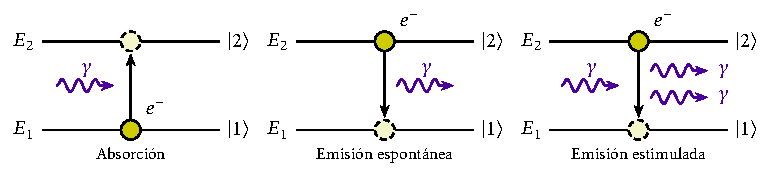
\includegraphics[width=\textwidth]{Figuras/ch1_rad_mat.pdf}
  \caption{A la derecha, absorción de un fotón con energía $E_{2} - E_{1} = \hslash \omega$, excitando el electrón y pasando del estado inferior $\ket{1}$ al superior $\ket{2}$. En el centro, emisión espontánea de un fotón con energía $E_{2}-E_{1}=\hslash \omega$, desexcitándose el electrón y pasando del estado $\ket{2}$ al estado $\ket{1}$. A la izquierda, emisión estimulada de un fotón con energía $E_{2}-E_{1}=\hslash \omega$ desde el estado excitado $\ket{2}$ hasta el estado inicial $\ket{1}$, debido a la estimulación del fotón incidente idéntico al emitido.}
  \label{fig:1.2}
\end{figure}

En la naturaleza, normalmente, los electrones ligados a un átomo (o los propios átomos, partículas cargadas, núcleos atómicos, moléculas, etc.) tienen sus niveles de energía ocupados siguiendo las leyes de la mecánica (del equilibrio) estadística. En esta situación de equilibrio termodinámico, la relación entre las poblaciones de estos niveles viene dada por la ley de Boltzmann \autocite{Feynman2011}
\begin{equation}\label{eq:1.0}
  \frac{N_{2}}{N_{1}} = \exp \left(-\frac{E_{2}-E_{1}}{k_{B}T}\right) < 1, 
\end{equation}
entre el número de electrones $N_{2}$ en el estado $\ket{2}$ y el número de electrones $N_{1}$ en el estado $\ket{1}$. En la ecuación \eqref{eq:1.0}, $T$ es la temperatura, por ejemplo, de un grupo de moléculas, $k_{B}$ es la constante de Boltzmann, y por simplicidad los estados se asumen no degenerados (un solo estado posible para cada nivel de energía), aunque esta simplificación desaparecerá más adelante. Como el número de electrones en el estado inferior $\ket{1}$ es mayor que en el estado superior $\ket{2}$, un haz de luz en camino sufrirá más absorción que emisión estimulada.

En cambio, en ocasiones puede presentarse la situación contraria en la naturaleza o en un laboratorio, encontrándose un grupo de átomos en una \emph{inversión de población} con $N_{2} > N_{1}$. Ambos estados tendrían una \enquote{temperatura negativa} respecto al otro. La luz que se propaga a través de medios con una inversión de población experimenta más emisión estimulada que absorción, amplificándose en el proceso. El resultado es la amplificación de luz por emisión estimulada de radiación, o efecto \enquote{láser}.

El aspecto clave del efecto láser es la inversión de población del medio activo. Sin embargo, la inversión de población es incompatible con el equilibrio termodinámico: por tanto, para conseguir la amplificación es necesario manipular la materia de alguna forma fuera del equilibrio. En la mayoría de los casos, esto se hace siguiendo alguna variante del proceso mostrado en los niveles de energía de la Figura \ref{fig:1.3}. 

Escogiendo un mecanismo de bombeo (para depositar energía) adecuado, los electrones son excitados rápidamente desde el nivel fundamental hasta una banda de estados de absorción característica del átomo o molécula en cuestión. Después, los electrones decaen rápidamente desde los estados de absorción hasta el estado $\ket{2}$, que es metaestable (su tiempo de permanencia en ese estado es mucho mayor que el tiempo de emisión espontánea), quedando los electrones \enquote{esperando} ahí. La transición responsable del efecto láser sucede del estado $\ket{2}$ al estado $\ket{1}$. 

\begin{figure}[htbp]
  \centering
  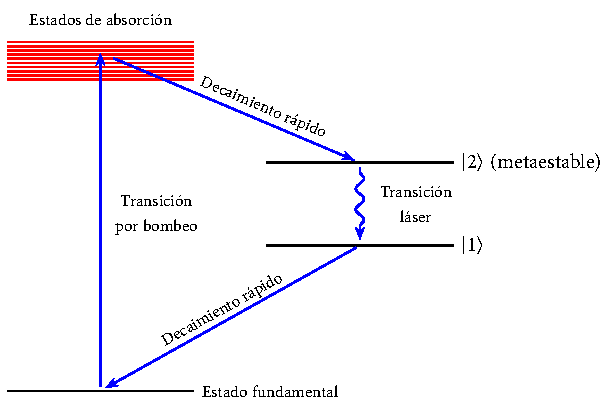
\includegraphics[width=0.7\textwidth]{Figuras/ch1_4_level_sch.pdf}
  \caption{Esquema de cuatro niveles para generar la inversión de población y conseguir el efecto láser. Las líneas horizontales representan los niveles de energía del sistema y las flechas representan las transiciones entre los distintos niveles. Adaptado de Thorne y Blandford (2017)\autocite{Thorne2017}.}
  \label{fig:1.3}
\end{figure}

Una vez los electrones decaen hasta el estado $\ket{1}$, vuelven a decaer rápidamente hasta el estado fundamental para después, posiblemente, volver a ser bombeados devuelta hasta los estados de absorción. Este mecanismo es conocido como \enquote{bombeo de cuatro niveles} (\emph{four-level pumping} en inglés), mientras que si el estado $\ket{1}$ es el estado fundamental se denomina \enquote{bombeo de tres niveles} (\emph{three-level pumping}). Además, también suele hacerse una distinción especial con un tercer esquema denominado \enquote{bombeo de cuasi-tres niveles} (\emph{quasi-three level pumping}) cuando el estado inferior de la transición láser $\ket{1}$ tiene una energía ligeramente superior al estado fundamental. La sección \S\ref{sec:3.3} mostrará como, de hecho, el esquema empleado por el experimento estudiado en este proyecto pertenece precisamente a este último caso.

La idea básica consiste en que, si el sistema de bombeo es capaz de actuar de forma rápida y súbita (con otro láser, por ejemplo), este proceso produce una inversión de población temporal entre los estados $\ket{2}$ y $\ket{1}$, gracias al cual una ráfaga incidente, relativamente débil de luz o \enquote{semilla} puede interaccionar con estos estados emitiendo una ráfaga de luz amplificada. El resultado es un láser pulsado, como el simulado durante el capítulo \S\ref{cap:4}. En el caso de tener un sistema de bombeo que funcione de forma continua, podría conseguirse como resultado una inversión poblacional permanente mediante el cual las \enquote{semillas} de luz incidentes puedan interaccionar, produciendo una luz láser de onda continua, en lugar de pulsada.

Mientras que el láser viaja a través del medio activo (los electrones fuera del equilibrio, en inversión de población), el flujo de energía $F$ aumenta con la distancia $z$ tal que $\symrm{d}F/\symrm{d}z = F/l_{o}$, entonces $F(z) = F_{o}\eu^{z/l_{o}}$. $F_{o}$ es el flujo inicial, y $l_{0} \equiv 1/|\mu|$ (longitud de amplificación en un factor $\symrm{r}$) depende de la intensidad de la inversión poblacional y de la intensidad del \enquote{acoplamiento} entre la luz y el medio activo. Normalmente, $l_{o}$ es demasiado grande como para conseguir un efecto láser suficientemente intenso en un solo recorrido de la luz por el medio activo. En estos casos, la amplificación hay que potenciarla introduciendo el medio activo en el interior de una \emph{cavidad de Fabry-Perot} (esquema en la Figura \ref{fig:1.4}), llamada frecuentemente \emph{cavidad resonante}.

\begin{figure}[htbp]
  \centering
  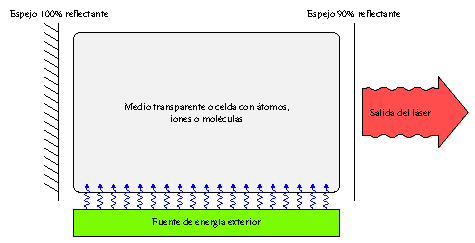
\includegraphics[width=0.7\textwidth]{Figuras/ch1_cavidad.pdf}
  \caption{Esquema de un cavidad de Fabry-Perot o cavidad resonante utilizada para mejorar la interacción de la luz láser con el medio activo. Adaptado de Milonni y Eberly (1988)\autocite{Milonni1988}.}
  \label{fig:1.4}
\end{figure}

La longitud $L$ de la cavidad se ajusta para optimizar la potencia obtenida, que se obtiene cuando la frecuencia $\omega = (E_{2}-E_{1})/\hslash $ es una frecuencia de resonancia (un modo) de la cavidad. Cuando esto sucede, la transición láser excita un modo de la cavidad asociado a una onda estacionaria, escapando la luz amplificada a través uno o ambos espejos de la cavidad. Si $\eta$ es el rendimiento de la cavidad (aproximadamente el número medio de veces que un fotón es reflejado hacia delante y hacia atrás dentro de la cavidad antes de escapar a través del espejo), entonces la cavidad incrementa la distancia que los fotones pueden recorrer a través del medio activo en un factor $\sim \eta$, incrementando entonces el flujo de energía saliente en un factor $\sim \eu^{\eta L/l_{o}}$.

Realmente, hay múltiples modos de Fabry-Perot excitados por una transición láser, de forma que la amplificación contiene varios modos y es una mezcla de diferentes polarizaciones. Para conseguir un solo modo y polarización, hay que incorporar elementos ópticos en la salida del láser para transmitir únicamente la polarización pura deseada, y después todos los modos excepto uno pueden eliminarse de la luz saliente mediante varias técnicas (utilizando una segunda cavidad de Fabry-Perot, por ejemplo).

Con un láser ideal (con una fuente de bombeo continua capaz de mantener una inversión de población perfecta, consiguiendo un emisión láser también perfecta), la luz conseguida tiene el estado más perfecto que la mecánica cuántica permite. Estos estados, llamados \emph{estados cuánticos coherentes}, tienen un campo eléctrico puro que oscila sinusoidalmente, superpuesto con la menor cantidad de ruido (desviaciones en la fase y la amplitud) que admite la teoría cuántica: las fluctuaciones cuánticas del vacío. El valor de las oscilaciones de la fase $\varphi$ están determinadas por el valor de la fase de la semilla responsable de activar la transición láser. Los láseres reales tienen un ruido adicional debido a una multitud de factores, aunque en cualquier caso, la luz conseguida suele ser altamente coherente, con tiempos de coherencia elevados, como aparecerá mostrado en la sección \S\ref{sec:1.1.2}.

\paragraph{Tipos de láseres y aplicaciones}
Como ha podido verse en esta sección \S\ref{sec:1.1.1}, los láseres pueden tener una emisión continua, altamente monocromática, o pueden ser pulsados. El medio activo puede ser un líquido, un gas (ionizado o neutro), o un sólido (semiconductores, vidrios, o cristales, típicamente dopados con impurezas). Los láseres pueden emplear como sistema de bombeo radiación electromagnética (una lámpara de luz suficientemente intensa, por ejemplo), colisiones atómicas que exciten los átomos responsables de las transiciones láser, reacciones químicas fuera del equilibrio, o campos eléctricos producidos por descargas eléctricas (los diodos láser de semiconductores bombeados por baterías comunes utilizados en comunicaciones ópticas).

Los pulsos láser pueden conseguirse activando y desactivando la fuente de bombeo, empleando la técnica conocida como \emph{mode-locking} (esencialmente consiste en inducir una interferencia destructiva entre ciertos modos de la cavidad de Fabry-Perot), o utilizando el esquema llamado \emph{Q-switching} (interrumpiendo el efecto láser, por ejemplo, introduciendo en la cavidad un material electro-óptico capaz de absorber la luz hasta que la fuente de bombeo haya producido una inversión de población suficientemente grande, para después aplicar un campo eléctrico sobre el material absorbente que lo hace transparente y recupera la operación láser.)

Un pulso láser puede llegar a tener duraciones de pocos femtosegundos (permitiendo realizar investigación básica en química de reacciones ultrarrápidas \autocite{Zewail2000}) incluso centenares de attosegundos ---ver sección \S\ref{sec:1.1.2}--- y pueden llegar a transportar energía de \qty{20000}{J} con duraciones de decenas de picosegundos y potencias de $\sim \qty{e15}{W}$ (por ejemplo, en la \emph{\acrfull{nif}} en Livermore, California, para la fusión por confinamiento inercial \autocite{Hurricane2019,Zylstra2022}).

El láser más potente de los Estados Unidos, en operación continua, es el \emph{\acrfull{miracl}}, desarrollado por la Armada para derribar misiles intercontinentales y satélites, con una potencia de $\sim \qty{1}{MW}$ en un rayo de $14 \times 14 $ \unit{cm^{2}} y $\sim \qty{70}{s}$ de duración \autocite{Thorne2017}. Los láseres de \ce{CO2} en continuo, con potencias de $\sim \qty{3}{kW}$, son comunes en la industria para cortar y soldar metales.

Un haz de alta potencia $\sim \qty{1}{GW}$ en un láser de \ce{CO2} operando con la técnica \emph{Q-switching} puede focalizarse en una región cuya sección transversal tiene unas dimensiones tan pequeñas como una longitud de onda de $\sim \qty{1}{µm}$, proporcionando intensidades de $\sim \qty{e21}{W/cm^{2}}$, inducciones magnéticas con valores cuadráticos medios de $\sim \qty{3}{kT}$, campos eléctricos de $\sim \qty{1}{TV/m}$ y diferencias de potencial en una sola longitud de onda de $\sim \qty{1}{MeV}$. Estos órdenes de magnitud son tan enormes que algunos de estos láseres de alta potencia pueden crear plasmas formados por pares electrón-positrón.

También existen muchas aplicaciones en ciencia e industria donde no se necesitan altas potencias, pero sí frecuencias de emisión elevadas con buena estabilidad, es decir, largos tiempos de coherencia. En estas situaciones, es habitual utilizar el esquema \emph{mode-locking} para fijar la frecuencia emitida en el rango óptico de una transición atómica (por ejemplo, los relojes atómicos de \ce{Al+}), consiguiendo estabilidades en frecuencia de $\Delta f/f \sim 10^{-17}$, obteniendo anchos de banda de $\Delta f \sim \qty{3}{mHz}$ durante horas o incluso más, con tiempos de coherencia de $\sim \qty{100}{s}$ y longitudes de coherencia de $\sim \qty{3e7}{km}$. 

Alternativamente, escogiendo la frecuencia de un modo muy estable en el interior de la cavidad de Fabry-Perot, se han conseguido alcanzar estabilidades de $\Delta f/f \sim 10^{-16}$ durante intervalos de $\sim \qty{1}{h}$ (cavidades que utilizan materiales superconductores como el Niobio), y $\Delta f/f \sim 10^{-22}$ durante unos pocos milisegundos \autocite{Mueller2016,Kwee2012} en los brazos de \qty{4}{km} del interferómetro para la detección de ondas gravitacionales (la colaboración \emph{\acrfull{ligo}} que anunció el descubrimiento de las ondas gravitacionales en $2016$ \autocite{Abbott2016}).

Nuevamente, queda demostrado que desde su creación en $1960$ por Maiman, los láseres permean todos los aspectos de la vida cotidiana y las tecnologías más avanzadas del mundo. Desde los lectores de códigos de barras en los supermercados, hasta los punteros láser, reproductores DVD, cirugía oftalmológica, impresoras láser, cortadoras y soldaduras láser, giroscopios láser (que son bastante utilizados en los aviones comerciales), espectroscopía de Raman, fusión por confinamiento inercial, comunicaciones ópticas, ordenadores basados en circuitos ópticos, holografía y relojes atómicos, constituyen solo algunos ejemplos presentes en la actualidad que, sin ser en absoluto conscientes en la mayoría de ocasiones, facilitan y mejoran la vida de la sociedad en su conjunto.

Para detallar y completar el proceso de interacción radiación-materia, desde una perspectiva más general (como se prometió al principio de esta sección \S\ref{sec:1.1.1}), y prestando atención a las condiciones necesarias para conseguir la amplificación, el siguiente apartado presenta un análisis más exhaustivo. 

\paragraph{Condiciones para la amplificación}
La aproximación más sencilla \autocite{Schwartz2013} para cuantificar los procesos de interacción entre la luz y la materia emplea los conocidos \emph{coeficientes de Einstein}. Estos coeficientes proporcionan las tasas de emisión y absorción de luz por parte de un átomo (o iones, moléculas, etc.) excitado. Estos fenómenos ya habían sido observados a principios del siglo $\symrm{XX}$ en reacciones químicas y en la radiactividad natural, pero la relación entre la emisión y absorción apareció de la mano de Einstein (como se adelantó en la sección \S\ref{sec:1.1.1}) en dos artículos \autocite{Einstein1916,Einstein1916a} publicados en $1916$ utilizando la incipiente teoría cuántica.

El razonamiento de Einstein seguía esta idea: en una cavidad (por ejemplo, de Fabry-Perot para un láser) en cuyo interior hay átomos con energías $E_{1}$ y $E_{2}$, y un número de átomos $N_{1}$ y $N_{2}$, respectivamente, tal que 
\begin{equation}\label{eq:1.1}
  \nu = \frac{E_{2}-E_{1}}{h},
\end{equation}
la probabilidad de emitir espontáneamente un fotón de frecuencia $\nu$ cuando un átomo evoluciona del estado de mayor a menor energía es conocida como \emph{coeficiente de emisión de espontánea} $A_{21}$. Por otro lado, la probabilidad de un fotón de inducir la transición $2 \rightarrow 1$ es proporcional al \emph{coeficiente de emisión estimulada} $B_{21}$ y a la densidad de energía espectral $\rho(\nu)$ (proporcional al número de fotones) de los fotones de frecuencia $\nu$ dentro de la cavidad. Estos coeficientes contribuyen al cambio de la población del nivel superior tal que 
\begin{equation}\label{eq:1.2}
  \diff N_{2} = -\left[A_{21} + B_{21} \rho(\nu)\right]N_{2} + \cdots.
\end{equation}
En cambio, la probabilidad de un fotón de inducir la transición $1 \rightarrow 2$ se denomina \emph{coeficiente de absorción} $B_{12}$, disminuyendo la población del nivel inferior e incrementando la del superior debido a la absorción en un factor $B_{12} \rho(\nu)N_{1}$. Como el número total de átomos es constante en este sistema, $\diff N_{2}+\diff N_{1}=0$, por tanto,
\begin{equation}\label{eq:1.3}
  \diff N_{2} = -\diff N_{1} = -\left[A_{21} + B_{21} \rho(\nu)\right]N_{2} + B_{12} \rho(\nu)N_{1}.
\end{equation}
La densidad $\rho_{\nu}$ podría corresponderse con la energía de un haz láser penetrando a través del medio activo en el interior de una cavidad. En este punto, Einstein asume una situación de equilibrio de los átomos bajo la hipótesis del cuerpo negro. En equilibrio, las poblaciones son constantes, $\diff N_{1} = \diff N_{2} = 0$, y pueden calcularse a partir de la distribución de Maxwell-Boltzmann \autocite{Feynman2011} 
\begin{align}
  \label{eq:1.4a}
  N_{1} &= N \eu^{-\beta E_{1}}, \\
  \label{eq:1.4b}
  N_{2} &= N \eu^{-\beta E_{2}}.
\end{align}
En las ecuaciones \eqref{eq:1.4a} y \eqref{eq:1.4b}, el factor $\beta = 1/(k_{B}T)$, mientras que $N$ es un factor para normalizar la función de probabilidad asociada a ambos estados a la unidad. Para obtener una relación del equilibrio entre poblaciones, basta combinar la condición de equilibrio entre los dos niveles junto a la estadística de Maxwell-Boltzmann, obteniendo 
\begin{equation}\label{eq:1.5}
  \left[B_{12}\eu^{-\beta E_{1}}-B_{21}\eu^{-\beta E_{2}}\right] \rho(\nu) = A_{21}\eu^{-\beta E_{2}},
\end{equation}
y despejando la densidad de energía, empleando la ecuación \eqref{eq:1.1}
\begin{equation}\label{eq:1.6}
  \rho(\nu) = \frac{A_{21}}{B_{12}\eu^{h \nu/(k_{B}T)} - B_{21}}.
\end{equation}
Sin embargo, el cuerpo negro en equilibrio tiene una densidad espectral de energía \autocite{Feynman2011}
\begin{equation}\label{eq:1.7}
  \rho(\nu) = \frac{8 \pi h \nu^{3}}{c^{3}}\frac{1}{\eu^{h \nu/(k_{B}T)} - 1},
\end{equation}
y la condición de equilibrio debe cumplirse para cualquier temperatura en el interior de la cavidad, por lo que comparando las ecuaciones \eqref{eq:1.6} y \eqref{eq:1.7} los coeficientes deben cumplir
\begin{align}
  \label{eq:1.8a}
  B_{12} &= B_{21}, \\
  \label{eq:1.8b}
  \frac{A_{21}}{B_{21}} &= \frac{8 \pi h \nu^{3}}{c^{3}}.
\end{align}
Las implicaciones de estos resultados son considerablemente importantes. En primer lugar, la ecuación \eqref{eq:1.8a} dice que los coeficientes de absorción y emisión estimulada son iguales. Estos coeficientes pueden calcularse en mecánica cuántica \autocite{Sakurai2020} con relativa facilidad utilizando métodos perturbativos en presencia de un campo electromagnético externo, luego el coeficiente de emisión espontánea $A_{21}$ quedaría determinado. En segundo lugar, la ecuación \eqref{eq:1.8b} implica que para grandes frecuencias, la emisión espontánea domina frente a la emisión estimulada, haciendo más difícil conseguir un láser para frecuencias muy elevadas. 

Además, este último hecho motiva la extrema dificultad de la amplificación de láseres de rayos X blandos, como mostrará la sección \S\ref{sec:1.4}, necesitando emplear métodos de bombeo que depositen grandes cantidades de energía, suficientes para conseguir una inversión de población que \enquote{compense} las altas frecuencias de la radiación \acrshort{xuv}. 

Ahora bien, la situación general tiene que considerar la posibilidad de que los estados involucrados en la transición sean degenerados, por lo que hay introducir la multiplicidad de estados posibles con la misma energía, de forma que ahora la ecuación \eqref{eq:1.0} es
\begin{equation}\label{eq:1.9}
  \frac{N_{2}}{N_{1}} = \frac{g_{2}}{g_{1}}\exp \left(-\frac{E_{2}-E_{1}}{k_{B}T}\right), 
\end{equation}
con $N_{2}$ y $N_{1}$ las poblaciones de los niveles con energías $E_{2}$ y $E_{1}$, respectivamente, donde $g_{2}$ y $g_{1}$ son el número de estados (pueden entenderse como subniveles de igual energía) posibles con dichas energías. En este caso, la inversión de población necesita que \autocite{Tallents2003}
\begin{equation}\label{eq:1.10}
  \tcboxmath{\frac{N_{2}}{g_{2}} > \frac{N_{1}}{g_{1}},}
\end{equation}
pues la función exponencial está acotada superiormente por $1$ para temperaturas positivas del medio activo. 

La consideración de estados degenerados tiene la ventaja de eliminar la noción de temperatura \enquote{negativa} que aparecía de forma natural cuando cada energía tenía un solo estado asociado posible (aunque una temperatura negativa no tiene sentido físicamente, porque la distribución de Boltzmann solo es válida para un medio en equilibrio termodinámico), pero ahora la degeneración de los estados involucrados es la relación que determina la posibilidad de conseguir la inversión.

Rápidamente, a partir de la ecuación \eqref{eq:1.9} se deduce que si las poblaciones están en equilibrio, es imposible tener una inversión de población entre ambos estados. Las relaciones entre los coeficientes de Einstein quedan como 
\begin{empheq}[box=\tcbhighmath]{align}
  \label{eq:1.11a}
  g_{1}B_{12} &= g_{2}B_{21}, \\
  \label{eq:1.11b}
  \frac{A_{21}}{B_{21}} &= \frac{8 \pi h \nu^{3}}{c^{3}},
\end{empheq}
luego los coeficientes de absorción y emisión estimulada de radiación no son, en general, iguales cuando los estados que participan en la transición láser son degenerados, recuperándose la ecuación \eqref{eq:1.8a} cuando cada nivel de energía pertenece a un único estado.

\paragraph{Coeficiente de ganancia}
El coeficiente de absorción $\mu$ de cualquier sustancia tiene un carácter fuertemente dependiente de la frecuencia de la luz que interacciona con el medio absorbente, es decir, existen regiones del espectro de frecuencias donde la absorción puede ser muy intensa, o no producirse en absoluto. Exactamente la misma dependencia ocurre durante el proceso de emisión estimulada, como mostraba la dependencia de la frecuencia de la densidad espectral de energía $\rho(\nu)$ en el interior de la cavidad. Para estudiar el proceso de amplificación de la luz láser, conviene definir un \emph{coeficiente de ganancia} $G(\nu) = +|\mu(\nu)|$ (simplemente consiste en el coeficiente de atenuación $\mu$ cambiado de signo) para reflejar esta naturaleza espectral.

La emisión espontánea es un proceso puramente estocástico (aleatorio) en la dirección, fase, polarización y frecuencia de los fotones emitidos. La aleatoriedad de las frecuencias emitidas sigue una distribución (normalizada a la unidad bajo integración) o \emph{función de línea} $f(\nu)$, cuya expresión depende de los procesos de interacción dominantes ocurridos en el medio activo. Cuando los choques entre las partículas constituyentes del medio activo son el fenómeno más importante (llamado \emph{ensanchamiento colisional}) que determina la amplitud del perfil de frecuencias, la emisión describe una función \enquote{de Lorentz} dada por \autocite{Milonni1988,Tallents2003,Svelto2010}
\begin{equation}\label{eq:1.12}
  f_{L}(\nu) = \frac{2}{\pi \Delta \nu_{L}}\frac{1}{1 + \left(4 \nu^{2}/(\Delta \nu_{L})^{2}\right)},
\end{equation}
donde $\Delta \nu_{L}$ es la diferencia de frecuencias (ancho de banda) tal que el valor de la distribución es exactamente la mitad de su valor máximo en los extremos de dichas frecuencias, el máximo ancho de banda para la mitad del pico máximo producido, habitualmente conocido como \emph{\acrfull{fwhm}}, representado en la Figura \ref{fig:1.5}. 

\begin{figure}[htbp]
  \centering
  \begin{subcaptionblock}{.4\textwidth}
    \centering
    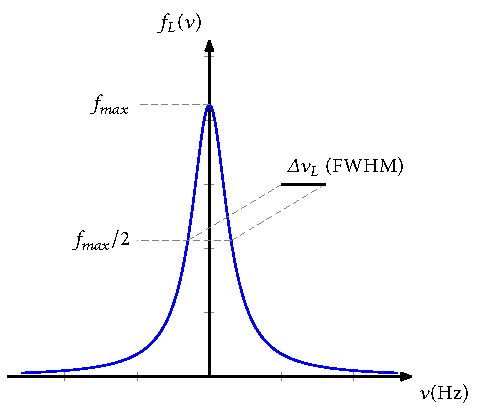
\includegraphics[width=\textwidth]{Figuras/ch1_lorentz.pdf}
    \caption{Perfil Lorentziano}\label{fig:ch1_linefuna}
  \end{subcaptionblock}
  \begin{subcaptionblock}{.4\textwidth}
    \centering
    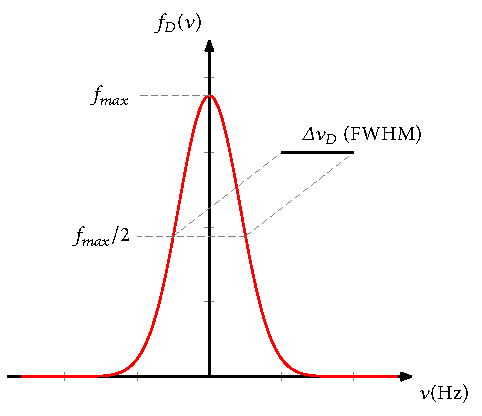
\includegraphics[width=\textwidth]{Figuras/ch1_doppler.pdf}
    \caption{Perfil Doppler}\label{fig:ch1_linefunb}
  \end{subcaptionblock}
  \caption{Perfiles de línea gaussiano y exponencial junto al \acrshort{fwhm}. \textbf{a}, Función de línea de Lorentz para los efectos térmicos dominantes. \textbf{b}, Función de línea de Doppler para los efectos de las colisiones dominantes.}
  \label{fig:1.5}
\end{figure}

Por otro lado, en un plasma, cuando la energía térmica del movimiento oscilatorio de las partículas, es decir, la temperatura, es dominante (como sucede con los iones del plasma empleado en este proyecto, ver sección \S\ref{1.4}), la función de línea $f_{D}(\nu)$ sigue una distribución Gaussiana, debida al efecto Doppler de la luz emitida por los iones en su movimiento térmico (llamado \emph{ensanchamiento Doppler})  cuando la velocidad de los iones está descrita por una distribución de Maxwell, pudiendo escribir \autocite{Tallents2003,Milonni1988,Oliva2010}
\begin{equation}\label{eq:1.13}
f_{D}(\nu) = \frac{2}{\Delta \nu_{D}} \left(\frac{\ln 2}{\pi}\right)^{1/2} \exp \left(-4 \ln(2) \frac{\nu^{2}}{(\Delta \nu_{D})^{2}}\right),
\end{equation}
con $\Delta \nu_{D}$ el \acrshort{fwhm} del perfil de línea $f_{D}(\nu)$. En este caso, $\Delta \nu_{D}$ depende de la temperatura $T_{i}$ de los iones involucrados en la transición láser según la ecuación
\begin{equation}\label{eq:1.14}
  \Delta \nu_{D} = 2(\ln 2)^{1/2} \frac{1}{\lambda}\left(\frac{m_{i}}{2k_{B}T_{i}}\right)^{1/2},
\end{equation}
siendo $m_{i}$ la masa de los iones y $\lambda$ la longitud de onda de la emisión láser. En el centro del perfil, la función puede aproximarse como
\begin{equation}\label{eq:1.15}
  f_{D}(0) = \lambda \left(\frac{m_{i}}{2 \pi k_{B}T_{i}}\right)^{1/2}.
\end{equation}
La amplificación de la intensidad láser $I(\nu)$ para una frecuencia $\nu$ debida a la emisión estimulada de luz puede calcularse mediante un balance de transferencia radiativa \autocite{Milonni1988}
\begin{equation}\label{eq:1.16}
  \pdv{I(z,\nu)}{z} = G(\nu)I(z,\nu) + E(\nu),
\end{equation}
con $z$ la distancia recorrida en el medio amplificador, $E(\nu)$ la tasa de emisión espontánea para un ángulo sólido determinado y $G(\nu)$ el coeficiente de ganancia. En la ecuación \eqref{eq:1.16}, puede observarse que la intensidad $I(z,\nu)$ tendrá aproximadamente como solución una función exponencial creciente en la dirección $z$, siempre y cuando el coeficiente de ganancia no sea demasiado pequeño en comparación con la tasa de emisión espontánea $E(\nu)$. En tal circunstancia, el comportamiento de la intensidad, como aparece esquemáticamente en la Figura \ref{fig:1.6}, es
\begin{equation}\label{eq:1.17}
  I(z,\nu) = I_{0}\eu^{G(\nu)z},
\end{equation}
donde $I_{0}$ es la intensidad inicial de la luz láser antes de comenzar la amplificación. Si $G(\nu)$ fuera negativo, esto es, sustituyéndolo por el coeficiente de absorción $\mu(\nu)$, la ecuación recuperaría el proceso de absorción de luz característico de un medio absorbente, como cabría esperar. 

\begin{figure}[htbp]
  \centering
  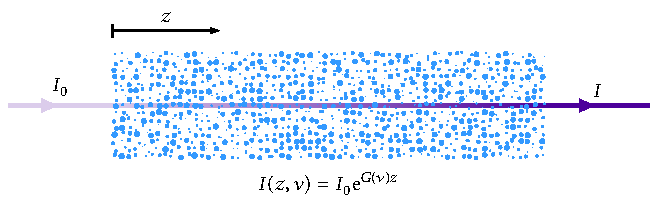
\includegraphics[width=0.8\textwidth]{Figuras/ch1_lambeer.pdf}
  \caption{Solución del balance radiativo cuando la tasa de emisión espontánea $E(\nu)$ es despreciable. La intensidad del haz láser $I(z,\nu)$ aumenta exponencialmente con la distancia de propagación $z$.}
  \label{fig:1.6}
\end{figure}

En un sistema de dos estados, como el representado en la Figura \ref{fig:1.3}, la tasa de emisión espontánea en una región de frecuencias próxima a la de transición es \autocite{Tallents2003}
\begin{equation}\label{eq:1.18}
  E(\nu) = N_{2}A_{21}f(\nu)h \nu\frac{\Omega}{4 \pi},
\end{equation}
con $\Omega$ el ángulo sólido escogido. Por otro lado, el coeficiente de ganancia viene dado por
\begin{equation}\label{eq:1.19}
  G(\nu) = \sigma(\nu)\left(N_{2}-\frac{g_{2}}{g_{1}}N_{1}\right),
\end{equation}
donde $\sigma(\nu)$ es la sección eficaz microscópica de la emisión estimulada. Cuando los dos estados partícipes $\ket{1}$ y $\ket{2}$ de la transición láser están en equilibrio térmico, puede demostrarse que la sección eficaz $\sigma(\nu)$ está relacionada con el coeficiente de Einstein para la emisión espontánea $A_{21}$ como \autocite{Tallents2003}
\begin{equation}\label{eq:1.20}
  \sigma(\nu) = f(\nu)\frac{\lambda^{2}}{8 \pi}A_{21},
\end{equation}
resultando entonces el coeficiente de ganancia cumplir la ecuación
\begin{equation}\label{eq:1.21}
  G(\nu) = f(\nu)\frac{\lambda^{2}}{8 \pi}A_{21}\left(N_{2}-\frac{g_{2}}{g_{1}}N_{1}\right).
\end{equation}
Como las poblaciones de los niveles de la transición son, en principio, desconocidas, una manera más sencilla de calcular la ganancia consiste en introducir una hipótesis de ensanchamiento del perfil de línea homogéneo \autocite{Tallents2003} en una situación de equilibrio entre ambos niveles poblacionales, tal que
\begin{equation}\label{eq:1.22}
  G(\nu) = \frac{g_{0}}{1+I_{av}/I_{s}}\frac{f(\nu)}{f(0)},
\end{equation}
siendo $I_{av}$ la intensidad láser promediada con la función de línea, $g_{0}$ el \enquote{pequeño} coeficiente de ganancia para el centro del perfil y $I_{s}$ la intensidad de saturación del láser. 

Estos elementos aparecen debido a la pérdida de población del estado superior $\ket{2}$ cuando la emisión estimulada es demasiado intensa, de forma que, a pesar del bombeo de energía, la inversión de población disminuye, perdiendo capacidad de amplificación en el proceso. Bajo esta casuística, cuando la intensidad alcanza saturación, el coeficiente de ganancia $G(\nu)$ disminuye hasta alcanzar la mitad del valor dado por $g_{0}$. Si la intensidad siguiera aumentando por encima de la saturación $I_{s}$, el coeficiente de ganancia disminuiría incluso más, comprometiendo la eficiencia del proceso. 

Regresando con la hipótesis anterior, y representando por $R$ la tasa de bombeo (relación entre la potencia de bombeo y la potencia de saturación por unidad de volumen del medio activo) desde el nivel fundamental hasta los niveles de absorción y $\tau_{0}$ el tiempo de vida medio del estado superior $\ket{2}$ (el tiempo medio que tarda un átomo en emitir espontáneamente un fotón y pasar al estado inferior $\ket{1}$), la intensidad de saturación $I_{s}$ y el pequeño coeficiente de ganancia $g_{0}$ son
\begin{align}
  \label{1.23a}
  g_{0} &\simeq f(0)\frac{\lambda^{2}}{8 \pi}A_{21} \tau_{0}R, \\
  \label{1.23b}
  I_{s} &\simeq \frac{8 \pi}{\lambda^{2}}\frac{h \nu}{f(0)A_{21} \tau_{0}}.
\end{align}

\begin{footheorem*}{Ganancia y condiciones de amplificación}
    Para conseguir producir una amplificación de la radiación efectiva, es necesario conseguir una inversión poblacional suficientemente grande que verifique
    \begin{equation}
      \tag{GC.1}
      \frac{N_{2}}{g_{2}} > \frac{N_{1}}{g_{1}},
    \end{equation}
    obteniéndose una intensidad $I(z,\nu)$ de la luz emitida aproximadamente descrita por la función
    \begin{equation}
      \tag{GC.2}
      I(z,\nu) = I_{0}\eu^{G(\nu)z},
    \end{equation}
    con $G(\nu)$ el coeficiente de ganancia para frecuencias próximas al efecto láser.
\end{footheorem*}

\subsection{Propiedades ópticas}\label{sec:1.1.2}
La radiación emitida por un láser está caracterizada principalmente por una alta monocromaticidad, coherencia, direccionalidad e intensidad. A estas propiedades puede añadirse una quinta relacionada con la duración de la emisión\autocite{Svelto2010}. Esta última hace referencia a la capacidad de generar pulsos de muy corta duración, propiedad que, aunque menos fundamental, tiene gran importancia en muchas aplicaciones. 

\paragraph{Monocromaticidad}
De forma simplificada, esta propiedad se debe fundamentalmente a dos motivos: en primer lugar, solamente una onda electromagnética de frecuencia $\nu=\omega/2 \pi$ dada por \eqref{eq:1.1} puede ser amplificada y, en segundo lugar, como los esquemas de espejos utilizados forman una cavidad resonante, las oscilaciones pueden producirse únicamente a las frecuencias de resonancia de esta cavidad. Esta última circunstancia implica que el ancho de banda $\Delta\nu$ de la emisión láser es habitualmente mucho menor ---hasta diez órdenes de magnitud--- que el ancho de banda observado en la transición $2\rightarrow 1$ durante la emisión espontánea asociada.

Por ejemplo, las últimas propuestas de láseres de Fabry-Perot para la fabricación de circuitos integrados ---Tran \emph{et al} (2022)\autocite{Tran2022}---, emplean frecuencias de \qty{300}{THz} ($\lambda = \qty{980}{nm}$) con anchos de banda $\Delta\nu = \qty{10}{kHz}$, resultando una anchura relativa para la frecuencia de emisión $\Delta\nu/\nu = 3,33\times 10^{-11}$. El espectro de la emisión láser tiene una alta pureza, como ilustra la Figura \ref{fig:1.7}, consiguiéndose reducir la dispersión a través de un medio de propagación dado y mejorando la focalización del haz, ya que el índice de refracción depende de la longitud de onda emitida.

\begin{figure}[htpb]
  \centering
  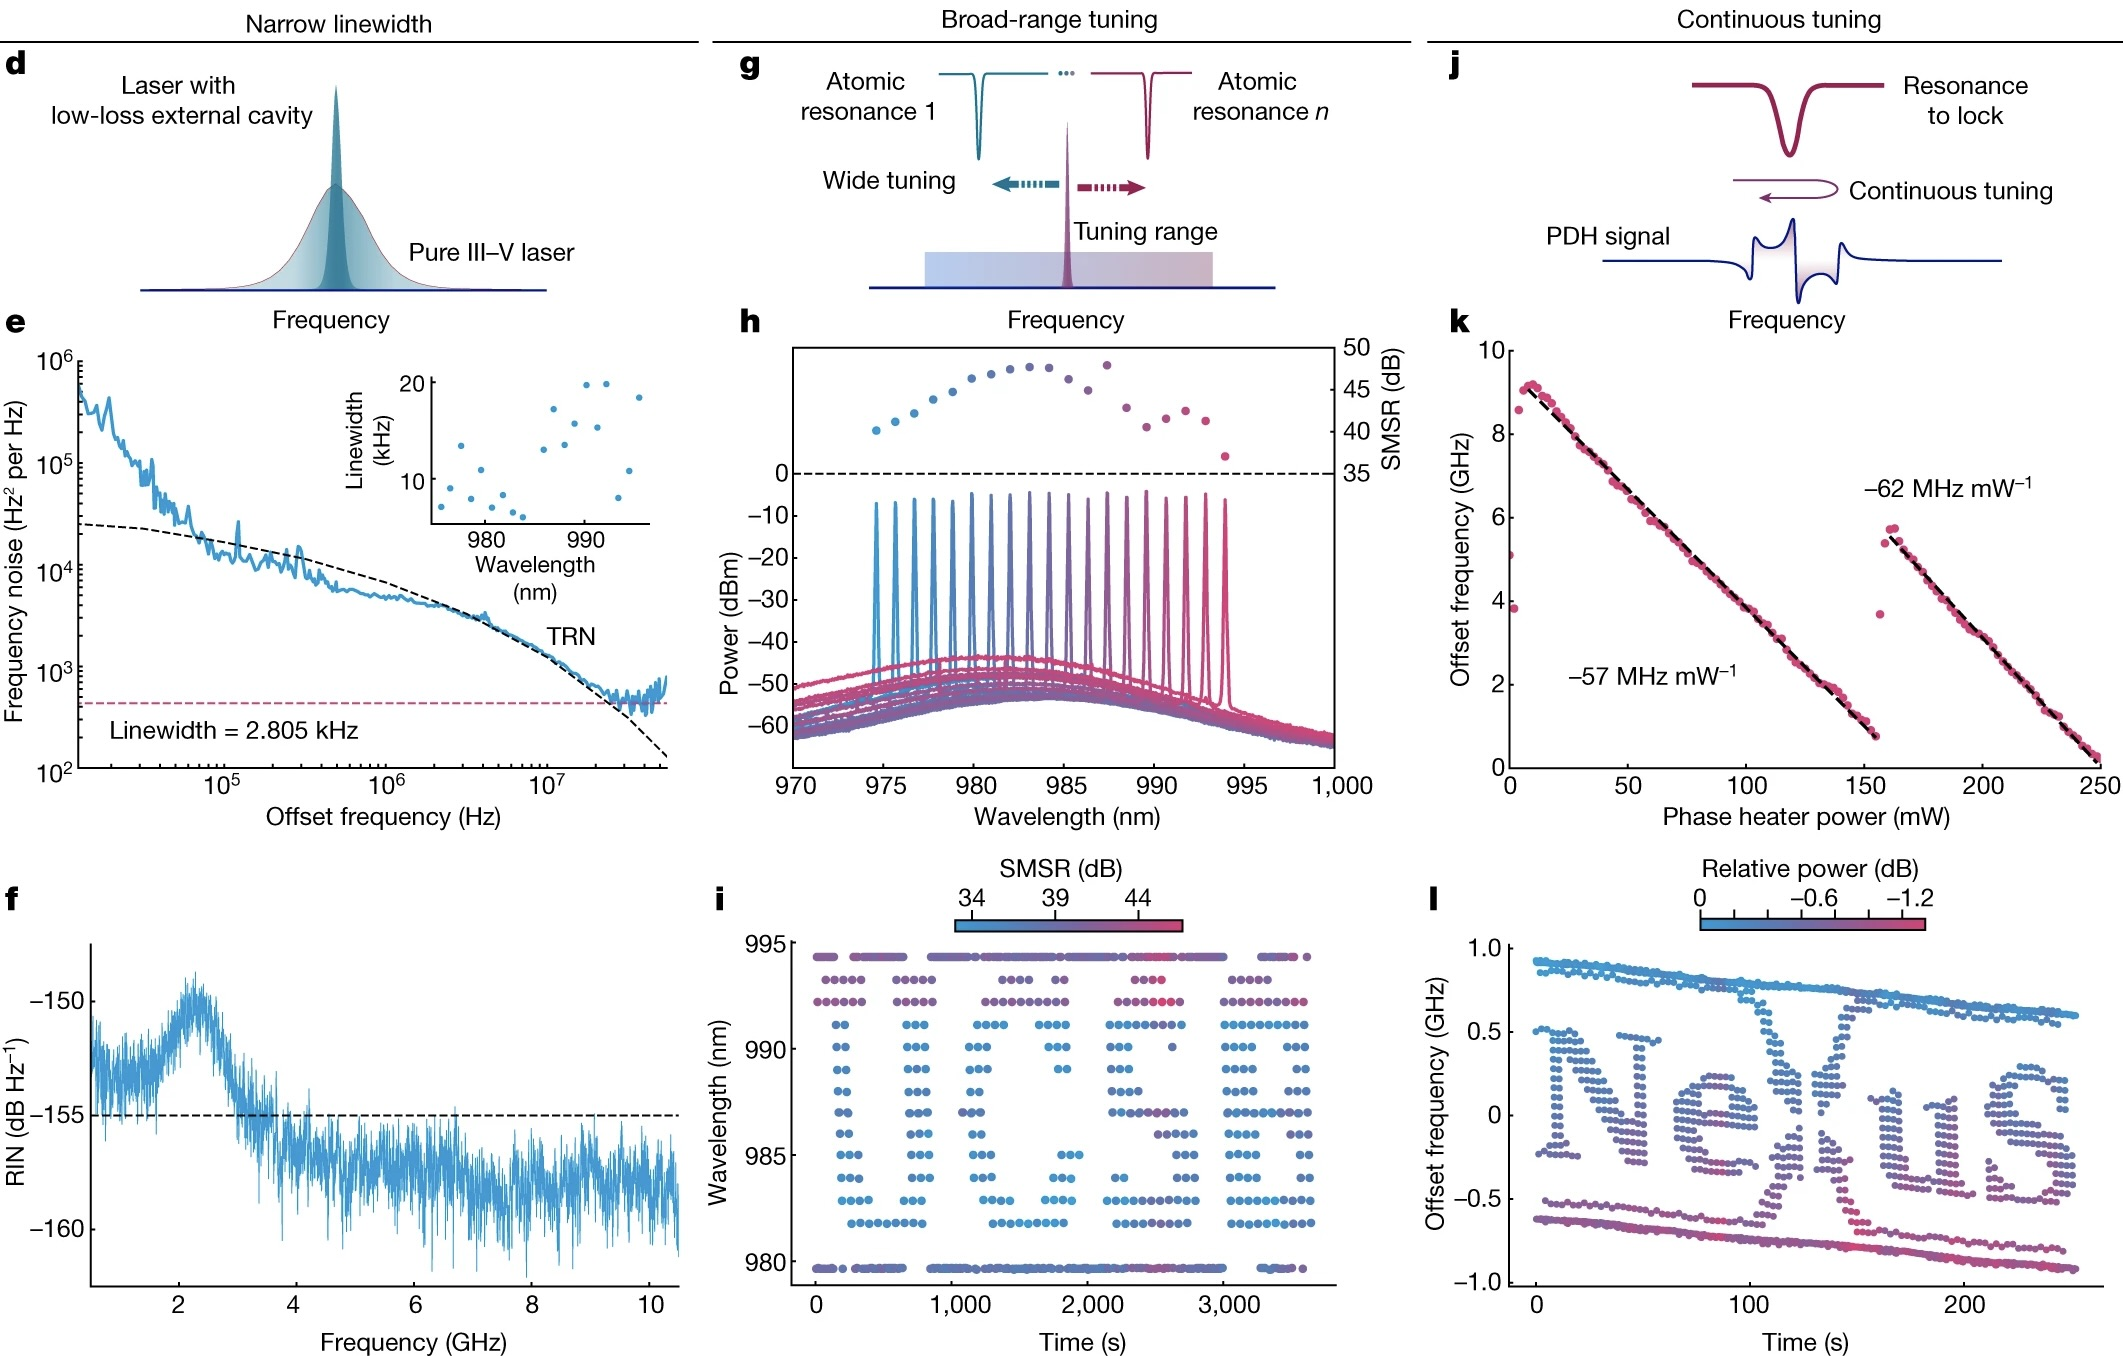
\includegraphics[width=\textwidth]{Figuras/ch1_amplif.png}
  \caption{Espectro de emisión del láser empleado en la propuesta de Tran \emph{et al} (2022)\autocite{Tran2022}. \textbf{d}, Ancho de banda conseguido con la cavidad resonante. \textbf{e}, Ruido en la frecuencia del espectro de emisión. \textbf{g}, Frecuencias de resonancia. \textbf{h}, Longitudes de onda de operación.}
  \label{fig:1.7}
\end{figure}

En realidad, la longitud de onda de la transición láser admite ---por el principio de incertidumbre de Heisenberg--- frecuencias de excitación distintas a la ecuación \eqref{eq:1.1}, tal que $\nu\rightarrow\nu + \delta\nu$. La magnitud de $\delta\nu$ es proporcional a la constante de Planck $h = \qty{6,626e-34}{J.s}$, siendo entonces extremadamente pequeña la variación introducida en el ancho de banda de la emisión láser debido a este fenómeno. 

Además, Schawlow y Townes demostraron que la anchura de banda mínima de un láser es la anchura de banda de la cavidad resonante dividida por dos veces el número de fotones $\langle n\rangle$ en el interior de la cavidad, límite conocido como \emph{\acrfull{sql}}. Sin embargo, existen grupos de investigación\autocite{Liu2021} que sugieren la posibilidad de utilizar circuitos superconductores para superar el \acrshort{sql} por un factor $\sim \xval{n}$ e incluso $\sim \xval{n}^{2}$, aproximándose al denominado \emph{límite de Heisenberg}.

\paragraph{Coherencia}
A primer orden, el concepto de coherencia de una onda electromagnética introduce dos conceptos, llamados coherencia espacial y temporal\autocite{Svelto2010}.

Para definir la coherencia espacial, basta con imaginar dos puntos $P_1$ y $P_2$ situados en el mismo frente de onda, en un instante inicial, de una onda electromagnética determinada, siendo $E_1(t)$ y $E_2(t)$ las amplitudes del campo eléctrico en dichos puntos. Por definición, el desfase entre ambos campos en ese instante es cero. Ahora bien, si en cualquier instante posterior, el desfase entre ambos mantiene un valor nulo, entonces se dice que ambos puntos tienen una coherencia perfecta. Si esto ocurre para cualquier par de puntos del frente de onda, entonces se dice que la onda tiene \emph{coherencia espacial perfecta}. En la práctica, para un punto $P_1$, el punto $P_2$ tiene que estar en un área muy próxima a $P_1$ para mantener una buena correlación entre ambas fases. En estos casos, existe una \emph{coherencia espacial parcial} y, para cualquier punto $P$, puede definirse un área de coherencia $S_{c}(P)$ apropiada.

Para definir la coherencia temporal, se supone el campo eléctrico de la onda anterior en un punto $P$, pero en dos instantes de tiempo $t$ y $t+\tau$. Si para un determinado intervalo $\tau$, el desfase entre las dos ondas se mantiene constante para cualquier instante de tiempo $t$, entonces se dice que tienen coherencia temporal durante el intervalo $\tau$. Si esto ocurre para cualquier $\tau$, la onda electromagnética tendrá una \emph{coherencia temporal perfecta}. En la práctica, el desfase puede mantenerse durante cualquier intervalo de tiempo $\tau$, tal que $0<\tau<\tau_0$, en cuyo caso la onda tiene \emph{coherencia temporal parcial} con un tiempo de coherencia $\tau_0$. En experimentos recientes ---Zhou \emph{et al} (2020)---\autocite{Zhou2020}, el láser de electrones libres (\acrshort{fel}) del \emph{\acrfull{lcls}} ha proporcionado pulsos de rayos X duros (\qty{60}{µJ}, \qty{3}{fs}) con un tiempo de coherencia parcial de $\tau_0 = \qty{174,7}{as}$ (\qty{1}{as} = \qty{e-18}{s}). La Figura \ref{fig:1.8} muestra los tiempos de coherencia obtenidos en dicho experimento (aunque puede parecer un tiempo de coherencia muy pequeño, hay que tener en cuenta que no puede superar la duración del pulso). 

Es importante mencionar que ambos conceptos de coherencia son independientes. De hecho, pueden darse casos de ondas con buena coherencia espacial y mala coherencia temporal, o viceversa. Además, como se ha comentado inicialmente, estas propiedades aparecen cuando se estudia el grado de coherencia de la onda a primer orden. Esta caracterización, en general, consiste en medir por ejemplo, mediante un interferómetro de Young, un elevado número de veces el campo eléctrico en dos puntos distintos del espacio $\symbf{r}_1$ y $\symbf{r}_2$ para dos instantes de tiempo $t_1$ y $t_2$ de un intervalo $T$, definiéndose el \emph{grado de coherencia de primer orden} como
\begin{equation}\label{eq:1.24}
  \gamma^{(1)}(\symbf{r}_{1},\symbf{r}_{2},t_{1},t_{2}) = \frac{\langle E(\symbf{r}_{1},t_{1})E^{*}(\symbf{r}_{2},t_{2}\rangle)}{\langle E(\symbf{r}_{1},t_{1})E^{*}(\symbf{r}_{1},t_{1}) \rangle^{1/2} \langle E(\symbf{r}_{2},t_{2})E^{*}(\symbf{r}_{2},t_{2}) \rangle^{1/2}},
\end{equation}
con $E^{*}$ el complejo conjugado del campo eléctrico. En esencia, la ecuación \eqref{eq:1.24} \enquote{ensambla} el valor medio de las mediciones realizadas para el campo eléctrico y las normaliza, permitiendo medir simultáneamente coherencia espacial y temporal de la onda.

\begin{figure}[htpb]
  \centering
  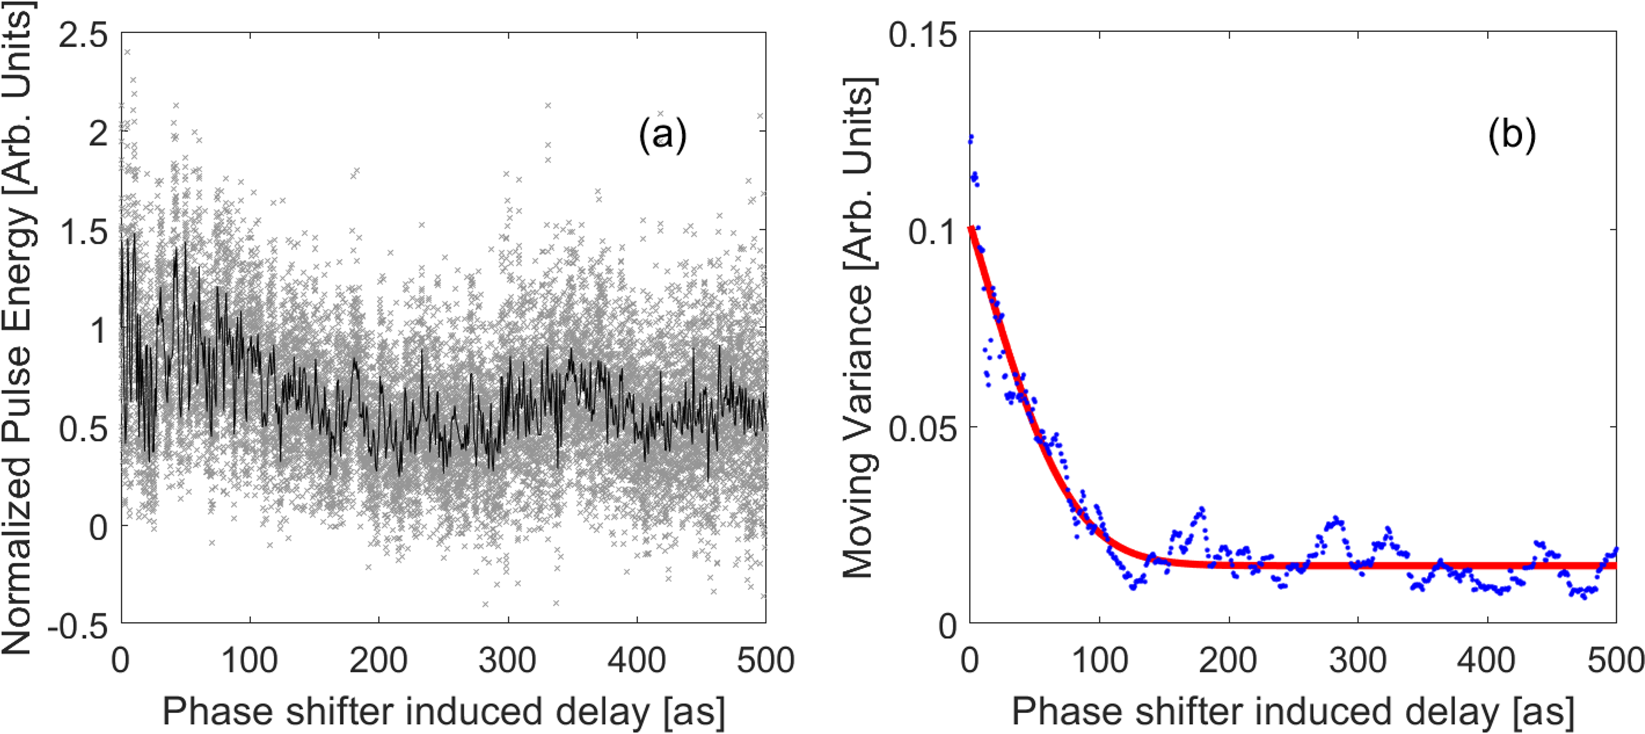
\includegraphics[width=0.8\textwidth]{Figuras/ch1_coher.png}
  \caption{Resultados experimentales del tiempo de coherencia medidos en el \acrshort{lcls}\autocite{Zhou2020}. \textbf{a}, Energía de los pulsos frente al retraso temporal. \textbf{b}, Cambios en la varianza respecto al retraso temporal.}
  \label{fig:1.8}
\end{figure}

El concepto de coherencia de primer orden hace referencia a que la medición realizada contempla la correlación entre amplitudes de ondas --el campo eléctrico---, mientras que la coherencia de orden $n$ expresa la correlación entre los productos de orden $n$ del campo eléctrico. Por ejemplo, a segundo orden ---el cuadrado del campo eléctrico---, la medición encierra la información sobre la intensidad del campo, de manera que la \emph{función correlación de orden} $n$ sería $\Gamma^{(n)}(\symbf{r}_1,t_1,\ldots,\symbf{r}_n,t_n) = \langle E(\symbf{r}_1,t_1)E^{*}(\symbf{r}_1,t_1)\ldots E(\symbf{r}_n,t_n)E^{*}(\symbf{r}_n,t_n)\rangle$.

\paragraph{Direccionalidad}
La emisión de un láser puede llegar a consistir en frentes de onda planos prácticamente ideales. La difracción es el único fenómeno ondulatorio que impone un umbral inferior en la divergencia del haz láser. El orden de magnitud del ángulo sólido $\Delta\Omega$ y el ángulo de divergencia $\Delta\theta$ dependen fundamentalmente de la longitud de onda $\lambda$ y el área de apertura $A$ de la emisión\autocite{Milonni1988} a través de la relación
\begin{equation}\label{eq:1.25}
    \Delta\Omega \approx \frac{\lambda^{2}}{A} \approx (\Delta\theta)^{2}.
\end{equation}
Para longitudes de onda en el rango óptico, por ejemplo, $\lambda = \qty{500}{nm}$, y con una superficie de salida de la cavidad habitual de $A = \qty{5}{mm^2}$, la relación \eqref{eq:1.3} proporciona una divergencia de $\Delta\theta = \sqrt{\qty{250000e-18}{m^2}/(\qty{25e-6}{m^2})} = \qty{0,1}{mrad}$. Con ángulos de divergencia similares a este ejemplo, que son habituales en láseres, como muestra la Tabla \ref{tab:1.1}, el llamado \emph{rango de Rayleigh} permite caracterizar la distancia recorrida $z$. En este rango, el ancho $w_0$ del haz láser se incrementa en un factor $\sqrt{2}$ en el plano transversal, siendo aproximadamente en este caso
\begin{equation}\label{eq:1.26}
    z\approx\frac{A}{\lambda} = \frac{\qty{5e-6}{m^2}}{\qty{500e-9}{m}} = \qty{10}{m}.
\end{equation}

Para áreas de apertura mayores, por ejemplo $A = \qty{5}{cm^2}$, la distancia aumenta hasta alcanzar $z = \qty{1}{km}$. Empleando menores longitudes de onda el rango sería incluso mayor, dando una idea de las largas distancias capaces de recorrer muchos láseres sin pérdida de direccionalidad.

\begin{table}[htpb]
  \centering
  \caption{Ángulos de divergencia típicos en láseres\autocite{Milonni1988}.}
  \label{tab:1.1}
  \begin{tabular}{lSS}
    \toprule
    Láser             & {$\Delta\theta$ (\unit{mrad})}  & {$\Delta\Omega$ (\unit{sr})} \\
    \midrule
    \ce{He-Ne}        & \numrange{0.2}{1}               & \numrange{0.1e-6}{3e-6} \\
    \midrule
    \ce{CO2}          & \numrange{1}{10}                & \numrange{3e-6}{100e-6} \\
    \midrule
    Rubí              & \numrange{1}{10}                & \numrange{3e-6}{100e-6} \\
    \midrule
    \ce{Nd{:}YAG}     & \numrange{1}{20}                & \numrange{3e-6}{1300e-6} \\
    \midrule
    \ce{Nd{:}cristal} & \numrange{0.5}{10}              & \numrange{1e-6}{300e-6} \\
    \bottomrule
  \end{tabular}
\end{table}

\paragraph{Luminosidad}
Un haz de luz procedente de una fuente puede caracterizarse por la divergencia del haz $\Delta\Omega$, el tamaño de la fuente ---normalmente una superficie de área $A$---, el ancho de banda $\Delta\nu$ y la densidad de potencia de la emisión $P(\nu)$, es decir, la potencia por unidad de frecuencia del ancho de banda\autocite{Milonni1988}. A partir de estos parámetros, es interesante definir la \emph{luminosidad espectral} $\beta_{\nu}$ de la fuente como 
\begin{equation}\label{eq:1.27}
    \beta_{\nu} = \frac{P(\nu)}{A\Delta\Omega\Delta\nu} = \frac{I_{\nu}(\nu)}{\Delta\Omega},
\end{equation}
con $I_{\nu}(\nu)$ la intensidad espectral (intensidad por unidad de frecuencia) del haz de luz, de manera que también puede definirse $\beta_{\nu}$ como la intensidad espectral por unidad de ángulo sólido.

Para una fuente de radiación ordinaria, esta luminosidad puede estimarse directamente suponiendo la expresión de la densidad espectral de energía $\rho(\nu)$ de un cuerpo negro. Empleando la ecuación \eqref{eq:1.27} y la hipótesis del cuerpo negro ($\Delta\Omega=4 \pi$), resulta
\begin{equation}\label{eq:1.28}
    \beta_{\nu} = \frac{c \rho(\nu)}{4 \pi} = \frac{2 \nu^{2}}{c^{2}}\frac{h \nu}{\eu^{h \nu/(k_{B}T)}-1}.
\end{equation}
La temperatura de la superficie del sol es aproximadamente $T = \qty{5800}{K} \approx 20 \times \qty{300}{K}$. La mayoría de la emisión del sol está en la franja amarilla de la banda visible, de forma que $h\nu \approx \qty{2,5}{eV}$ ($\nu \approx \qty{5e14}{Hz}$ para un fotón en el amarillo-verde). Para $T = \qty{300}{K}$ se tiene $k_{B}T \approx \qty{0,025}{eV}$, por tanto, $h \nu/(k_{B}T) \approx 5$, obteniéndose $\eu^{h \nu/(k_{B}T)}-1 \approx 150$ y, finalmente,
\begin{equation}\label{eq:1.29}
    \beta_{\nu} \approx \qty{1,5e-12}{W/cm^{2}\,sr\,Hz}.
\end{equation}
Dependiendo del tipo de láser pueden hacerse varias estimaciones. Escogiendo un láser \ce{He-Ne} de baja potencia, valores típicos\autocite{Milonni1988} son potencias de \qty{1}{mW} con anchos de banda en torno a \qty{e4}{Hz}. A partir de la ecuación \eqref{eq:1.25}, puede calcularse la longitud de onda como $\lambda^{2} \approx A\Delta\Omega$, que para la luz del láser \ce{He-Ne} es $\lambda^{2} \approx (\qty{6238e-8}{cm})^{2} \approx \qty{3,89e-9}{cm^{2}}$. Combinando estos datos, resulta 
\begin{equation}\label{eq:1.30}
    \beta_{\nu} \approx \qty{26}{W/cm^{2}\,sr\,Hz}.
\end{equation}
Con láseres de mayor potencia, como el láser de \ce{Nd{:}cristal}, que puede alcanzar potencias de \qty{e4}{MW}, su luminosidad es $\beta_{\nu} \approx \qty{2e8}{W/cm^{2}\,sr\,Hz}$, y para las potencias de teravatios (\qty{1}{TW} = \qty{e6}{MW}) alcanzadas en algunos láseres, la luminosidad es varios órdenes de magnitud más elevada.

De esta manera, el concepto de luminosidad deja patente la existencia de grandes diferencias entre las fuentes de radiación convencionales y los láseres. Incluso atenuando la luminosidad del láser \ce{He-Ne} hasta alcanzar el valor de la radiación solar y, por otro lado, colimando y filtrando la radiación solar hasta alcanzar la direccionalidad y el ancho de banda del láser \ce{He-Ne}, podrían distinguirse ambas fuentes, contando los fotones emitidos para detectar pequeñas fluctuaciones estadísticas debidas a la naturaleza cuántica de la luz. 

\paragraph{Duración}
Esta propiedad está relacionada con la monocromaticidad explicada al comienzo de esta sección. La duración de un pulso láser determina su densidad de energía en el tiempo, que puede considerarse inversamente proporcional a la densidad de energía en la longitud de onda, esto es, su monocromaticidad\autocite{Svelto2010}. Teóricamente, cualquier tipo de láser puede ser tan monocromático como sea necesario, pero los pulsos de muy corta duración solo pueden generarse (sin emplear técnicas adicionales), por ejemplo, en láseres de estado sólido o láseres de líquido, donde el ancho de banda es suficientemente amplio.

Empleando la técnica \emph{mode locking} ---habitual en muchos láseres de pulsos ultracortos--- comentada en la sección \S\ref{sec:1.1.1}, es posible producir pulsos de luz con una duración aproximadamente igual al inverso del ancho de banda para la transición $2 \rightarrow 1$. Por ejemplo, en láseres de gas, cuyo ancho de banda es relativamente pequeño, la duración del pulso puede ser $\sim\qty{0,1}{ns}-\qty{1}{ns}$. Esta duración no es especialmente corta teniendo en cuenta que algunas lámparas flash pueden emitir pulsos de luz inferiores a \qty{1}{ns}. Por otra parte, el ancho de banda de algunos láseres de estados sólido o láseres de líquido puede ser $10^3-10^5$ veces mayor que en los láseres de gas, generando pulsos extremadamente cortos (hasta $\sim\qty{10}{fs}$).

La longitud de onda y la duración del pulso tienen especial importancia en muchas aplicaciones tecnológicas y en investigación, por ejemplo, en la reconstrucción de imágenes tridimensionales de moléculas\autocite{vonArdenne2018}, bacterias \autocite{Fan2016}, proteínas \autocite{Neutze2000} o virus\autocite{Ekeberg2015}, donde la resolución necesaria para visualizar escalas tan pequeñas requiere longitudes de onda de nanómetros ($\sim\qty{e-9}{m}$) o incluso ångströms ($\sim\qty{e-10}{m}$) y pulsos con duraciones desde los femtosegundos ($\sim\qty{e-15}{s}$) hasta attosegundos ($\sim\qty{e-18}{s}$). Estas técnicas están basadas en formar cientos de patrones de difracción entre el pulso láser y el blanco objeto de estudio, para después emplear métodos de análisis de Fourier que permiten obtener imágenes tridimensionales a partir de los patrones de difracción bidimensionales, como muestra la Figura \ref{fig:1.9}.

\begin{figure}[htpb]
  \centering
  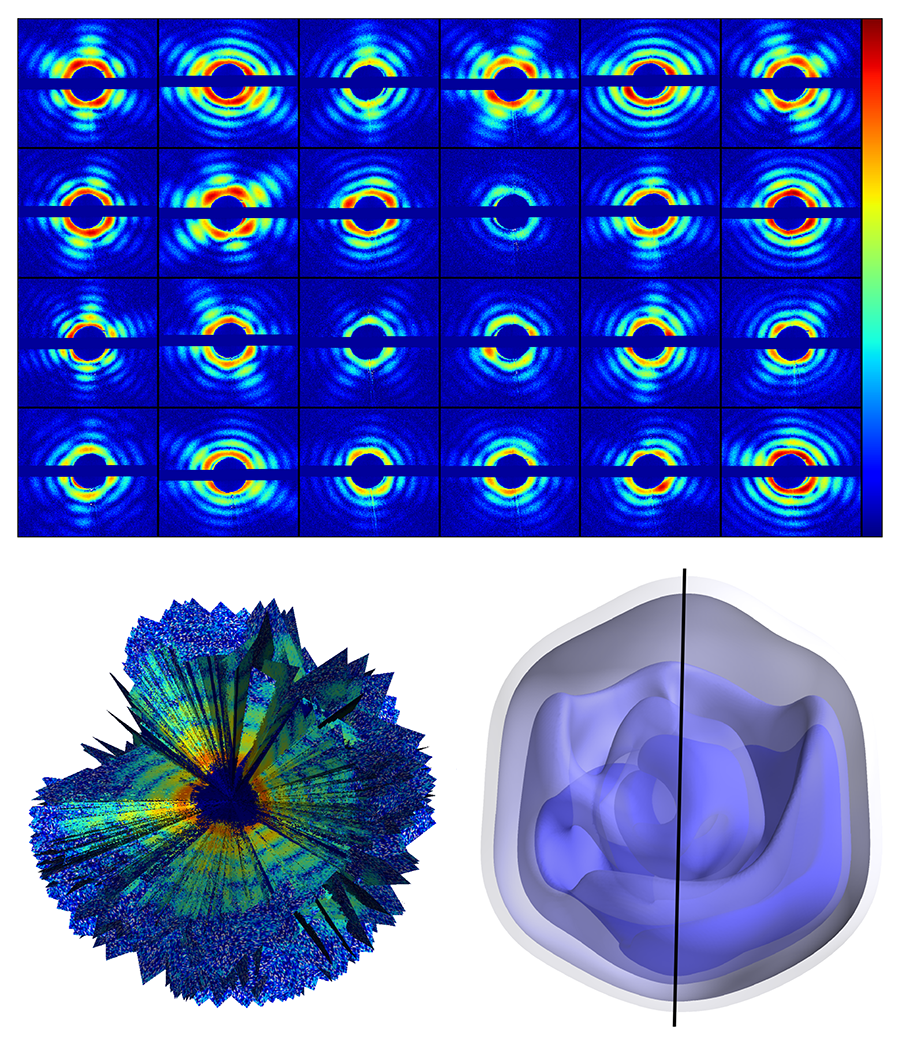
\includegraphics[width=0.5\textwidth]{Figuras/ch1_pulso.png}
  \caption{Patrones de difracción y densidad de electrones obtenida de un \enquote{Mimivirus}\autocite{Ekeberg2015}. La resolución conseguida es de \qty{125}{nm}. El tamaño de la envoltura del virus es aproximadamente de \qty{450}{nm}.}
  \label{fig:1.9}
\end{figure}

El aspecto clave del ancho de pulso en estas aplicaciones está en conseguir la difracción antes destruir completamente la muestra\autocite{Neutze2000} (ver Figura \ref{fig:1.10}), motivando la necesidad de pulsos extremadamente cortos o ultracortos ($\le\unit{fs}$) para visualizar imágenes. Por otro lado, el papel de la longitud de onda es conseguir la resolución necesaria para observar menores tamaños, ya que longitudes de onda mayores que el tamaño característico del objeto que quiere estudiarse no permiten exhiben el fenómeno de difracción necesario. En la actualidad ---se explicará más detalladamente en la sección \S\ref{sec:1.3}---, las únicas fuentes de radiación que reúnen estos requisitos son los láseres de rayos X blandos y los láseres de electrones libres.

\paragraph{Modos de Laguerre-Gauss}
Durante la sección \S\ref{sec:1.1.1}, emergió de forma natural el concepto de cavidad de Fabry-Perot o cavidad resonante. La función de estos sistemas ópticos es fundamental para conseguir una amplificación de la luz láser y, al mismo tiempo, permitir su salida después de penetrar a través del medio activo encargado de proporcionar el \enquote{sustrato} necesario para la emisión estimulada. La Figura \ref{fig:1.4} mostraba como, por ejemplo, una forma de liberar la luz láser consiste en utilizar espejos parcialmente transparentes a la frecuencia amplificada. Las sucesivas vueltas de los fotones atrapados en el interior de la cavidad consiguen multiplicar la energía liberada. 

\begin{figure}[htbp]
  \centering
  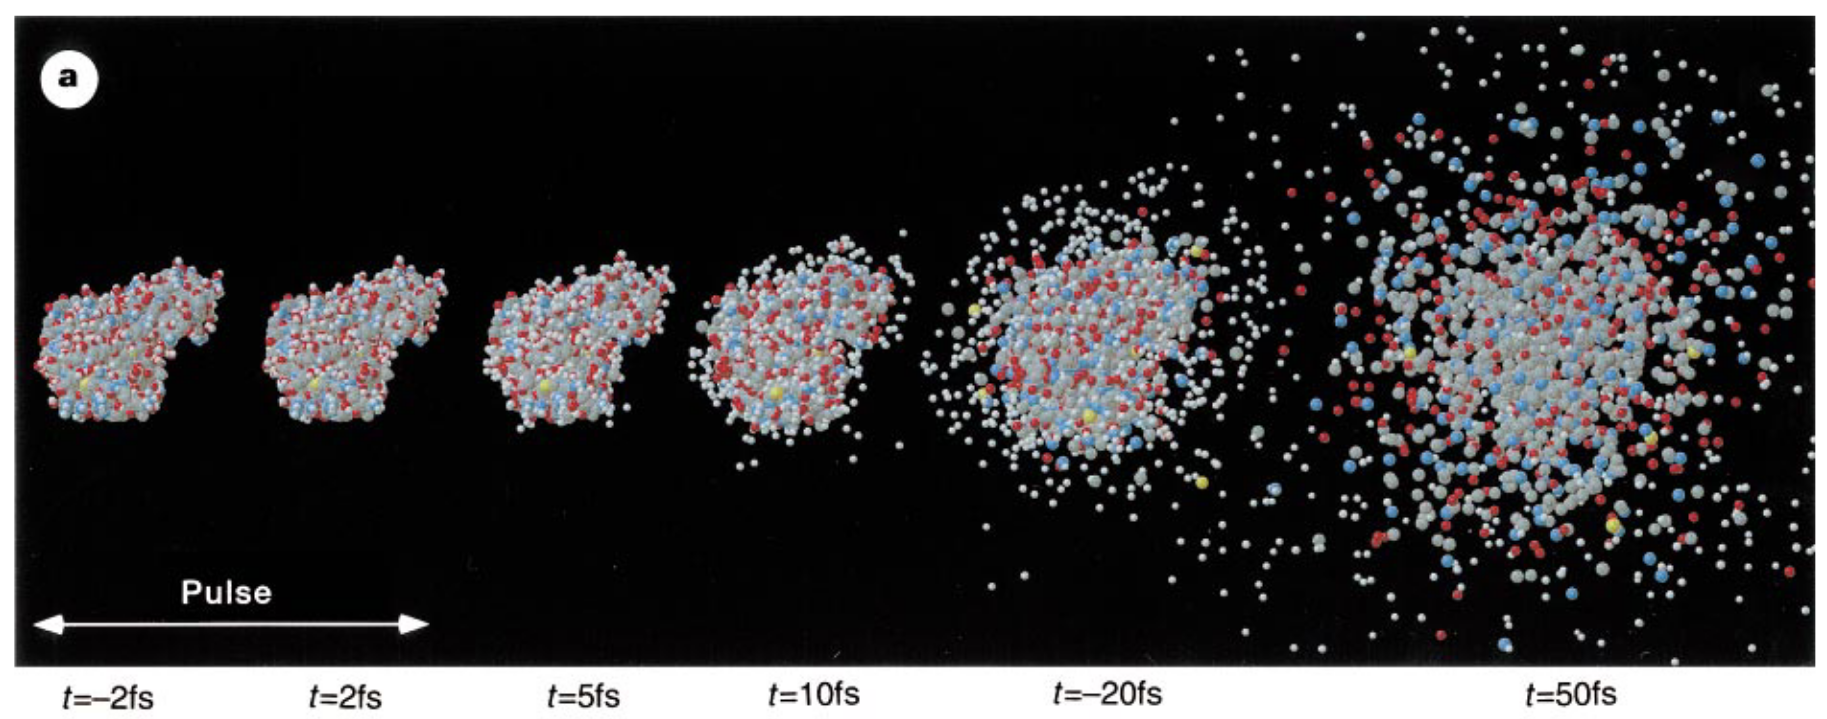
\includegraphics[width=0.8\textwidth]{Figuras/ch1_explyso}
  \caption{Explosión observada por Neutze \emph{et al} (2000) \autocite{Neutze2000} de la lisozima T4 (una proteína) tras recibir un pulso láser \acrshort{xuv} de $3 \times 10^{12}$ fotones por cada \qty{100}{nm} de diámetro, y un pulso con \acrshort{fwhm} de \qty{2}{fs}, provocando la desintegración de la enzima.}
  \label{fig:1.10}
\end{figure}

Por otro lado, la distancia entre ejes ópticos de la cavidad se escoge para obtener la ganancia deseada, acompañada de los elevados niveles de coherencia, direccionalidad y monocromaticidad típicos de un láser, favoreciendo la interferencia constructiva \autocite{Hecht2016} de los modos de vibración interesantes, centrados en torno a la frecuencia buscada. A raíz de esto, las propiedades ópticas del láser dependen considerablemente del diseño utilizado, prestando atención a la geometría de los espejos; la posición y tamaño de cavidad y medio activo; o a elementos con formas especiales colocados dentro de la cavidad, que permitan eliminar frecuencias de modos indeseados.

Estas cavidades, también pueden estudiarse mediante las condiciones de frontera externas impuestas sobre la propagación de la luz a través del espacio que llena el medio activo. Habitualmente, en física de láseres suele considerarse una cavidad \enquote{vacía} \autocite{Milonni1988}, esto es, no contiene materia, pero sí luz. Lógicamente, es una aproximación si la cavidad forma parte de un láser, pero es suficientemente precisa en muchas situaciones porque los átomos o moléculas del medio activo suelen rellenar las cavidades de manera muy dispersa. 

Bajo estas suposiciones, el campo eléctrico cumple la ecuación \eqref{eq:1.31} de ondas en el vacío 
\begin{equation}\label{eq:1.31}
  \laplacian \symbf{E} - \frac{1}{c^{2}}\pdvN{\symbf{E}}{t}{2} = 0,
\end{equation}
con solución una onda plana monocromática tipo $\symbf{E}(\symbf{r},t) = \symbf{E}_{0}(\symbf{r})\eu^{-\iu \omega t}$, dando lugar a la ecuación de Helmholtz $(\laplacian + k^{2}) \symbf{E}_{0} = 0$ para la amplitud (compleja) $\symbf{E}_{0}$ del campo eléctrico, siendo $k=\omega/c$ el número de onda. La dirección de propagación (escogiendo la dirección $z$) consiste en un término $\eu^{\iu kz}$ que puede incluirse dentro de la amplitud $\symbf{E}_{0}$, como $\symbf{E}_{0}(\symbf{r}) = \symbf{U}(\symbf{r})\eu^{\iu  kz}$. 

Utilizando la aproximación paraxial (que volverá a aparecer en la sección \S\ref{sec:3.1}), las variaciones de segundo orden de $\symbf{U}$ en la coordenada $z$ pueden suponerse despreciables frente a las de primer orden, cumpliéndose la ecuación \eqref{eq:1.32} de ondas paraxial
\begin{equation}\label{eq:1.32}
  \pdvN{\symbf{U}}{x}{2} + \pdvN{\symbf{U}}{y}{2} - 2 \iu k \pdv{\symbf{U}}{z} = 0,
\end{equation}
donde las diferentes soluciones, imponiendo unas condiciones de frontera determinadas, representan las posibles configuraciones del campo eléctrico en el plano perpendicular $xy$ a la dirección de propagación $z$, denominados \emph{modos transversales}.

Las soluciones $\symbf{U}$, a su vez, son desarrollos en serie de funciones conocidas como \emph{modos de Hermite-Gauss} $HG_{n,m}$ (también $\symrm{TEM}_{n,m}$, de \emph{transverse electromagnetic mode}), en coordenadas cartesianas, o \emph{modos de Laguerre-Gauss} $\symrm{LG}_{l,p}$ en coordenadas cilíndricas. Normalmente, para estudiar la distribución espacial (en un instante de tiempo) de un haz láser suelen utilizarse \emph{haces gaussianos}, que son sencillamente un caso particular de los modos transversales anteriores, con $n=m=l=p=0$. Este modo representa un campo eléctrico descrito por \autocite{Milonni1988}
\begin{align}
  \label{eq:1.33}
  \symrm{HG}_{0,0}=\symrm{LG}_{0,0}(r,z) &= E_{0}\frac{w_{0}}{w(z)}\frac{2r^{2}}{w^{2}(z)}\exp \left(-\frac{r^{2}}{w^{2}(z)}\right)\exp \left(-\iu kz - \iu \frac{kr^{2}}{2R(z)} + \iu \Phi(z)\right), \\
  \label{eq:1.34}
  w(z) &= w_{0}\sqrt{1+\left(\frac{z}{z_{R}}\right)^{2}}, \\
  \label{eq:1.35}
  R(z) &= z \left[1+\left(\frac{z_{R}}{z}\right)^{2}\right], \\
  \label{eq:1.36}
  \psi(z) &= \arctan\left(\frac{z}{z_{R}}\right),
\end{align}
donde $w_{0}$ es el valor mínimo del ancho del haz $w(z)$; $R(z)$ es el radio de curvatura del frente de onda; $\psi(z)$ es la \emph{fase de Gouy}, que consiste en un desplazamiento de la fase del haz gaussiano; y $z_{R}$ es el rango de Rayleigh, ya comentado durante la sección \S\ref{sec:1.1.2}. La forma típica de $w(z)$ aparece en la Figura \ref{fig:1.11}, junto a algunos de los parámetros característicos.

En general, los modos de Laguerre-Gauss, especialmente importantes cuando se incorpora un momento angular a los fotones del haz (estudiado al finalizar el capítulo \ref{cap:4}), pueden descomponerse y medirse (en un laboratorio) en función de los modos de Hermite-Gauss \autocite{DErrico2017} ($\symrm{TEM}_{n,m}$) y tienen una dependencia angular $\phi$ descrita por la ecuación 
\begin{equation}\label{eq:1.37}
  \begin{split} 
    \symrm{LG}_{l,p}(r,\phi,z) = E_{0}\frac{w_{0}}{w(z)}L_{p}^{(l)} \left(\frac{\sqrt{2}r}{w(z)}\right)^{|l|}\frac{2r^{2}}{w^{2}(z)}&\exp \left(-\frac{r^{2}}{w^{2}(z)}\right)\times \\ 
    & \exp \left(- \iu \phi l - \iu \frac{kr^{2}}{2R(z)} + \iu \Phi(z)\right),
  \end{split}
\end{equation}
con $L_{p}^{|l|}$ los \emph{polinomios de Laguerre}
\begin{equation}\label{eq:1.38}
  L_{p}^{|l|}(x) = \sum_{m=0}^{p}(-1)^{m}\frac{(|l|+p)!}{(p-m)!(|l|+m)!m!}x^{m}.
\end{equation}

\begin{figure}[htbp]
  \centering
  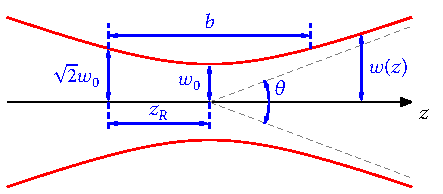
\includegraphics[width=0.7\textwidth]{Figuras/ch1_beam_waist.pdf}
  \caption{Ángulo de divergencia $\theta$ del ancho del haz láser $w(z)$ con la longitud $z$, rango de Rayleigh $z_{R}$, y ancho inicial $w_{0}$. Obsérvese que, para $z=z_{R}$, el ancho del haz aumenta en un factor $\sqrt{2}$.}
  \label{fig:1.11}
\end{figure}

Analizando la ecuación \eqref{eq:1.37}, el modo de Laguerre-Gauss $\symrm{LG}_{l,p}$ es muy similar al modo fundamental de Hermite-Gauss $\symrm{TEM}_{0,0}$ (y a su propio modo fundamental) que representa un haz gaussiano, añadiendo la dependencia angular exponencial $\exp(-\iu \phi l)$, los polinomios de Laguerre, y el término potencia elevado a $|l|$. Los subíndices $p$ y $l$ contienen el comportamiento radial y angular, respectivamente. El índice radial $p$ está directamente relacionado con el número de anillos concéntricos que aparecen en la sección transversal del haz, de manera que habrá $p+1$ anillos cuando $l\neq 0$ y $p$ anillos cuando $l=0$, como ilustran los ejemplos en la Figura \ref{fig:1.12}. 

\begin{figure}[htbp]
  \centering
  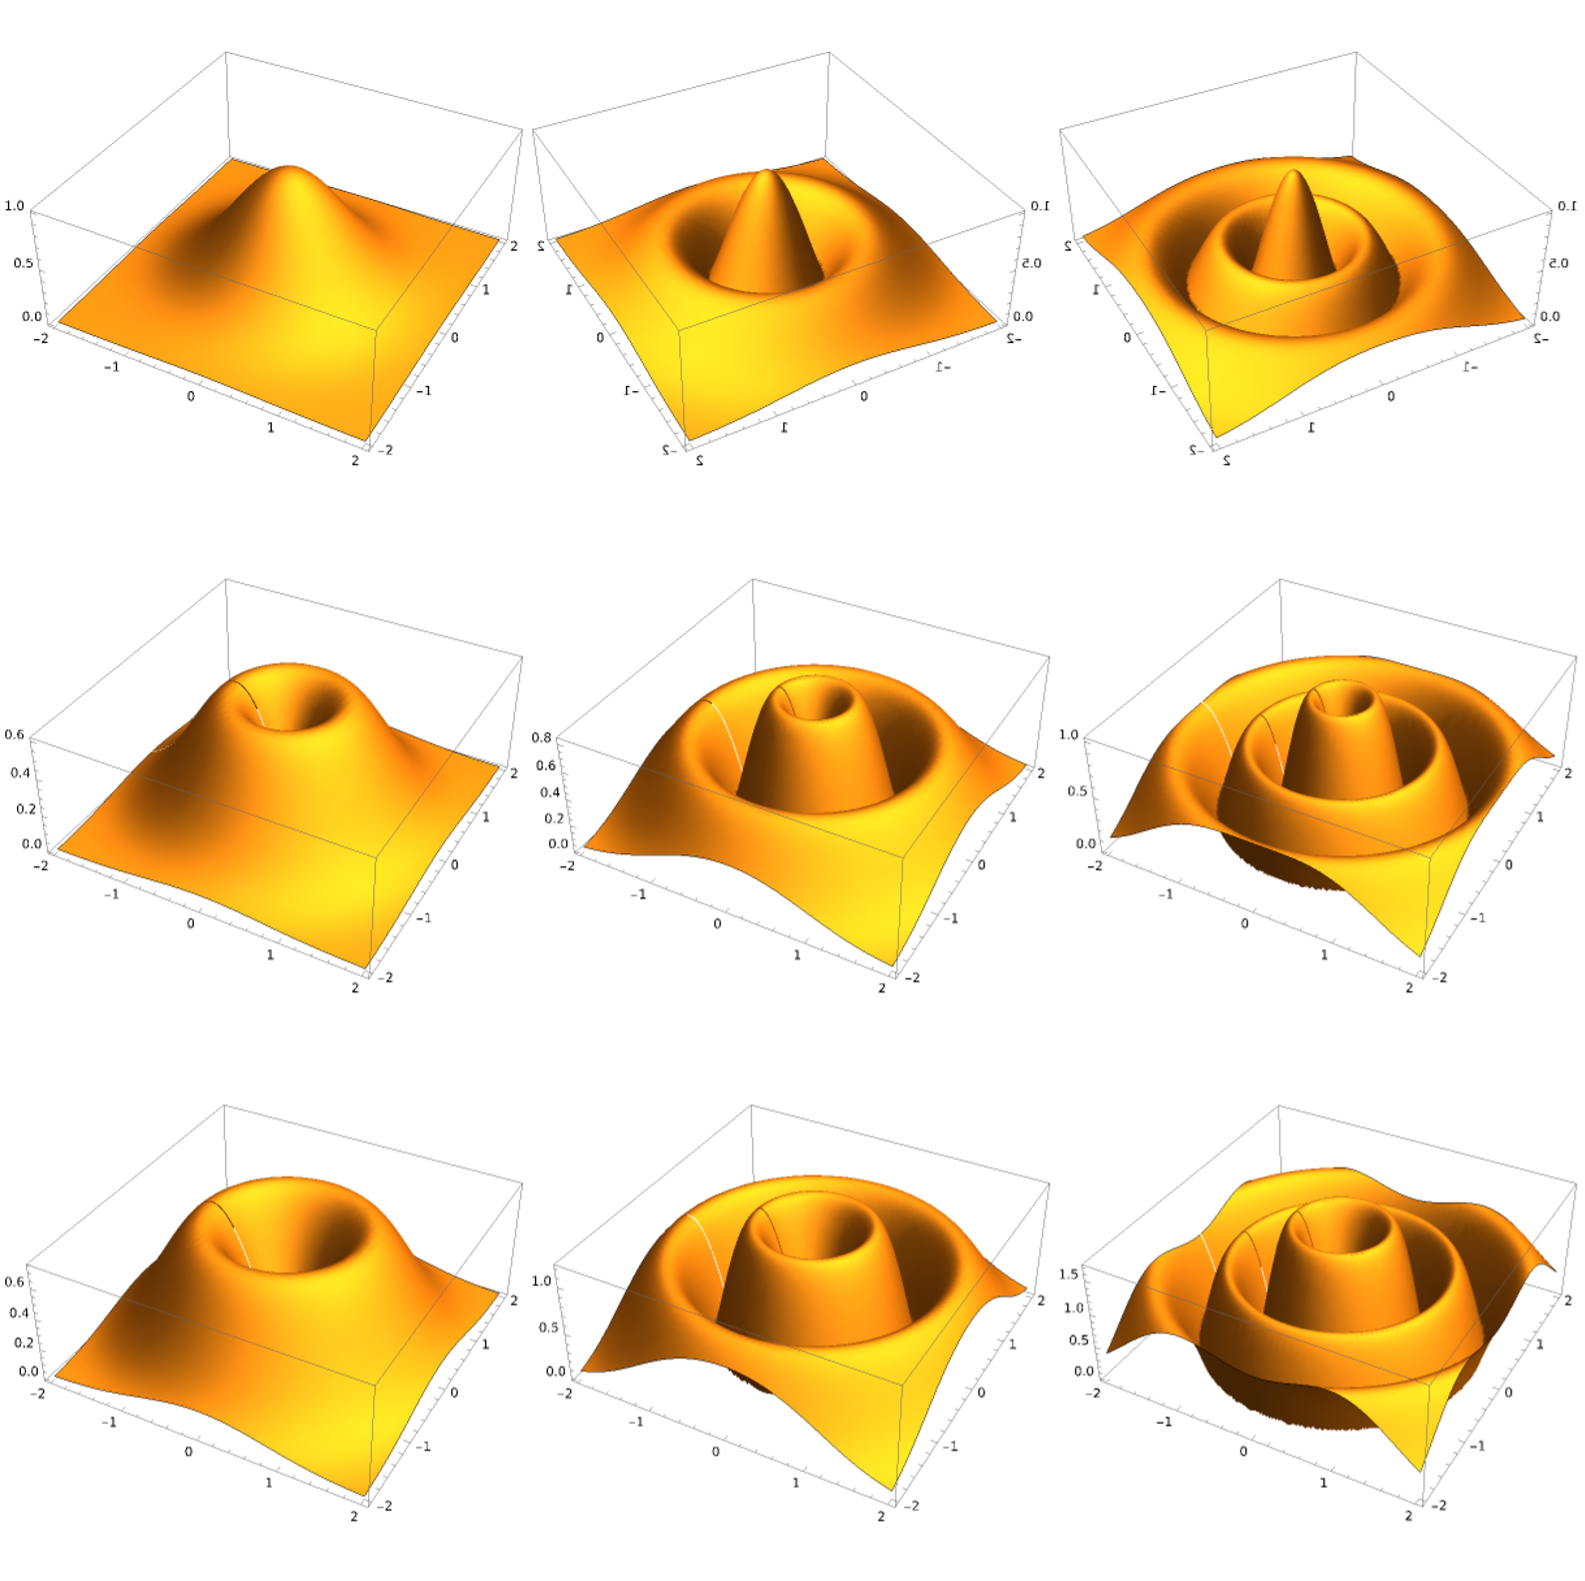
\includegraphics[width=0.5\textwidth]{Figuras/ch1_lague_gauss.png}
  \caption{Ejemplos de modos de Laguerre-Gauss. De izquierda a derecha, índices $p=0$ hasta $p=2$, y de arriba a abajo, índices $l=0$ hasta $l=2$. La intensidad de los colores representa la magnitud del valor tomado por el modo.}
  \label{fig:1.12}
\end{figure}

El índice angular $l$, tiene tres nombres, algunos de origen matemático: \autocite{Yao2011} \emph{\acrfull{tc}} (carga topológica, el más común), \emph{winding number} (número de vueltas) o \emph{dislocation strength} (dislocación en tornillo). Este número concede al frente de onda del campo eléctrico una trayectoria helicoidal en su dirección de propagación $z$, su valor determina el número de vueltas o hélices formadas en un periodo de amplitud $2 \pi$, y su signo proporciona el sentido de giro. Esencialmente, el subíndice $l$ es el número de veces que la luz se \enquote{retuerce} al recorrer una longitud de onda. El momento angular aportado a los fotones (en la última parte del capítulo \ref{cap:4}) es consecuencia de este \enquote{alabeo} del frente de onda, apareciendo representada espacialmente la evolución de la fase en la Figura \ref{fig:1.13}.

Estos rayos de luz son conocidos como \enquote{vórtices ópticos} ---del acrónimo \emph{\acrfull{ov}}---, y están caracterizados por una \enquote{singularidad} en su centro, donde las ecuaciones que describen el comportamiento de la onda no tienen solución, pues la fase del frente de onda no está definida y la intensidad es nula, como muestran las Figuras \ref{fig:1.12} y \ref{fig:1.13}. Es un punto donde el modo de Laguerre-Gauss correspondiente no cumple con las condiciones de continuidad y derivabilidad necesarias para formar parte del espacio de soluciones de la ecuación \eqref{eq:1.32}.

En concreto, el concepto de vórtice óptico apareció originalmente \autocite{Shen2019} porque el vector de Poynting (flujo de energía de la luz) gira en el límite del centro del vórtice a velocidad infinita, anulándose la intensidad. La singularidad óptica también puede entenderse como aquel punto donde la fase se repite cada $2 \pi/l$ radianes, provocando un patrón de interferencia destructiva entre las $2l$ parejas de valores iguales de la fase que confluyen en el centro, provocando la anulación de la intensidad en dicho punto. En este sentido, el responsable de este fenómeno es el término $\exp(-\iu l \phi)$, que tiene un periodo de $2 \pi/l$ radianes, originando el patrón de repetición de la fase en torno a la singularidad.

\begin{figure}[htbp]
  \centering
  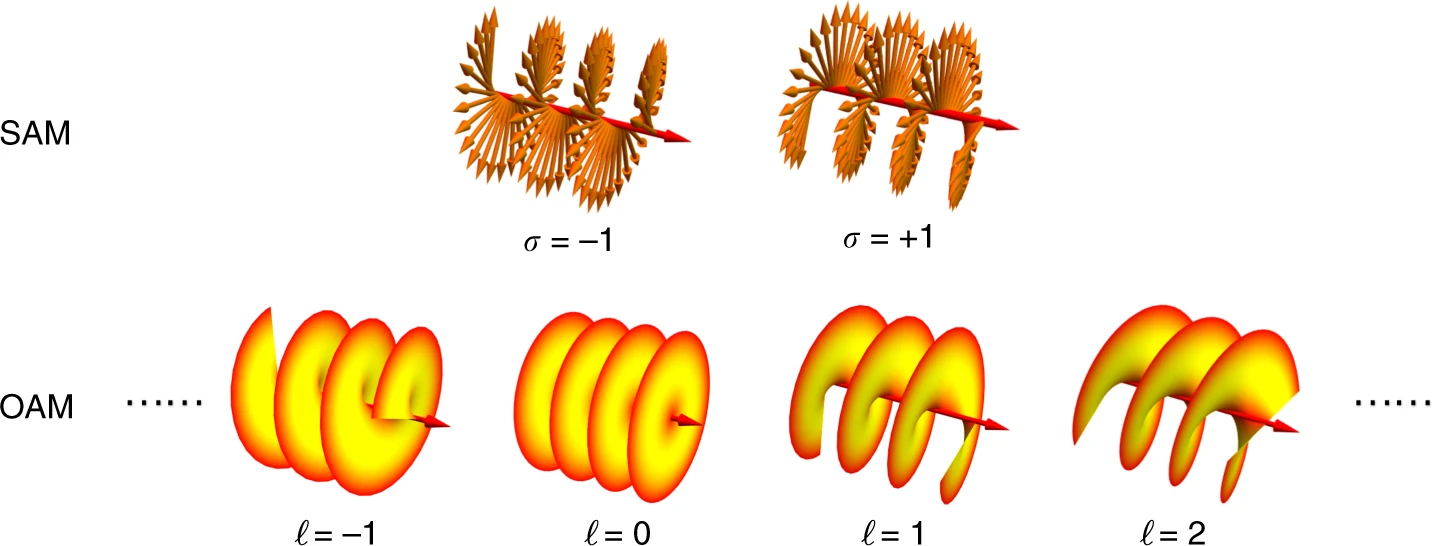
\includegraphics[width=0.85\textwidth]{Figuras/ch1_oam_sam.png}
  \caption{Distribución de la fase para distintos estados $l$ del haz, proporcionando un momento angular orbital al haz, y para distintos estados $\pm \sigma$ de polarización, responsable del momento angular de espín \autocite{Shen2019}.}
  \label{fig:1.13}
\end{figure}

Una pregunta razonable que podría hacerse es: ¿cómo pueden generarse pulsos con estas características? El esquema básico consiste en hacer pasar una onda plana a través de un sistema óptico conocido como \emph{\acrfull{spp}} (disco de fase espiral) \autocite{Yao2011}, formado por un disco óptico de ancho óptico variable $s$ con el ángulo $\phi$ tal que $s \propto l \lambda \phi/\symfrak{n}$ (la superficie es helicoidal), con $\symfrak{n}$ el índice de refracción del disco óptico. En la refracción a la salida de la superficie helicoidal, el momento lineal del fotón adquiere una componente angular, dando lugar al momento angular alrededor del eje óptico de disco. 

El problema de este sistema es que la geometría del disco es extremadamente compleja de fabricar, especialmente para las longitudes de onda en el rango óptico. En lugar de utilizar la refracción de la luz, es posible utilizar \emph{rejillas de difracción} o \emph{lentes de Fresnel} como \enquote{hologramas} del elemento óptico deseado, \autocite{Yao2011} con una geometría que consiga el mismos resultado que la refracción del SPP, aunque los modos de Laguerre-Gauss fundamentales no pueden reproducirse con precisión.

\paragraph{Momento angular orbital}
Aunque el objetivo del presente trabajo, como aparecerá en el próximo capítulo \S\ref{cap:2}, no consiste en estudiar las propiedades de pulsos láser con momento angular (excepto una última parte de las simulaciones del capítulo \S\ref{cap:4}), es interesante proporcionar unas nociones básicas de por qué los fotones tienen momento angular, qué significa, y por qué los modos de Laguerre-Gauss describen haces con esta propiedad. Un desarrollo más profundo, exhaustivo y detallado puede encontrarse en Allen (1999)\autocite{Allen1999}.

Desde que Louis de Broglie propuso, entre $1923$\autocite{deBroglie1923} y $1924$\autocite{deBroglie1924}, el comportamiento de los electrones y, en general, las partículas como \enquote{ondas de materia}, es conocido que la luz transporta no solo energía, sino también una cantidad de movimiento o momento lineal $p = h/\lambda$. En cambio, el momento angular de la luz no recibió en aquella época la misma atención que el momento lineal, a pesar de que más de una década antes, John Henry Poynting \autocite{Poynting1909} (el mismo físico al que debe su nombre el vector de Poynting) ya había explorado sus fundamentos y propuesto la relación entre polarización y momento angular. 

Sin embargo, es cierto que a principios del siglo \RN{20} la hipótesis propuesta por de Broglie tuvo confirmación experimental muy pocos años después, en el experimento de Davisson y Germer de $1927$ \autocite{Davisson1927} con la observación de la difracción de electrones en un cristal de níquel, mientras que la observación de momento angular en partículas en fotones tardó más tiempo en llegar, en $1936$, con un dispositivo mecánico desarrollado por el físico Richard A. Beth \autocite{Beth1936}.

El momento angular de cualquier sistema físico puede descomponerse en dos partes: el conocido momento angular orbital o \emph{\acrfull{oam}}, y el momento angular de espín o \emph{\acrfull{sam}}. Un ejemplo clásico \autocite{Tipler2021b} es la órbita de la Tierra alrededor del Sol. La Tierra tiene un momento angular orbital $\symbf{L}$ respecto del centro del Sol debido a su movimiento orbital alrededor de éste y un momento angular de espín $\symbf{S}$ debido al movimiento de rotación alrededor de su eje de rotación. La suma de ambos proporciona el momento angular total del sistema $\symbf{J} = \symbf{L} + \symbf{S}$, de manera que el movimiento de traslación terrestre es consecuencia del momento angular orbital y el movimiento de rotación del momento angular de espín.

Los fotones son partículas puntuales sin masa (en reposo), así que estos conceptos clásicos aplicados a la luz necesitan intuiciones distintas y nuevos puntos de vista. En la teoría electromagnética de Maxwell, los fotones tienen momento angular orbital debido a su distribución espacial (de la intensidad y la fase) \autocite{Jackson1998} y momento angular de espín debido a la polarización del campo eléctrico, como demostró Beth \autocite{Beth1936} durante el experimento. El intercambio de fotones con momento lineal $p$ y una superficie opaca, por ejemplo, un bloque de hormigón pintado de negro, produciría una fuerza neta capaz de empujarlo (evidentemente es una fuerza despreciable para un bloque de hormigón, pero ¿y si fuesen átomos? \autocite{Ashkin1970,Ashkin1978}) debido a la conservación de la cantidad de movimiento.

A esta fuerza, la llamada \emph{presión de radiación} de la luz, podría asociarse un par de fuerzas capaz de hacer girar las puertas giratorias de cualquier edificio público. Por otro lado, el momento angular de espín podría interpretarse como un movimiento de giro \enquote{intrínseco} capaz de girar la llave de un cajón, aunque la única condición para conseguir esto sería que la luz estuviese polarizada circularmente \autocite{Beth1936}.

La observación y medición del momento angular (de espín) de la luz realizada por Beth\autocite{Beth1936} empleaba la idea propuesta por Poynting \autocite{Poynting1909} de que, de manera similar al intercambio de momento lineal $p$ de los fotones con un cuerpo opaco, un intercambio de momento angular $\symbf{J}$ con un sistema óptico (por conservación del momento angular) debía provocar un cambio del estado de polarización circular (dextrógiro a levógiro, o viceversa) de los fotones. Técnicamente, Beth midió el par mecánico ejercido por un haz de luz sobre un disco birrefringente de cuarzo (como muestra la Figura \ref{fig:1.14}), verificando las predicciones de la teoría cuántica para el espín de $\pm \hslash $ con polarización a izquierda y derecha.

\begin{figure}[htbp]
  \centering
  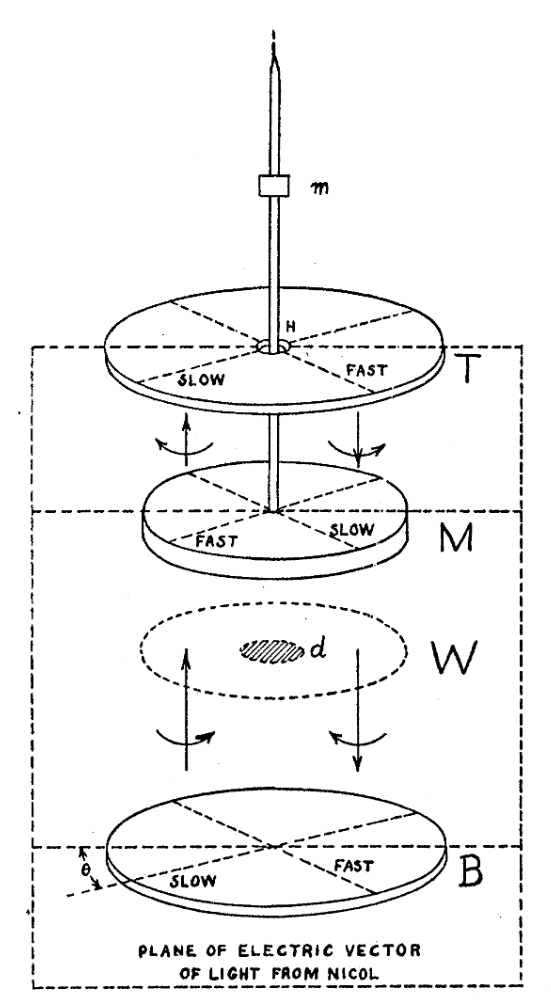
\includegraphics[width=0.26\textwidth]{Figuras/ch1_quartz_plate.png}
  \caption{Montaje de los platos de cuarzo utilizados por Beth. \autocite{Beth1936}}
  \label{fig:1.14}
\end{figure}

Medio siglo más tarde, en 1992, L. Allen \emph{et al} demostraron \autocite{Allen1992} que el término $\exp(-il \phi)$ en los modos de Laguerre-Gauss de la ecuación \eqref{eq:1.37} albergan un \acrshort{oam} propio en ocasiones superior (de hecho, en un factor $l$) que el \acrshort{sam}, de acuerdo con la analogía entre mecánica cuántica y la óptica paraxial \autocite{Born2019} de que, estos modos se corresponden con los autovalores $\pm l \hslash $ del operador momento angular $L_{z}$, tal que $L_{z}u= -\iu \hslash \pdiff_{\phi}u=\pm l \hslash u$. El experimento que propusieron sigue la misma línea que Beth, pero sustituyendo los discos de cuarzo por parejas de lentes cilíndricas.

El campo $u=u(r,\phi,z)$ sobre el que actúa el operador $L_{z}$ podría ser, por ejemplo, cualquiera de los modos de Laguerre-Gauss. Estos modos, en general, pueden escribirse en coordenadas cilíndricas como $u(r,\phi,z) = u_{0}(r,z)\exp(-\iu l \phi)$, que cumplen la ecuación de ondas paraxial \eqref{eq:1.32}. Con esta aproximación, la componente angular del momento lineal $p_{\phi}$ (la densidad de momento) coincide con la parte real vector de Poynting (su componente angular), $p_{\phi} = \epsilon_{0}\langle\symbf{E}\times \symbf{B}\rangle_{\phi}$, promediado en el tiempo. La ecuación completa para la densidad de momento lineal toma la forma
\begin{equation}\label{eq:1.38}
  \symbf{p} = \epsilon_{0}\langle\symbf{E}\times \symbf{B}\rangle = \frac{\epsilon_{0}}{2}(\symbf{E}^{*}\times \symbf{B} + \symbf{E}\times \symbf{B}^{*}) = \iu \omega \frac{\epsilon_{0}}{2} (u^{*}\grad u - u \grad u^{*}) + \epsilon_{0} \omega k |u|^{2}\unitvector_{z},
\end{equation}
con $k$ el número de onda y $\symbf{e}_{z}$ un vector unitario en la dirección $z$. Desarrollando las componentes de la ecuación \eqref{eq:1.38}, la parte angular de la densidad de momento lineal queda $p_{\phi}=\epsilon_{0} \omega l |u|^{2}/r$, que proporciona el momento angular total de la luz. La componente según $z$ del momento angular $j_{z}$ (esta vez densidad de momento angular) puede calcularse directamente tomando el producto vectorial
\begin{equation}\label{eq:1.39}
  \symbf{j}_{z} = \symbf{r}\times \symbf{p}_{\phi} = \epsilon_{0} \omega l |u|^{2}\unitvector_{z}.
\end{equation}
Por otro lado, la densidad de energía del campo electromagnético es $w = c \epsilon_{0}\xval{\symbf{E}\times \symbf{B}}_{z} = \epsilon_{0} \omega^{2} |u|^{2}$, es decir, el producto de la velocidad de la luz en el vacío y la densidad de momento lineal, por tanto
\begin{equation}\label{eq:.1.40}
  \frac{j_{z}}{w} = \frac{l}{\omega}.
\end{equation}
Si ambas densidad de energía y momento angular son integradas en el plano $xy$, la relación entre el momento angular y la densidad de energía de un haz (ambos por unidad de longitud tras la integración) es
\begin{equation}\label{eq:1.41}
  \frac{\iint(r \times \xval{\symbf{E}\times \symbf{B}})_{z}\, r\!\diff r\!\diff \phi}{\iint \xval{\symbf{E}\times \symbf{B}}_{z}\, r\!\diff r\!\diff \phi} = \frac{l}{\omega}.
\end{equation}
Comparando las componentes según $z$ de las densidades de momento lineal y angular, utilizando las ecuaciones \eqref{eq:1.38} y \eqref{eq:1.39}, resulta que $p_{z}/j_{z}=\omega l /\omega k = l \lambda/2 \pi$, demostrando que el haz tiene un momento angular orbital $l$ por cada fotón, y que no tiene su origen en el momento angular de espín. La ecuación \eqref{eq:1.41} es el equivalente para el momento angular orbital de la relación entre el momento angular de espín y la energía, $\pm \hslash /\hslash \omega = \pm 1/\omega$, para luz polarizada circularmente

Intuitivamente, el término $\exp(- \iu l \phi)$ causante de la aparición del \acrshort{oam} describe una superficie bidimensional formada por un hiperboloide de una hoja, como muestra el frente de onda en la Figura \ref{fig:1.15}. La superficie es consecuencia del campo vectorial formado por el vector de Poynting, esto es, la densidad del flujo de energía del haz, que \enquote{desliza} tangencialmente sobre el hiperboloide de revolución. La orientación del eje hiperboloide (la directriz) tiene la dirección marcada por las componentes axiales del campo eléctrico y magnético, que son paralelas a dicho eje, mientras que las componentes transversales de ambos campos (paralelas al vector normal de la superficie) determinan la forma del hiperboloide. Es una forma geométrica de entender la aparición del \acrshort{oam} en la luz.

\begin{figure}[htbp]
  \centering
  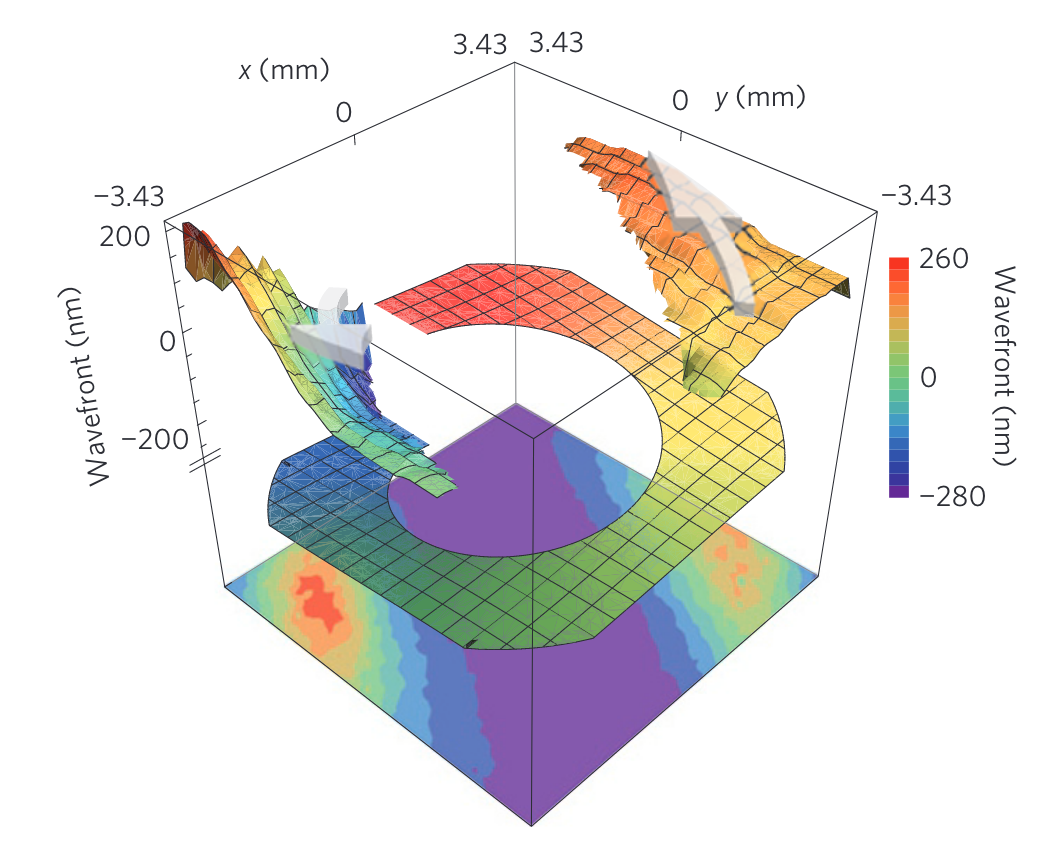
\includegraphics[width=0.4\textwidth]{Figuras/ch1_helicoidal.png}
  \caption{Medición del frente de onda helicoidal de un vórtice óptico realizada por Zürch \emph{et al} (2012)\autocite{Zurch2012}.}
  \label{fig:1.15}
\end{figure}

En el caso de una polarización circular, con $\sigma = \pm 1$ (ver Figura \ref{fig:1.13}), o $\sigma = 0$ para la polarización lineal, la ecuación \eqref{eq:1.41} se transforma en
\begin{equation}\label{eq:1.42}
  \frac{\iint(r \times \xval{\symbf{E}\times \symbf{B}})_{z}\, r\!\diff r\!\diff \phi}{\iint \xval{\symbf{E}\times \symbf{B}}_{z}\, r\!\diff r\!\diff \phi} = \frac{l + \sigma}{\omega},
\end{equation}
resultado válido más allá de la aproximación paraxial utilizada, para cualquier potencial vector utilizado para generar la solución de las ecuaciones de Maxwell \autocite{Barnett1994}. La obtención de la ecuación \eqref{eq:1.42} es mucho más compleja que la anterior ecuación \eqref{eq:1.41} porque \autocite{Barnett2001} fuera de la solución paraxial, y en general, para geometrías más complejas, la identificación de la parte orbital y de espín del momento angular no es tan sencilla. Normalmente, por ejemplo, Barnett (2001) \autocite{Barnett2001} propuso y demostró la posibilidad de emplear formulaciones invariantes bajo transformaciones de Lorentz que puedan extenderse a la electrodinámica cuántica para obtener este resultado.

Además, recordando que el campo $u(r,\phi,z)$ puede ser cualquiera de los modos de Laguerre-Gauss $\symrm{LG}_{l,p}$, este análisis demuestra que los haces formados por estos modos tienen un \acrshort{oam} propio, independiente del \acrshort{sam}. Actualmente, pueden generarse otros modos con frentes de onda helicoidales, como los de Ince-Gauss, Bessel, Mathieu o geométricos $\symrm{SU(2)}$ que, también poseen \acrshort{oam}. Escogiendo los modos de Laguerre-Gauss de la ecuación \eqref{eq:1.37} y sustituyéndolos en la ecuación \eqref{eq:1.38}, resulta que su densidad de momento lineal es
\begin{equation}\label{eq:1.43}
  \symbf{p} = \epsilon_{0} \left(\frac{\omega k r z}{z^{2}+z_{R}^{2}}\unitvector_{r}+\frac{wl}{r}\unitvector_{\phi}+wl \unitvector_{z}\right)|\symrm{LG_{l,p}}|^{2},
\end{equation}
con $z_{R}$ el rango de Rayleigh. Tomando el producto vectorial con el vector de posición $\symbf{r}$, la densidad de momento angular es
\begin{equation}\label{eq:1.44}
  \symbf{j} = \symbf{r} \times \symbf{p} = \epsilon_{0} \left(-\frac{\omega l z}{r}\unitvector_{r}-wkr \left(\frac{z_{R}^{2}}{z^{2}+z_{R}^{2}}\right)\unitvector_{\phi}+wl \unitvector_{z}\right)|\symrm{LG_{l,p}|^{2}}.
\end{equation}

La ventaja de utilizar el vector de Poynting en esta descripción del \acrshort{oam} está en que, como se ha explicado, este campo vectorial representa la densidad del flujo de energía de la luz \autocite{Griffiths2017,Jackson1998}, cuyas líneas de campo se \enquote{arremolinan} siguiendo la dirección de propagación del haz. Además, la velocidad de rotación descrita es proporcional \autocite{Padgett1995} a la fase de Gouy presentada anteriormente en la ecuación \eqref{eq:1.36}, de forma que para el modo $p=0$ no depende del índice angular $l$, realizando una vuelta completa para el radio de máxima intensidad $r_{\mathrm{max, I}}(z)=\sqrt{w(z)l/2}$.

Mencionar que la construcción del equipo que soportaba las lentes cilíndricas para medir el \acrshort{oam}, como propusieron Allen \emph{et al} (1992) \autocite{Allen1992}, nunca se realizó porque resultó ser imposible con los medios que disponían. La demostración experimental y medición del \acrshort{oam} la realizaron He \emph{et al} (1995) \autocite{He1995,Friese1996}, induciendo una rotación en partículas de \ce{CuO} de entre \qty{1}{µm} y \qty{5}{µm} de diámetro mediante la transferencia del \acrshort{oam} de un haz láser \ce{He-Ne} a \qty{632.8}{nm}. Las frecuencias de giro conseguidas alcanzaron los \qty{10}{Hz} (dependiendo de la forma de las partículas), proporcionando otra analogía \autocite{Simpson1997} con la mecánica clásica entre el \acrshort{sam} y \acrshort{oam}.

Hace 34 años, Coullet \emph{et al} (1989) \autocite{Coullet1989} propuso un símil entre las singularidades ópticas (que denominó \emph{vórtices ópticos}) observadas en las cavidades resonantes de los láseres con los vórtices característicos en hidrodinámica de fluidos. Estos haces láser han resultado tener una conexión más profunda entre el mundo macroscópico de la óptica física y el mundo microscópico de la óptica cuántica. Estas propiedades han proporcionado una mayor comprensión de fenómenos como el acoplamiento espín-órbita \autocite{Dorney2019,Bliokh2015}, estructuras plasmónicas\autocite{Zhang2018}, generación de armónicos de alto orden (\acrshort{hhg})\autocite{Zurch2012,Dorney2019,Gui2021}, condensados de Bose-Einstein \autocite{Aranson2002}, etc.

Sus aplicaciones han alcanzado campos tan dispares como la codificación, procesamiento y transmisión de información, por ejemplo, en computación y tecnologías cuánticas \autocite{Erhard2018}; empleando fotones con estados entrelazados; en comunicaciones ópticas, consiguiendo enviar grandes cantidades de datos, del orden de $\qty{1}{Tbit/s}$, mediante la modulación multinivel de la amplitud y fase de la luz con \acrshort{oam} \autocite{Wang2012}; en la formación y reconstrucción de imágenes, obteniendo hologramas de muy alta resolución, capacidad y calidad\autocite{Shi2023}; en astrofísica, para el estudio de agujeros negros en rotación, los agujeros negros de Kerr, \autocite{Tamburini2011} a partir del \acrshort{oam} \enquote{impreso} en la luz que viaja cerca de ellos; o en bioquímica y biomedicina, para manipular y ensamblar proteínas o moléculas complejas como, por ejemplo, el ADN \autocite{Zhuang2004}. La luz en su máximo esplendor está por llegar, como muestra la Figura \ref{fig:1.16}.

\begin{figure}[htbp]
  \centering
  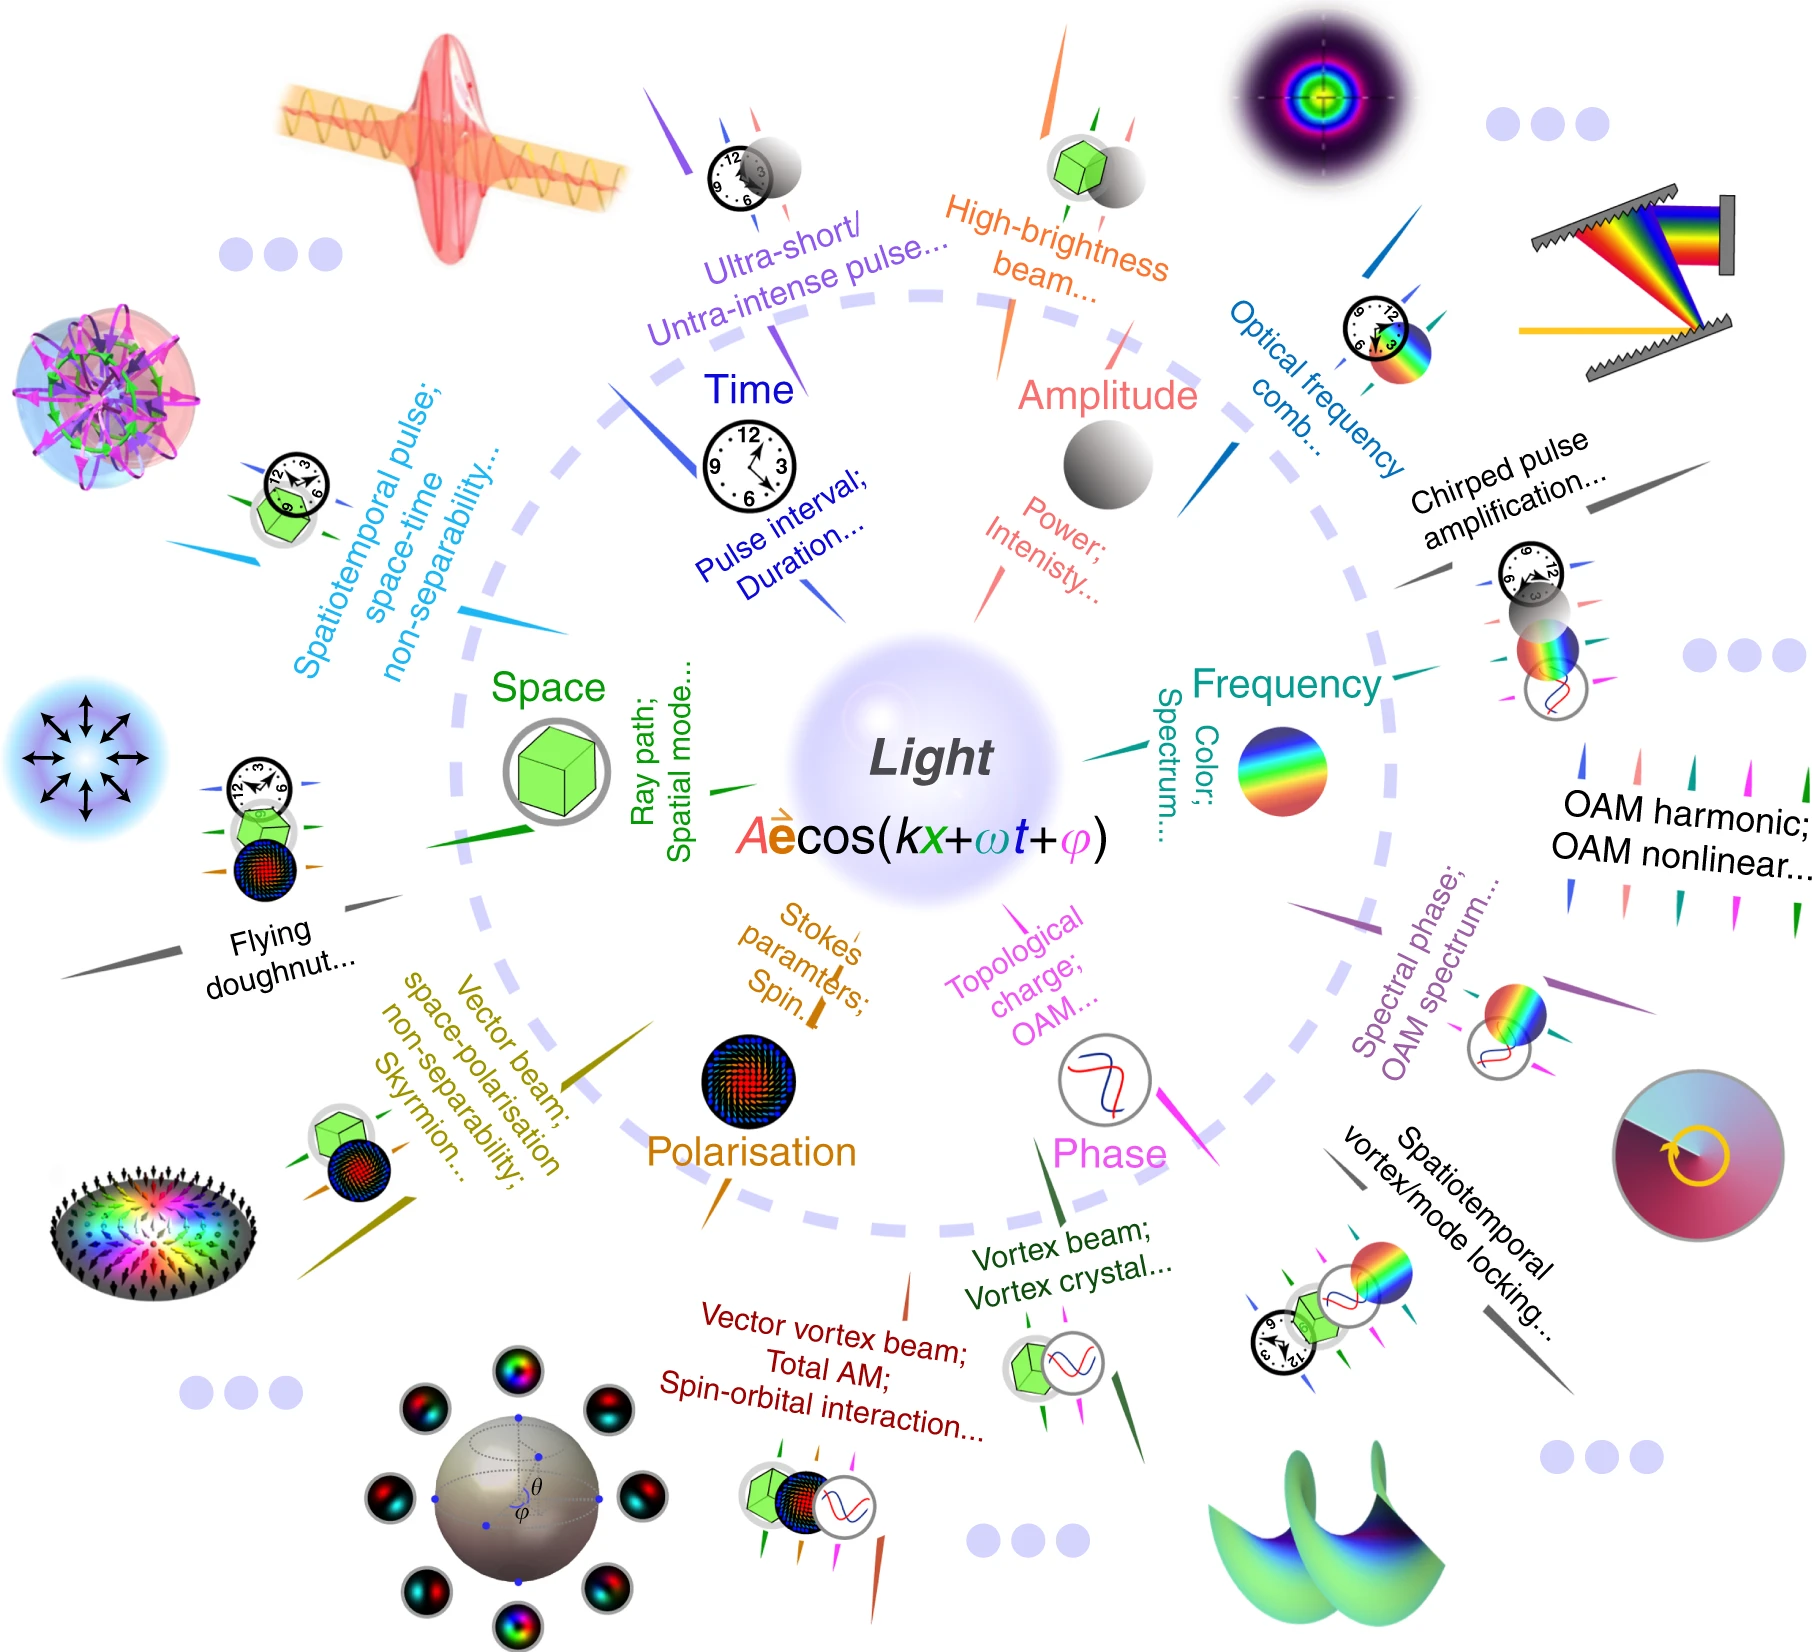
\includegraphics[width=0.7\textwidth]{Figuras/ch1_app_oam.png}
  \caption{Aplicaciones y perspectivas de la luz en distintos ámbitos y áreas de investigación \autocite{He2022}.}
  \label{fig:1.16}
\end{figure}

\section{Plasma}\label{sec:1.2}
El medio activo encargado en este trabajo de lograr la amplificación láser deseada consiste en un plasma y, puesto que es un estado de la materia muy particular en relación con la luz y su propagación a través de este, esta sección \S\ref{sec:1.2} prestará atención brevemente a los aspectos fundamentales que resultan interesantes para comprender esta interacción láser-plasma. 

Un plasma consiste en un gas altamente ionizado (mediante, por ejemplo, calentamiento), formado entonces por electrones e iones, y que tienen una densidad suficientemente baja para poder estudiarse dentro del marco de la física clásica (las partículas siguen una estadística de Maxwell-Boltzmann, en lugar de las estadísticas cuánticas de Fermi-Dirac o Bose-Einstein)\autocite{Thorne2017}. Su presencia en diversos campos de la ciencia y la tecnología ha ido en aumento desde la década de 1950, durante el desarrollo del programa de fusión termonuclear controlada (y, también, de la bomba termonuclear), pasando por la radioastronomía y el estudio de objetos astronómicos extragalácticos como cuásares y púlsares.

Estudiar el comportamiento de un plasma es más complejo que en la mayoría de sólidos, líquidos y gases principalmente por dos motivos:

\begin{enumerate}[label=(\roman*)]

    \item La dispersión Coulombiana entre partículas cargadas en un plasma es extremadamente débil, haciendo que los recorridos medios de las partículas libres sean superiores que el tamaño macroscópico del plasma, introduciendo fuertes anisotropías en las magnitudes dinámicas que describen dichas partículas.

    \item La interacción electromagnética entre las partículas cargadas en un plasma es de largo alcance, dando lugar a \enquote{acoplamientos} entre estas partículas y formando modos de vibración, es decir, ondas en el plasma, que se comportan como entidades físicas propiamente dichas.

\end{enumerate}

Una manera de acercarse a entender (de forma breve) este estado de la materia es través de los parámetros fundamentales que distinguen un plasma de los demás estados de la materia, que presenta la sección \S\ref{sec:1.2.1}. Después, la sección \S\ref{sec:1.2.2} estará dedicada a obtener la ecuación de ondas para el campo eléctrico a través del plasma, necesaria para estudiar la amplificación y propagación de un haz láser, como mostrará la sección \S\ref{sec:3.1}.

\subsection{Parámetros físicos}\label{sec:1.2.1}
Sin pérdida de generalidad, puede suponerse un plasma formado por el mismo número de especies cargadas positivamente (iones), con masa $m_{i}$ y carga $e$, y electrones con masa $m_{e}$ y carga $-e$ (con $e$ la carga eléctrica del electrón). Entonces, la energía cinética media de cualquier especie $s$ puede expresarse como la \emph{temperatura cinética} \autocite{Fitzpatrick2022}
\begin{equation}\label{eq:1.45}
  T_{s} = \frac{1}{3}m_{s}\xval{v_{s}^{2}},
\end{equation}
donde $\xval{v_{s}^{2}}$ es el valor medio de las velocidades para el conjunto formado por la especie $s$.

En este trabajo, el plasma no está formado por el mismo número de electrones e iones, pero cumple la condición de ser \emph{cuasineutral}, es decir, es un plasma formado por dos \enquote{fluidos} con cargas eléctricas opuestas, y en estos casos los efectos macroscópicos (distancias del tamaño del plasma) de la interacción de Coulomb tienden a neutralizarse (de ahí la palabra cuasineutral). Así, puede definirse la densidad de partículas $n$ como $Zn_{i} \simeq n_{e} \equiv n$, con $Z$ el \emph{ionización media} de los iones del plasma, y $n_{s}$ el número de especies por unidad de volumen del plasma. 

Además, la tasa de colisiones entre iones y electrones del plasma empleado es considerablemente más elevada que las tasas de colisiones entre partículas de la misma especie, pudiendo emplear una sola temperatura $T$ para estimar la \emph{velocidad térmica} de cada especie 
\begin{equation}\label{eq:1.46}
  v_{ts} \equiv \bigg(\frac{2T}{m_{s}}\bigg)^{1/2},
\end{equation}
relacionando directamente las velocidades de los iones y los electrones a través de sus masas, teniendo los iones necesariamente velocidades varios órdenes de magnitud inferiores (son más masivos) que las velocidades de los electrones
\begin{equation}\label{eq:1.47}
  v_{ti} \sim \bigg(\frac{m_{e}}{m_{i}}\bigg)^{1/2}v_{te}.
\end{equation}

Sin duda, el parámetro más fundamental de un plasma es la \emph{frecuencia del plasma}\autocite{Thorne2017} 
\begin{equation}\label{eq:1.48}
  \omega_{pe} \equiv \bigg(\frac{ne^{2}}{\epsilon_{0}m}\bigg)^{1/2},
\end{equation}
diferente en cada especie. Normalmente, la frecuencia del plasma hace referencia exclusivamente a los electrones del plasma, porque tienen frecuencias mucho más elevadas (son más ligeros) que los iones, representando la magnitud temporal más importante. Este parámetro se corresponde con la frecuencia de las oscilaciones electrostáticas de una determinada especie cuando una perturbación cambia su posición inicial. 

Por ejemplo, cogiendo un plano imaginario en el plasma formado por partículas de la misma especie, y desplazándolo de su posición de equilibrio una distancia $\Delta x$ (en paralelo al vector normal del plano), la distribución de carga eléctrica dentro del espacio abandonado por el plano es $E = - \sigma/\epsilon_{0} = -en \Delta x/\epsilon_{0}$. Aplicando la segunda ley de Newton a cualquier partícula dentro del campo resulta
\begin{equation}\label{eq:1.49}
  m \dvN{\Delta x}{t}{2} = eE = -m \omega^{2}_{pe} \Delta x.
\end{equation}
Las oscilaciones del plasma solo pueden estudiarse en un laboratorio cuando los intervalos de tiempo de observación $\tau$ son mayores que un \emph{periodo del plasma} $\tau_{p}=2 \pi/\omega_{pe}$, y siempre que las perturbaciones exteriores no alteren el sistema a frecuencias mayores que $\omega_{pe}$. Análogamente, el comportamiento del plasma tampoco puede detectarse experimentalmente si las longitudes de observación $L$ empleadas, son menores que los recorridos típicos $v_{s} \tau_{p}$ de las especies durante un periodo de oscilación. Esta distancia es el equivalente espacial de $\tau_{p}$, llamada \emph{longitud de Debye}
\begin{equation}\label{eq:1.50}
  \lambda_{D} \equiv \frac{1}{\omega_{pe}}\bigg(\frac{T}{m}\bigg)^{1/2},
\end{equation}
que utilizando la ecuación \eqref{eq:1.48}, es igual a la relación independiente de la masa
\begin{equation}\label{eq:1.51}
  \lambda_{D} \equiv \bigg(\frac{\epsilon_{0}T}{ne^{2}}\bigg)^{1/2}.
\end{equation}
A partir de esta discusión de los últimos parámetros espaciales y temporales, es frecuente definir en la literatura \autocite{Fitzpatrick2022} un plasma como aquel gas ionizado que cumple $\lambda_{D}/L \ll 1$, y $\tau_{p}/\tau \ll 1$. 

Por último, es interesante definir un último parámetro que permita comparar la repulsión electrostática entre partículas de la misma especie y la energía térmica del movimiento. La distancia media entre partículas puede definirse como 
\begin{equation}\label{eq:1.52}
  r_{d} \equiv n^{-1/3},
\end{equation}
mientras que la \emph{distancia media de máxima aproximación} puede escribirse
\begin{equation}\label{eq:1.53}
  r_{c} \equiv \frac{e^{2}}{4 \pi \epsilon_{0}T},
\end{equation}
obtenida a partir del equilibrio entre la energía térmica de una partícula y el potencial electrostático de repulsión entre parejas de partículas
\begin{equation}\label{eq:1.54}
  \frac{1}{2}mv^{2}_{s} = \frac{e^{2}}{4 \pi \epsilon_{0}r_{c}}.
\end{equation}
La relación $r_{d}/r_{c}$ es simple. Si es pequeña entonces las partículas cargadas están dominadas por la interacción electrostática entre ellas, y su energía térmica es menor que la energía potencial de interacción. Estos plasmas se denominan \emph{fuertemente acoplados}. En cambio, si es grande las interacciones electrostáticas fuertes son ocasionales, raramente produciendo un cambio en el estado de movimiento de las partículas. En este caso, los plasmas se dicen \emph{débilmente acoplados} \autocite{Fitzpatrick2022}.

Definiendo el \emph{parámetro del plasma} 
\begin{equation}\label{eq:1.55}
  \Lambda \equiv \frac{4 \pi}{3}n \lambda^{3}_{D},
\end{equation}
y utilizando las ecuaciones \eqref{eq:1.51}, \eqref{eq:1.52}, \eqref{eq:1.53} y \eqref{eq:1.55} resulta
\begin{equation}\label{eq:1.56}
  \Lambda = \frac{\lambda_{D}}{3r_{c}} = \frac{1}{3\sqrt{4 \pi}}\bigg(\frac{r_{d}}{r_{c}}\bigg)^{3/2} = \frac{4 \pi \epsilon^{3/2}_{0}}{3e^{3}}\frac{T^{3/2}}{n^{1/2}}.
\end{equation}
Este parámetro representa el número de partículas dentro de una esfera con radio la longitud de Debye. A partir de la ecuación \eqref{eq:1.56}, está claro que cuando $\Lambda \ll 1$ la esfera no contiene un gran número de partículas, correspondiente con un plasma fuertemente acoplado. Análogamente, $\Lambda \gg 1$ constituye una esfera de alta densidad, formando un plasma débilmente acoplado. Además, también puede observarse como, en el primer caso, los plasmas fuertemente acoplados tienden a ser fríos y densos, mientras que los plasmas débilmente acoplados son plasmas calientes y dispersos.

Ejemplos de plasmas fuertemente acoplados incluyen los plasmas formados mediante ablación láser de blancos sólidos, plasmas procedentes de descargas eléctricas a altas presiones, o plasmas formados alrededor de cuerpos masivos colapsados como estrellas de neutrones o enanas blancas. Por otra parte, los plasmas calientes y con baja densidad encontrados en la ionosfera, fusión nuclear o astrofísica son débilmente acoplados, como recogen los parámetros de la Tabla \ref{tab:1.2}.

\begin{footheorem*}{Definición de plasma}
    En resumen, el comportamiento de un plasma solo puede observarse en escalas temporales $\tau$ mayores que el periodo del plasma $\tau_{p}$, y en escalas espaciales $L$ mayores que la longitud de Debye $\lambda_{D}$, tal que 
    \begin{equation}
      \tag{CP.1}
      \frac{\tau_{p}}{\tau} \ll 1, \qquad \frac{\lambda_{D}}{L} \ll 1.
    \end{equation}
    De esta manera, un \emph{plasma} puede definirse formalmente como un gas ionizado, globalmente neutro (cuasineutral), y que posea un comportamiento colectivo.
\end{footheorem*}

\begin{table}[htbp]
  \centering
  \caption{Parámetros típicos de plasmas débilmente acoplados \autocite{Fitzpatrick2022}.}
  \label{tab:1.2}
  \begin{tabular}{lSSSSS}
  \toprule
    Plasma & {$n$ (\unit{m^{-3}})} & {$T$ (\unit{eV})} & {$\omega_{pe}$ (rad/s)} & {$\lambda_{D}$ (\unit{m})} & {$\Lambda$} \\
  \midrule
    Viento solar & e7 & e1 & 2e5 & 7 & 5e10 \\
  \midrule
    Tokamak & e20 & e4 & 6e11 & 7e-5 & 4e8 \\
  \midrule
    Medio interestelar & e6 & e-2 & 6e4 & 7e-1 & 4e6 \\
  \midrule
    Ionosfera & e12 & e-1 & 6e7 & 2e-3 & 1e5 \\
  \midrule
    Confinamiento inercial & e28 & e4 & 6e15 & 7e-9 & 5e4 \\
  \midrule
    Cromosfera solar & e18 & 2 & 6e10 & 5e-6 & 2e3 \\
  \midrule
    Descarga eléctrica & e20 & 1 & 6e11 & 7e-7 & 5e2 \\
  \bottomrule
  \end{tabular}
\end{table}

\subsection{Ondas electromagnéticas en plasmas}\label{sec:1.2.2}
Existen diversos tipos de fenómenos ondulatorios asociados a la presencia de campos eléctricos y magnéticos que dependen de la naturaleza del plasma y los propios campos eléctricos y magnéticos con los que interacciona. Esta sección \ref{sec:1.2.2}, presenta una teoría linealizada \autocite{Chen2015,Bittencourt2004} (amplitudes de los campos eléctrico y magnético pequeñas) adaptada a un plasma muy caliente (débilmente acoplado), globalmente neutro (cuasineutral), es decir, $\grad \cdot \symbf{E} = 0$ (la densidad total de carga eléctrica es nula a las escalas de estudio del plasma)\autocite{Sureau1995}, y sin magnetización presente ($\symbf{M}=\symbf{0}$).

El objetivo es encontrar una ecuación de ondas que relacione el campo eléctrico $\symbf{E}$ del haz láser con la polarización $\symbf{P}$ originada en el plasma debido a su interacción. En las condiciones propuestas, las leyes de Maxwell para los campos eléctrico y magnético en la materia son \autocite{Griffiths2017}
\begin{align}
  \diver \symbf{D} &= 0, &\label{eq:1.57b} \curl \symbf{E} &= -\pdv{\symbf{B}}{t}, \\
  \diver \symbf{B} &= 0, &\label{eq:1.57d} \curl \symbf{H} &= \symbf{J}_{f} + \pdv{\symbf{D}}{t}, 
\end{align}
con $\symbf{D}=\epsilon_{0}\symbf{E} + \symbf{P}$ el vector desplazamiento eléctrico,  $\symbf{H}=\symbf{B}/\mu_{0}$ el campo magnético externo, y $\symbf{J}_{f}$ la densidad de corriente eléctrica libre del plasma.Tomando rotacionales en las ecuaciones de Faraday \eqref{eq:1.57b} y Ampère \eqref{eq:1.57b}, y utilizando la identidad vectorial $\curl (\curl \symbf{E}) = \grad (\diver \symbf{E}) - \laplacian \symbf{E}$, resulta la ecuación de ondas del campo eléctrico
\begin{equation}\label{eq:1.58}
  \laplacian \symbf{E} - \frac{1}{c^{2}}\pdvN{\symbf{E}}{t}{2} = \mu_{0}\pdv{\symbf{J}_{f}}{t} + \mu_{0}\pdvN{\symbf{P}}{t}{2}.
\end{equation}
Para determinar la densidad de corriente eléctrica libre $\symbf{J}_{f}$, basta recordar que es la intensidad de corriente eléctrica por unidad de superficie. Para campos con frecuencias suficientemente elevadas (como, por ejemplo, los rayos \acrshort{xuv}), los iones pueden considerarse fijos frente al movimiento oscilatorio de los electrones \autocite{Bittencourt2004}, de manera que
\begin{equation}\label{eq:1.59}
  \symbf{J}_{f} = \sum_{s=1} n_{s}e \symbf{u}_{s} \simeq -n_{e}e \symbf{u}_{e},
\end{equation}
siendo $\symbf{u}_{e}$ la velocidad promedio (técnicamente es la velocidad de la \emph{colectividad estadística} formada por los electrones) del conjunto de los electrones que forman el plasma. De acuerdo con la segunda ley de Newton, el campo láser ejerce una fuerza sobre los electrones $-e\symbf{E}=m_{e}\dot{\symbf{u}}_{e}$. 

A su vez, el campo eléctrico oscilatorio del haz induce un desplazamiento $\Delta x$ en los electrones respecto de su posición de equilibrio, siendo este campo responsable de una distribución de carga eléctrica variable y, por tanto, una polarización del plasma. Recordando la ecuación \eqref{eq:1.49}, y sustituyendo el campo eléctrico en la segunda ley de Newton, se obtiene
\begin{equation}\label{eq:1.60}
  \dvN{\Delta x}{t}{2} = \frac{n_{e}e^{2}}{\epsilon_{0}m_{e}} \Delta x = \omega^{2}_{pe} \Delta x,
\end{equation}
con $\Delta \symbf{x} = - \epsilon_{0} \symbf{E}/(n_{e}e)$ la separación de los electrones respecto de su posición de equilibrio, es decir, la integral de la velocidad de los electrones $u_{e}$.

Para terminar, combinando la ecuación \eqref{eq:1.60} con el primer término del lado derecho en la ecuación \eqref{eq:1.58}, y empleando la relación $\mu_{0} \epsilon_{0} = 1/c^{2}$, resulta
\begin{equation}\label{eq:1.61}
  \mu_{0}\pdv{\symbf{J}}{t} = -\mu_{0}n_{e}e \omega^{2}_{pe} \Delta \symbf{x} = \mu_{0} \epsilon_{0} \omega^{2}_{pe} \symbf{E} = \frac{\omega^{2}_{pe}}{c^{2}} \symbf{E},
\end{equation}
que sustituyendo en la ecuación \eqref{eq:1.58} proporciona, finalmente, la interacción entre el campo eléctrico del haz láser y el medio amplificador en estado de plasma
\begin{equation}\label{eq:1.62}
  \tcboxmath{\laplacian \symbf{E} - \frac{1}{c^{2}}\pdvN{\symbf{E}}{t}{2} = \frac{\omega^{2}_{pe}}{c^{2}}\symbf{E} + \frac{1}{\epsilon_{0}c^{2}}\pdvN{\symbf{P}}{t}{2}.}\end{equation}
Esta ecuación es vital para entender la propagación del haz láser a través del plasma, pues relaciona una propiedad intrínseca del medio ---la polarización $\symbf{P}$---, con la luz ---el campo eléctrico $\symbf{E}$--- responsable de la perturbación en la distribución de carga. Esencialmente representa el acoplamiento entre las relaciones constitutivas del medio activo, en este caso un plasma, con las ecuaciones de Maxwell para la luz láser. Naturalmente, es necesario determinar la verdadera naturaleza de la polarización, y su relación con los iones y electrones que conforman el plasma, para realizar cálculos. La sección \S\ref{sec:3.1} será la encargada de prestar atención a estos detalles.

\section{Fuentes de radiación X coherente}\label{sec:1.3}
En la actualidad existen fundamentalmente cuatro formas distintas de producir un haz de luz \acrshort{xuv} coherente, con aplicaciones en investigación básica y en nuevos progresos tecnológicos: la radiación sincrotrón (monocromática), los láseres de electrones libres, la generación de armónicos de alto orden, y la radiación betatrón. Las diferencias entre estas fuentes es muy diversa, y van desde las propiedades de la radiación emitida hasta el tamaño de los equipos y el coste de la inversión, pasando por sus primeras apariciones teóricas y experimentales, y el nivel de desarrollo tecnológico de los equipos y tecnologías que participan en el montaje. 

Por ejemplo, los métodos utilizados para generar la radiación sincrotrón y los láseres de electrones libres están basados en aceleradores de partículas de mediano y gran tamaño, y constituyen las fuentes de luz \acrshort{xuv} coherente más habituales en instalaciones multidisplinares (como el sincrotrón ALBA, en Cataluña), visitadas frecuentemente por grupos de investigación de todo el mundo. Por el contrario, la generación de armónicos de alto orden y la radiación betatrón, que aparecieron posteriormente e integran líneas de investigación punteras en varias áreas, aparecen implementadas en laboratorios de investigación de menor escala e inversión.

\paragraph{Radiación sincrotrón}
En general, la radiación sincrotrón hace referencia a cualquier tipo de radiación emitida por partículas cargadas cuando sufren una aceleración. Desde esta perspectiva, una partícula cargada que sea acelerada siguiendo una trayectoria rectilínea, o que simplemente recorra una trayectoria curvada (sufriendo una aceleración normal), emite radiación electromagnética en su movimiento. Con excepción de los armónicos de alto orden, las tres fuentes restantes de rayos X coherentes son estrictamente radiación sincrotrón, aunque el término suele reservarse para aceleradores circulares de electrones y protones, donde fue descubierta.

Normalmente, los aceleradores diseñados para aprovechar la radiación sincrotrón como fuente, primero, producen electrones mediante el calentamiento de un metal (emisión termoiónica), después son acelerados en un acelerador lineal, un propulsor continúa acelerando los electrones hasta velocidades cercanas a la luz en el vacío, y finalmente son introducidos en un anillos de almacenamiento donde unos imanes los mantienen girando, emitiendo la luz sincrotrón buscada. 

Esta luz sincrotrón forma un continuo de longitudes de onda, que van desde los infrarrojos hasta los rayos X duros. Su principal utilidad es la elevada \enquote{luminosidad} (número de colisiones por unidad de tiempo y superficie), permitiendo conseguir una gran resolución en las imágenes (por ejemplo, muestras biológicas) de los experimentos, y el estudio de fenómenos en la nanoescala (microscopía de rayos X) \autocite{Rose2020}. Antes de iluminar la muestra, hay que seleccionar la longitud de onda necesaria (por ejemplo, rayos X) empleando un monocromatizador. 

Además, la emisión en estos aceleradores tiene un alto grado de coherencia espacial y tasas de repetición de \qty{100}{MHz}, óptima a la hora de recoger datos espectroscópicos y cristalografía de materiales \autocite{Li2022,Sanchez-Martin2023}, pero las duraciones de los pulsos por encima de \qty{10}{ps} y la relativamente baja coherencia temporal convierte la radiación sincrotrón en una elección poco adecuada para observar la dinámica de la materia por debajo del picosegundo. 

\paragraph{Láseres de electrones libres}
Un láser de electrones libres o \emph{\acrfull{fel}}, difiere en muchos aspectos básicos de los demás láseres \enquote{convencionales} del mundo \autocite{Thorne2017}. Esto ocurre porque, la radiación coherente conseguida tiene las propiedades ópticas características de la luz láser, pero no procede de una emisión estimulada de radiación. En estos láseres, un haz colimado de electrones monoenergéticos (equivalente a una \enquote{inversión de población}) con velocidades relativistas pasa a través de unos imanes (formado por dipolos dispuestos alternativamente) capaces de generar un campo magnético senoidal transversal, haciendo que los electrones emitan rayos X en la dirección del haz.

Desde la perspectiva clásica, estas frecuencias en los rayos X inducen, a su vez, un movimiento oscilatorio en los electrones, que emiten nuevamente rayos X de manera coherente, amplificando la emisión de rayos X. Dicho de otra forma, el haz de electrones en su movimiento consigue un \enquote{efecto láser}, conocido frecuentemente como \emph{\acrfull{sase}}. Los electrones interaccionan colectivamente (generando un patrón de interferencia) con la radiación emitida por ellos mismos (una \enquote{autoamplificación} de la emisión), creando un empaquetamiento de los electrones en torno a la longitud de onda de resonancia formada. 

Además, controlando la energía del haz de electrones y la disposición de los imanes, pueden emitir en longitudes de onda que abarcan prácticamente la totalidad del espectro electromagnético \autocite{Davis2014}, desde los rayos X hasta las microondas ($\lambda \sim \qty{1}{mm}$), tal que
\begin{equation}\label{eq:1.63}
  \lambda = \frac{\lambda_{u}}{2n \gamma^{2}}\bigg(1 + \frac{K^{2}}{2}\bigg),
\end{equation}
con $\lambda_{u}$, $n$, $K$ y $\gamma$ la longitud de repetición entre polos de los imanes, el orden del armónico, el parámetro de deflexión magnético (proporcional al pico máximo del campo magnético) y el factor de Lorentz proporcional a la energía del haz de electrones, respectivamente \autocite{McNeil2010}.

Por ejemplo, el \emph{\acrfull{lcls}} (ver Figura \ref{fig:1.18}) perteneciente al \emph{\acrfull{slac}} (en Menlo Park, California), y el \emph{\acrfull{sacla}} (Hy\=ogo, Japón), pueden producir pulsos de rayos X con energías de \unit{keV}, femtosegundos de duración \autocite{Emma2010} y potencia del orden de $\sim \qty{10}{GW}$ \autocite{Ishikawa2012}, a frecuencias de repetición de \qty{120}{Hz} e intensidades máximas $\sim 10^{9}$ veces superiores a las que podrían alcanzarse en cualquier acelerador sincrotrón. A día de hoy, existen multitud de instalaciones punteras repartidas por todo el mundo, y gracias a la renovación de la tecnología en las instalaciones (por ejemplo, utilizando imanes superconductores), como el reciente LCLS-\RN{2}, pueden conseguirse pulsos con frecuencias de \qty{100}{Hz} y una luminosidad mil veces mayor \autocite{Bostedt2016}. 

La principal ventaja de los láseres de electrones libres, es su capacidad de generar pulsos \acrshort{xuv} ultracortos ($\sim \qty{10}{fs}$), con intensidad suficientemente altas para inducir interacciones no lineales en la materia, otorgando a esta fuente múltiples aplicaciones. Sin embargo, las tasas de repetición que pueden conseguir son relativamente bajas en comparación con la radiación sincrotrón, normalmente \qtyrange{10}{120}{Hz} \autocite{Emma2010,Ishikawa2012}, representando un cierto obstáculo (o retraso, en todo caso) en la ejecución de experimentos.

En definitiva, los láseres de electrones libres en los rayos X, también llamados \emph{\acrfull{xfel}}, constituyen una de las fuentes más interesantes y desarrolladas tecnológicamente para la obtención de radiación X coherente. Muchas aplicaciones e investigaciones han ocurrido en los últimos 15 años, entre las que están la reconstrucción de imágenes procedentes de muestras biológicas \autocite{Ackermann2007,Chapman2006a,Chapman2011a,Neutze2000,Ekeberg2015}, la interferometría ultrarrápida \autocite{Usenko2017,Singer2013,Mirian2021}, o la cristalografía de rayos X \autocite{Young2010,Echelmeier2020,Bergmann2021}.

\begin{figure}[htbp]
  \centering
  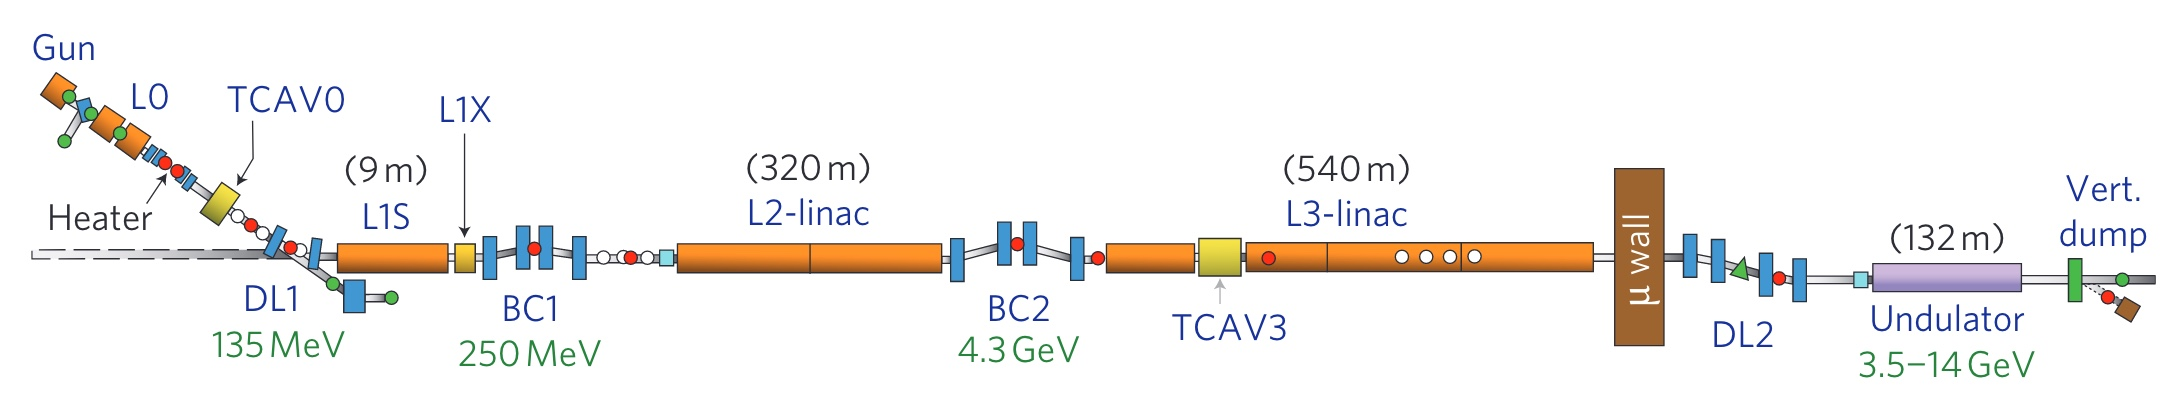
\includegraphics[width=\textwidth]{Figuras/ch1_lcls.png}
  \caption{Esquema del \acrshort{lcls} \autocite{Emma2010}. BC2 y BC2 son dos compresores magnéticos empleados para empaquetar los electrones. Los electrones son acelerados hasta alcanzar \qty{50}{GeV} utilizando radiofrecuencias de \qty{2,856}{MHz}.}
  \label{fig:1.18}
\end{figure}

\paragraph{Armónicos de alto orden}
La tercera fuente de luz \acrshort{xuv} coherente, y protagonista de este trabajo, es la conocida como generación de armónicos de alto orden o \emph{\acrfull{hhg}}. Estos armónicos de alto orden o \emph{\acrfull{hoh}} son producto de la interacción de un láser muy intenso con átomos de un blanco (normalmente gaseoso, aunque también puede ser sólido), provocando la emisión de pulsos ultracortos (femtosegundos y attosegundos) de frecuencias puras impares ($3 \omega, 5 \omega, \ldots$) del haz láser incidente. 

El proceso de formación de los pulsos sigue tres etapas \autocite{Corkum2007}, esquematizadas en la Figura \ref{fig:1.19}. Primero, un campo láser cercano al infrarrojo ---llamado \emph{\acrfull{nir}}--- muy intenso y polarizado linealmente proporciona a los electrones suficiente energía para, por efecto túnel, atravesar la barrera de potencial que lo mantiene ligado al núcleo del átomo, produciéndose su ionización. La probabilidad de la ionización depende del tiempo transcurrido en un periodo de onda del haz \acrshort{nir}. Para $\lambda = \qty{800}{nm}$ (periodo de oscilación de $T_{osc}=\qty{2.7}{fs}$), el tunelamiento es más probable en torno a \qty{300}{as} alrededor del máximo de intensidad (un pico) del campo.

En segundo lugar, el electrón en su movimiento sigue trayectorias con energías cinéticas de \qtyrange{5}{1000}{eV}, proporcionadas por el campo láser durante el primer femtosegundo después de la ionización. Las trayectorias recorridas por los electrones después de la ionización termina en un reencuentro o colisión con el ión, de manera que las trayectorias con mayor energía cinética (las más importantes) están poblados por electrones liberados $\sim T_{osc}/20$ tras una cresta del campo, chocando con el ión $2T_{osc}/3$ después con la energía cinética máxima. 

Finalmente, el electrón es dispersado inelásticamente por el núcleo cuando regresa hacia el ión. Esta colisión tiene una probabilidad de emitir fotones en un pulso de attosegundos de duración. Desde una perspectiva cuántica, la ionización divide el estado del átomo en dos funciones de onda, $\Psi_{G}$ para el ión, y $\Psi_{C}$ para el electrón \autocite{Krausz2009}. Cuando la función de onda del electrón regresa, por acción del campo láser, hasta el estado base $\Psi_{G}$, el patrón de interferencia transfiere la energía cinética, fase y amplitud del electrón dispersado al fotón emitido. De esta forma, controlando la forma y amplitud del pulso láser original puede obtenerse un pulso de armónicos con energía, fase y amplitud específicas.

Los armónicos de alto orden conservan la polarización del haz incidente, así como propiedades ópticas de coherencia y duración del pulso, convirtiéndose en fuentes de radiación \acrshort{xuv} óptimas para su utilización en multitud de aplicaciones, como la observación de la dinámica de los electrones ligados a los núcleos atómicos \autocite{Hentschel2001}, espectroscopía molecular \autocite{Li2008}, y la formación de imágenes \autocite{Ravasio2009}.

Históricamente \autocite{Popmintchev2010}, la observación de los armónicos de alto orden (y, en cierta forma,el surgimiento de la óptica no lineal) la realizó Peter Franken \emph{et al}, en 1961 \autocite{Franken1961}, focalizando la luz de un láser de rubí (muy parecido al utilizado por Maiman \autocite{Maiman1960}) en un cristal de cuarzo, y observando que una pequeña porción de la luz láser emitida era transformada en el segundo armónico. En cualquier caso, el verdadero potencial de la óptica no lineal fue descubierto \autocite{Bloembergen1982} cuando se comprendió como los armónicos generados en el seno de una fuerte polarización son amplificados al propagarse a través del medio óptico no lineal.

En este contexto, el físico Nicolaas Bloembergen y sus colaboradores \autocite{Armstrong1962} desarrollaron las técnicas que permitían convertir de forma eficiente la longitud de onda de la luz láser en otra distinta. Por aquel entonces, a principios de la década de 1960, la transformación de longitudes onda cortas estaba enmarcada en el régimen perturbativo de la óptica no lineal. En este régimen, el medio óptico no sufre daños provenientes de la interacción no lineal con la luz, que es una consecuencia de perturbaciones de bajo orden, mientras que las perturbaciones de alto orden pierden importancia en el proceso. Como consecuencia, la generación de luz ultravioleta con $\lambda \sim \qty{100}{nm}$ (clasificada como \emph{\acrfull{vuv}}) requería utilizar láseres de excímeros o la generación de armónicos convencionales para producir ultravioletas cercanos ($\lambda \sim$ \qtyrange{300}{400}{nm}), seguido por la utilización de resonancias atómicas utilizando las técnicas de Bloembergen \autocite{Popmintchev2010}.

\begin{figure}[htbp]
  \centering
  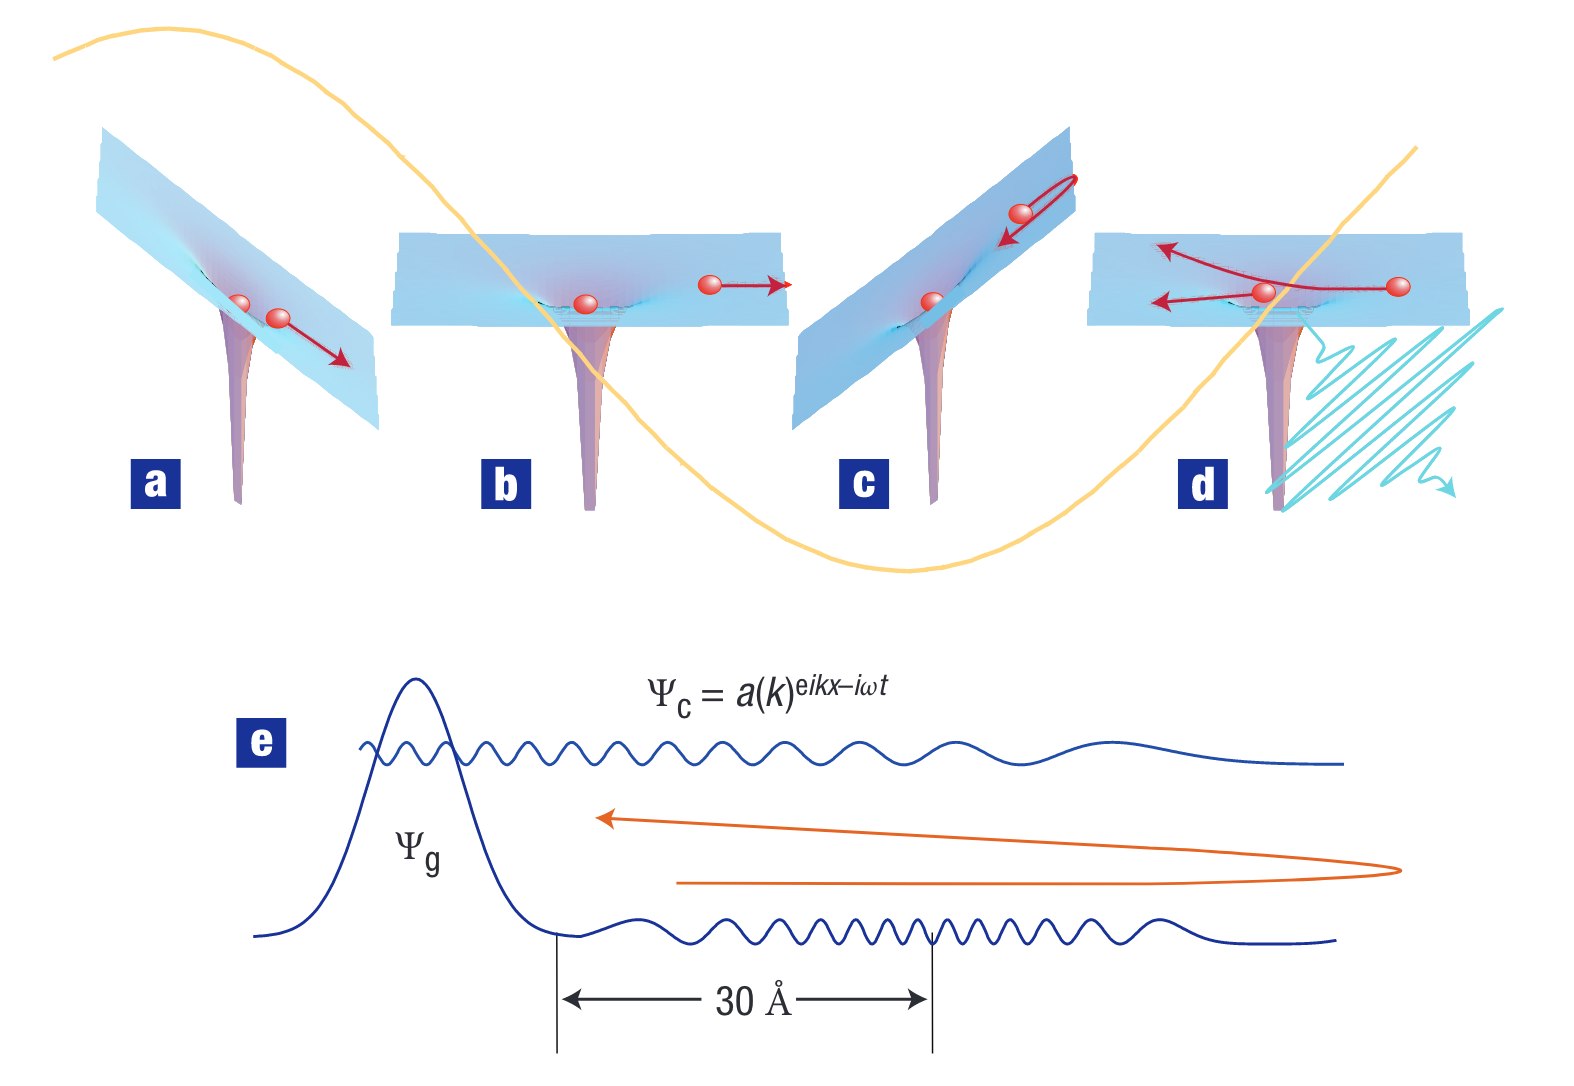
\includegraphics[width=0.7\textwidth]{Figuras/ch1_hhg.png}
  \caption{\textbf{a-d}, Etapas seguidas en la creación de un armónico de alto orden. \textbf{e}, Interferencia de las funciones de onda del ión y el electrón. \autocite{Corkum2007}.}
  \label{fig:1.19}
\end{figure}

Este problema desapareció en 1987, cuando Mcpherson \emph{et al} descubrieron accidentalmente la generación de armónicos de alto orden (\acrshort{hhg}) \autocite{McPherson1987}, mientras realizaban unos experimentos para estudiar la formación de armónicos de bajo orden en régimen perturbativo. En estos experimentos, observaron un número elevado de armónicos impares del haz láser incidente (un láser de \ce{KrF^*} a \qty{248}{nm}), correspondientes a la combinación coherente de un número impar de fotones ($3 \omega, 5 \omega, 7 \omega, 9 \omega, 11 \omega, 13 \omega, 15 \omega$ y $17 \omega$). Además, la intensidad de los armónicos no disminuía significativamente, como predecían los métodos perturbativos. Las observaciones volvieron a repetirse al poco tiempo utilizando láseres infrarrojos \autocite{Ferray1988} (como ocurre en casi todos los experimentos actuales) que reproducían nuevas combinaciones de frecuencias puras (hasta el armónico $31 \omega$).

La formación exclusivamente de armónicos de orden impar puede explicarse por la simetría ante inversión espacial de un medio gaseoso, provocando la eliminación de los armónicos de frecuencias pares \autocite{Milonni1988}. Sin embargo, era necesario desarrollar un formalismo más allá de la óptica no lineal perturbativa para entender por qué estos medios no lineal podían producir múltiples armónicos simultáneamente de intensidades comparables. La clave para entender los fenómenos microscópicos subyacentes del \acrshort{hhg} está en comprender la respuesta de los átomos a campos láser muy intensos.

A principios de 1980, este área estaba siendo estudiada, tras haber sido observadas y estudiadas las múltiples ionizaciones por encima del umbral en átomos de xenón producidas mediante un láser \ce{Nd{:}cristal} (con $\hslash \omega = \qty{1.17}{eV}$) \autocite{Agostini1979}. En 1988, Kulander \emph{et al} \autocite{Kulander1989} simularon la ecuación de Schrödinger dependiente del tiempo para estudiar la ionización del átomo a causa de un campo láser intenso, reproduciendo satisfactoriamente el espectro de los múltiples armónicos producidos del \acrshort{hhg} en el experimento de Ferray \emph{et al}\autocite{Ferray1988}. Otros trabajos habían discutido el proceso de \acrshort{hhg} incluso antes, en 1982 \autocite{Shore1987,Gontier1982}, suponiendo que se trataba de una forma de dispersión de Raman entre estados continuos, y describiendo la etapa de colisión en términos clásicos en el contexto de la ionización múltiple observada \autocite{Kuchiev1987}.

Pocos años después, terminó de establecerse formalmente la descripción del modelo de tres etapas ---explicado anteriormente--- para el proceso de \acrshort{hhg}, esto es, liberación del electrón del átomo sometido al campo láser intenso; aceleración del electrón mediante cesión de energía del campo láser; y recombinación con el ión, emitiendo el exceso de energía cinética como un fotón de alta energía. La relación explícita entre la energía del fotón emitido por \acrshort{hhg} y el potencial ponderomotriz del electrón sometido al campo láser puede emplearse para conocer la energía máxima del fotón \acrshort{hhg}, tal que
\begin{align}
  \label{eq:1.64a}
  E_{\mathrm{cut-off}} &\approx I_{p} + 3,17U_{p} \approx I_{L} \lambda^{2}_{L}, \\
  \label{eq:1.64b}
  U_{p} &= \frac{e^{2}E^{2}_{L}}{4m_{e} \omega^{2}},
\end{align}
donde $I_{p}$ es el potencial de ionización del átomo y $U_{p}$ es la energía ponderomotriz del electrón en un campo muy intenso (la energía media del electrón bajo el campo eléctrico oscilante de un láser con intensidad $I_{L}$ y longitud de onda $\lambda_{L}$). La ecuación \eqref{eq:1.64a} fue identificada por primera vez mediante simulaciones cuánticas \autocite{Krause1992,Kulander1993}, y también puede obtener a partir de la segunda ley de Newton ($F = m_{e}a = -eE_{L}$) aplicada a un electrón libre de carga $e$, masa $m_{e}$, y aceleración $a$ en un campo eléctrico de amplitud $E_{L}$ \autocite{Corkum1993}.

Estos modelos, que fueron desarrollados \emph{a posteriori} para ajustarse a las observaciones llevadas a cabo hasta el momento, terminaron de \enquote{pulirse} poco después con pruebas más rigurosas y sistemáticas \autocite{Chang1997}. El crecimiento lineal del \emph{cut-off} de los armónicos con la intensidad láser (cuya posición, de acuerdo con la ecuación \eqref{eq:1.64a}, es $q_{\mathrm{max}} \approx (I_{p}+3,17U_{p})/\hslash \omega$) significa que los armónicos pueden generarse con energías de los fotones muy elevadas, simplemente aumentando la intensidad o la longitud de onda del láser incidente \autocite{Spielmann1997}, siguiendo la gráfica de la Figura \ref{fig:1.20}.

En 1994, el desarrollo de una teoría semiclásica de \acrshort{hhg} mediante campos láser de bajas frecuencias, fue capaz de explicar por qué el espectro de los armónicos de alto orden (de ahora en adelante, denotados por \acrshort{hoh}) decrecía rápidamente para una energía aproximadamente igual a la mostrado en la ecuación \eqref{eq:1.64a}. La teoría utiliza la formulación de la integral de caminos de la ecuación de Schrödinger dependiente del tiempo para resolver el movimiento del electrón, obteniendo una expresión del momento dipolar eléctrico asociado a la trayectoria del electrón, incluyendo las etapas de ionización, propagación y recombinación, pero manteniendo la naturaleza cuántica ondulatoria del electrón libre sometido al campo láser, siendo
\begin{equation}\label{eq:1.65}
x(t) = \iu \int_{0}^{t} \symrm{d}t\prime \int \symrm{d}^{3}\bar{p}\,\symrm{d}^{*}_{x}[\bar{p}-\bar{A}_{L}(t)]\eu^{-\iu S(\bar{p},\,t,\,t \prime)} E_{L}(t \prime )\symrm{d}_{x}[\bar{p}-\bar{A}_{L}(t \prime )] + \mathrm{c.c.},
\end{equation}
con $x(t)$ el desplazamiento del electrón liberado, $p$ la cantidad de movimiento, $A_{L}$ el potencial vector del campo láser, $E_{L}$ el campo eléctrico del láser, $\symrm{d}_{x}$ la componente de la matriz dipolar paralela al eje de polarización, y $\mathrm{c.c.}$ el complejo conjugado de la expresión.

\begin{figure}[htbp]
  \centering
  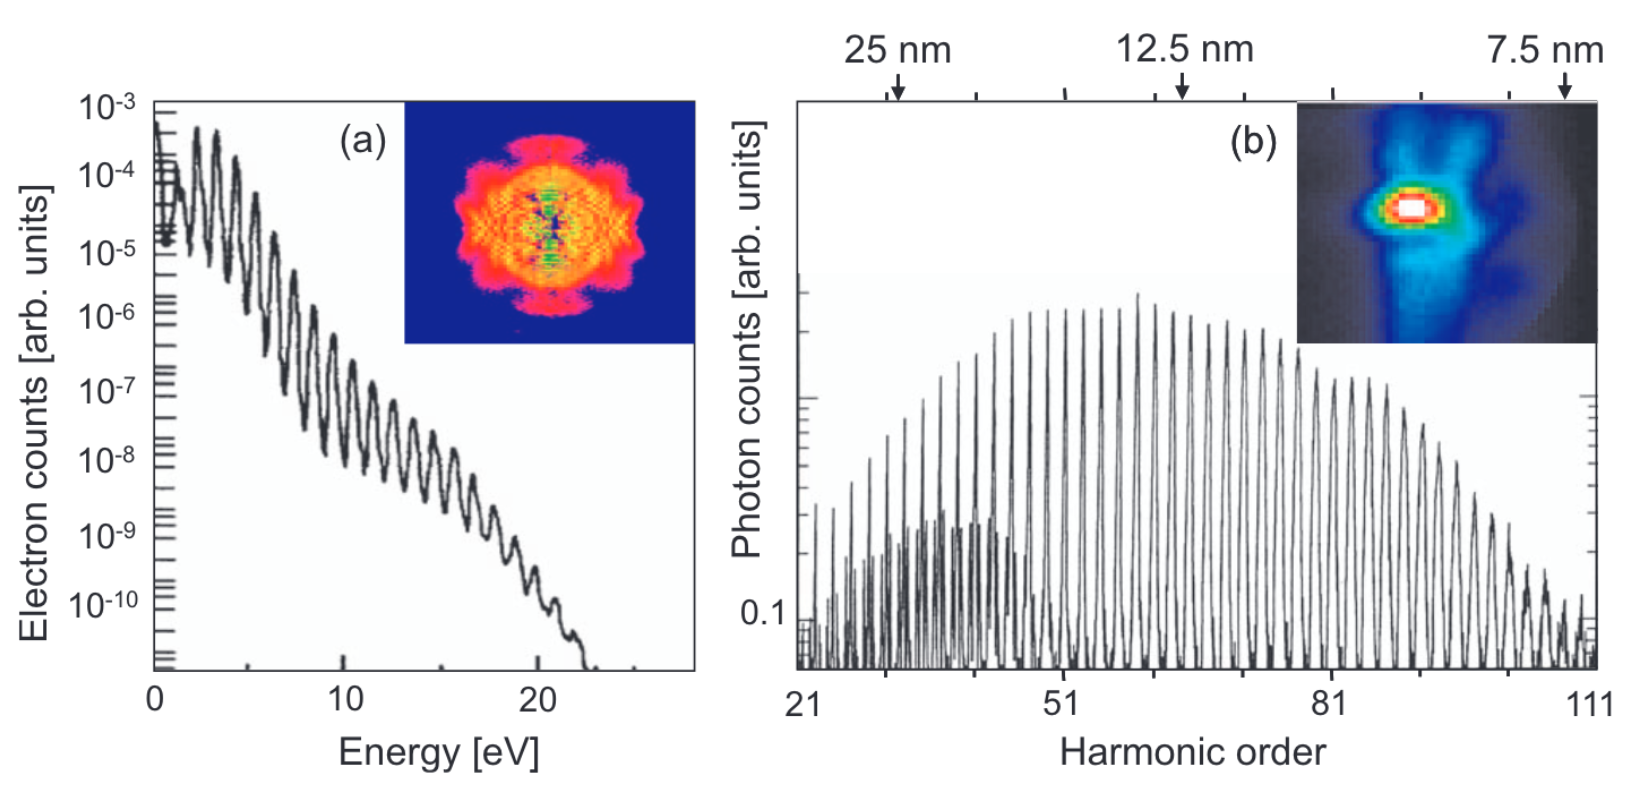
\includegraphics[width=0.6\textwidth]{Figuras/ch1_hhspectra.png}
  \caption{\textbf{a}, Distribución de energía de los electrones producidos por ionización multifotón de un pulso láser de femtosegundos. \textbf{b}, Distribución espectral de la emisión de armónicos de alto orden, en función del número de fotones (intensidad) del haz. \autocite{Krausz2009}.}
  \label{fig:1.20}
\end{figure}

En la ecuación \eqref{eq:1.65}, el primer término corresponde con la ionización del átomo, es decir, la transición de un estado ligado a un estado libre. El segundo término, $\eu^{-\iu S(\bar{p},\,t,\,t \prime )}$, siendo $S$ la integral de acción, describe como la fase de la función de onda del electrón evoluciona durante el $\sim \qty{1}{fs}$ en el que permanece libre antes de la recombinación. El último termino representa el regreso del estado libre al estado ligado. En resumen, el origen de los \acrshortpl{hoh} es consecuencia de la rápida variación espacial y temporal de la función de onda del electrón, que evoluciona cuando un átomo es ionizado por un campo láser intenso. A su vez, esto conduce a la formación de armónicos de muy alto orden a modo de radiación dipolar, incluso cuando se utilizan campos láser con longitudes de onda en el visible.

Además, la ecuación \eqref{eq:1.65} para $x(t)$ puede traducirse con facilidad en una polarización del medio con densidad atómica $n$, tal que $P(t)=-nex(t)$, y a su vez sustituirla en la ecuación de ondas de Maxwell para el campo eléctrico \autocite{Bloembergen1962} (de forma similar a la sección \S\ref{sec:1.2.2}). Sin embargo, el proceso no lineal de \acrshort{hhg} no es instantáneo, como señalaba el segundo término de la ecuación \eqref{eq:1.65}, pues existe un desfase entre el campo láser inicial y la respuesta dipolar del medio responsable de la emisión de los armónicos. El desfase puede ser considerablemente grande ($\gg \pi$), porque el electrón libre puede oscilar recorriendo trayectorias largas con longitudes de onda cortas. 

Este último hecho implica la necesidad de utilizar técnicas avanzadas, conocidas como \emph{\acrfull{qpm}}, para hacer coincidir (idealmente) la velocidad de fase del campo láser incidente y los armónicos, de forma que la emisión armónica de muchos átomos del gas contribuya a una suma coherente de los mismos, permitiendo una conversión de frecuencias eficiente durante la fuerte polarización no lineal del medio. Introducir con éxito estas técnicas fue un reto tecnológico y científico increíble, y aunque no continuará apareciendo en esta discusión, conseguir desarrollar estos métodos ha permitido alcanzar propiedades ópticas en los pulsos láser \acrshort{xuv} inimaginables.

Por último, mencionar la particular idea de introducir un \acrshort{oam} durante el proceso de \acrshort{hhg}. Los haces láser que incorporan \acrshort{oam} con longitudes de onda altas pueden emplearse como semilla para obtener \acrshortpl{hoh} de alta frecuencia, conservando el \acrshort{oam} del pulso inicial. La adición de \acrshort{oam} a un pulso \acrshort{xuv} ultracorto y coherente, producido a partir de una semilla de armónicos, introduce un nuevo \enquote{grado de libertad} en las propiedades de la luz láser que, probablemente descubrirá nuevas aplicaciones. La Figura \ref{fig:1.21} representa gráficamente este concepto, representando un chorro de gas argón como medio óptico no lineal.

Hace 10 años, Hernández-García \emph{et al} (2013) \autocite{Hernandez-Garcia2013} realizaron unas simulaciones de la propagación de un pulso infrarrojo intenso con \acrshort{oam} a través de un gas de argón, y observaron que los armónicos producidos no solamente conservaban los vórtices ópticos propios del \acrshort{oam}, sino que la carga topológica $l \prime $ resultante era $l \prime =q l$, con $q$ el orden del armónico y $l$ la carga topológica del láser infrarrojo. La confirmación experimental la realizaron Gariepy \emph{et al} \autocite{Gariepy2014} al año siguiente, en 2014, utilizando como parámetro $l=1$ para el pulso inicial infrarrojo (con $\lambda = \qty{800}{nm}$), confirmando que los armónicos de orden $n$ generados poseían un \acrshort{oam} con $l \prime = n$, y por tanto el \acrshort{oam} incidente \enquote{sobrevivía} la interacción a través del gas de argón.

Aunque, como ya se ha mencionado, el objetivo de este proyecto no consiste principalmente en estudiar este tipos de haces, las últimas simulaciones, que estudiará el capítulo \ref{cap:4}, introducen \acrshort{oam} sobre el pulso analizado. Adelantando los parámetros empleados, el código utilizado para las simulaciones numéricas introducirá sobre el armónico estudiado (el número $25$ de un pulso infrarrojo con $\lambda = \qty{800}{nm}$) una carga topológica $l=25$ y un índice radial $p=0$, siendo entonces la carga topológica del campo infrarrojo $l=1$.

\begin{figure}[htbp]
  \centering
  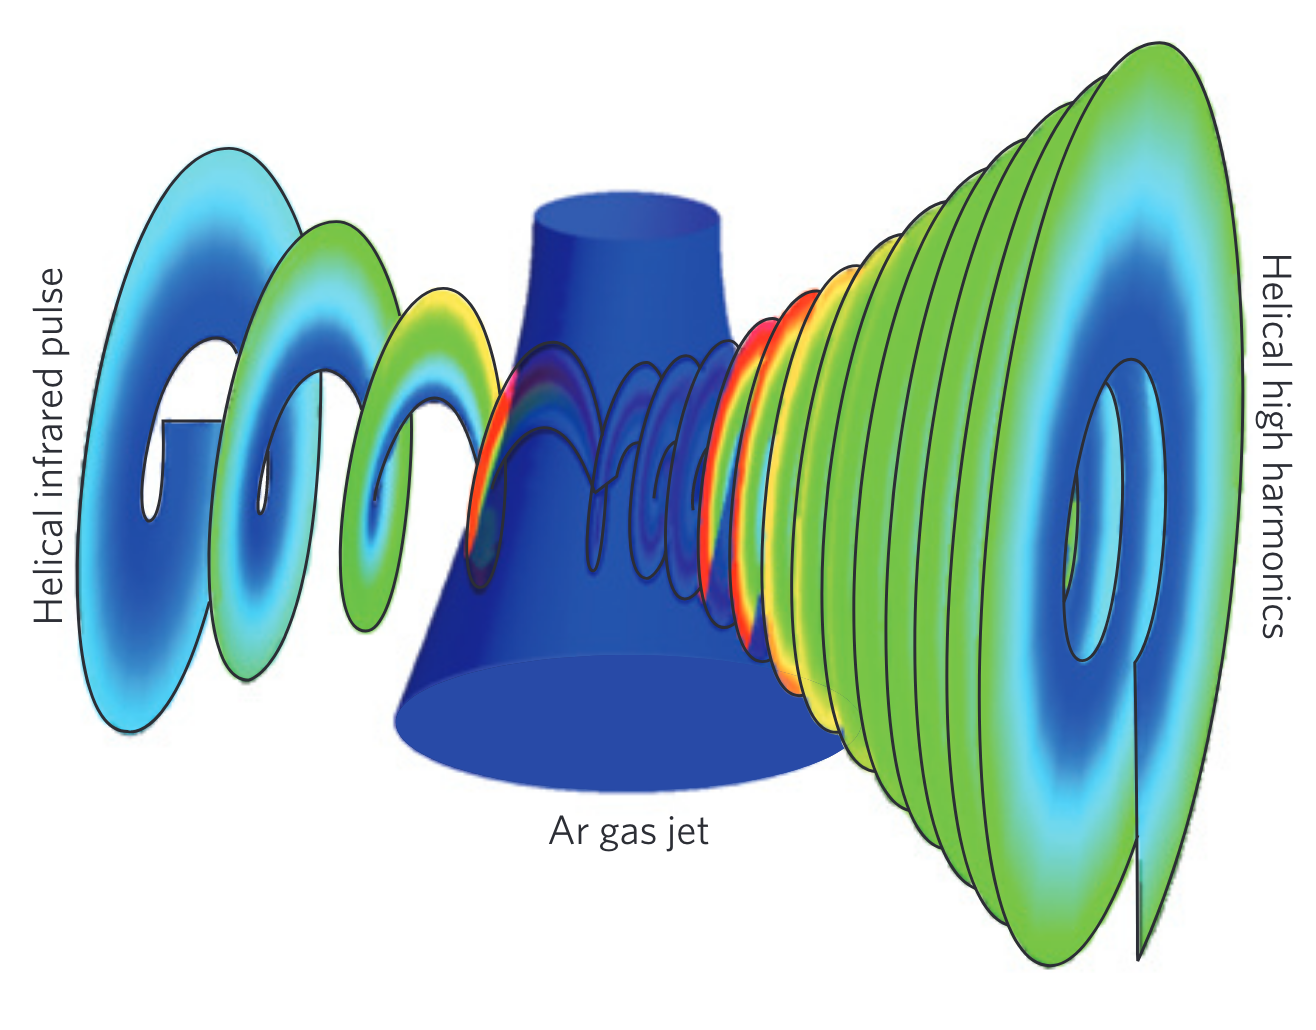
\includegraphics[width=0.5\textwidth]{Figuras/ch1_twist.png}
  \caption{Conversión de un haz láser infrarrojo con \acrshort{oam} al penetrar a través de un medio óptico no lineal en un pulso \acrshort{xuv} ultracorto con \acrshort{oam} \autocite{Patchkovskii2012}.}
  \label{fig:1.21}
\end{figure}

\begin{footheorem*}{Generación de armónicos de alto orden}
  En resumen, la producción de armónicos de alto orden (\acrshort{hhg}) utiliza pulsos infrarrojos intensos sobre blancos gaseosos para obtener pulsos \acrshort{xuv} ultracortos con propiedades ópticas excelentes. El modelo habitual de \acrshort{hhg} sigue tres etapas: 
    \begin{enumerate}
      \item Ionización del átomo gaseoso mediante un pulso láser infrarrojo intenso.
      \item Aceleración del electrón liberado por el campo infrarrojo intenso.
      \item Recolisión del electrón con el ión, liberando el exceso de energía en forma de un pulso ultracorto de armónicos de alto orden.
    \end{enumerate}
\end{footheorem*}
 
\paragraph{Radiación betatrón}
La radiación betatrón como fuente de luz \acrshort{xuv} coherente es, probablemente, la más incipiente y, por tanto, menos desarrollada y estudiada de las formas de producción de rayos X coherentes que existe \autocite{Corde2013}. La proposición y demostración de esta fuente de rayos X tiene su origen en un mecanismo simulado numéricamente por Tajima y Dawson \autocite{Tajima1979}, en 1979, para acelerar electrones hasta velocidades relativistas.

Acelerar electrones hasta velocidades cercanas a la luz es un proceso complejo y costoso, pues requiere emplear aceleradores de partículas de grandes tamaños (basta observar el tamaño de las instalaciones del \acrshort{lcls}, en Livermore, California, o del \acrfull{esrf}, en Grenoble, Francia). Sin embargo, una forma de reducir el tamaño y coste de los futuros aceleradores utilizados en investigación y en desarrollos tecnológicos, consiste en emplear los campos eléctricos extremadamente intensos ($\sim \qty{100}{GV/m}$, mil veces mayores que un sincrotrón convencional) generados en plasmas producidos por láseres para acelerar electrones. Este concepto de aceleradores es conocido como \emph{\acrfullpl{lwfa}} (un acelerador sincrotrón con un tamaño de milímetros).

El método consiste en utilizar un haz láser ultraintenso sobre un blanco sólido o gaseoso, originando un plasma de iones y electrones. Por ejemplo, un pulso láser puede enfocarse sobre chorro de gas, de manera que cuando el frente del pulso se encuentra con la nube de gas, \enquote{arranca} los electrones de las moléculas del gas, formando el plasma de electrones e iones buscado. Este pulso continúa formando una \enquote{nube} de plasma al penetrar a través de la nube gaseosa. La presión de radiación del pulso láser \enquote{empuja} a los electrones de la nube de plasma lejos del frente del pulso láser, similar a como la proa de una barco aleja el agua circundante en su desplazamiento. Los iones, que son mucho más pesados que los electrones, no pueden ser desplazados por el pulso láser, formándose una \enquote{burbuja} de iones cargados positivamente a su paso.

De la misma forma que parte del agua empujada por la proa de un barco lo rodea y termina atrapada por la estela formada por el movimiento de la embarcación, los electrones echados a un lado por el pulso dan la vuelta y son atrapados por la estela del pulso, es decir, la burbuja de iones. Los electrones que siguen la estela experimentan una fuerte aceleración a través de la burbuja de iones, oscilando rápidamente siguiendo una trayectoria senoidal y emitiendo rayos X, como muestra la Figura \ref{fig:1.22}.

Entre las primeras observaciones experimentales del haz de electrones, a finales de la década de $1990$, \autocite{Modena1995,Umstadter1996} se utilizaron pulsos láser de $\sim \qty{1}{ps}$, y desde entonces las energías del haz de electrones han aumentado hasta \qtyrange{60}{170}{MeV} \autocite{Mangles2004,Faure2004,Geddes2004} empleando pulsos láser ultracortos de $\sim \qty{100}{fs}$. Por otro lado, la proposición y demostración de la emisión de rayos X en \acrshortpl{lwfa} tuvo lugar en $2004$ \autocite{Kostyukov2004,Rousse2004}, convirtiéndose en la primera fuente de luz \acrshort{xuv} coherente y colimada originada directamente mediante una interacción láser-plasma. Los años sucesivos estuvieron marcados por la caracterización y medición de la radiación betatrón en regímenes de interacción desde los teravatios \autocite{TaPhuoc2005,TaPhuoc2007,TaPhuoc2012,Shah2006,Albert2008} hasta los petavatios \autocite{Kneip2008,Kneip2010} de potencia. 

La amplia diversidad y dificultad de esta fuente queda patente en la multitud de artículos y publicaciones científicas que protagonizan. En física fundamental, la utilización de \acrshortpl{lwfa} permite estudiar y validar experimentalmente predicciones en electrodinámica cuántica \autocite{Cole2018,Poder2018}, accediendo a intensidades y energías de interacción inalcanzables anteriormente; y en física de aceleradores, los \acrshortpl{lwfa} han demostrado ser útiles para sustituir a los grandes aceleradores en la exploración de los haces de partículas monoenergéticos de alta energía \autocite{Gotzfried2020,Gilljohann2019} 

Desde el prisma de la tecnología y sus posibles aplicaciones, Kozlova \emph{et al} \autocite{Kozlova2020} han introducido gradientes de densidad en el plasma y realizado simulaciones que demuestran una mejora del flujo y energía de la radiación betatrón, sin aumentar la energía del pulso láser; Maier \emph{et al} \autocite{Maier2020} han conseguido incrementar el número de electrones del haz acelerado (paquetes de $100000$ electrones en $24$ horas), que supone un avance importante en metrología; y Debus \emph{et al} \autocite{Debus2019} han propuesto un esquema con dos láseres pulsados que permite superar el umbral de energía alcanzada por los electrones y los rayos X emitidos. 

\begin{figure}[htbp]
  \centering
  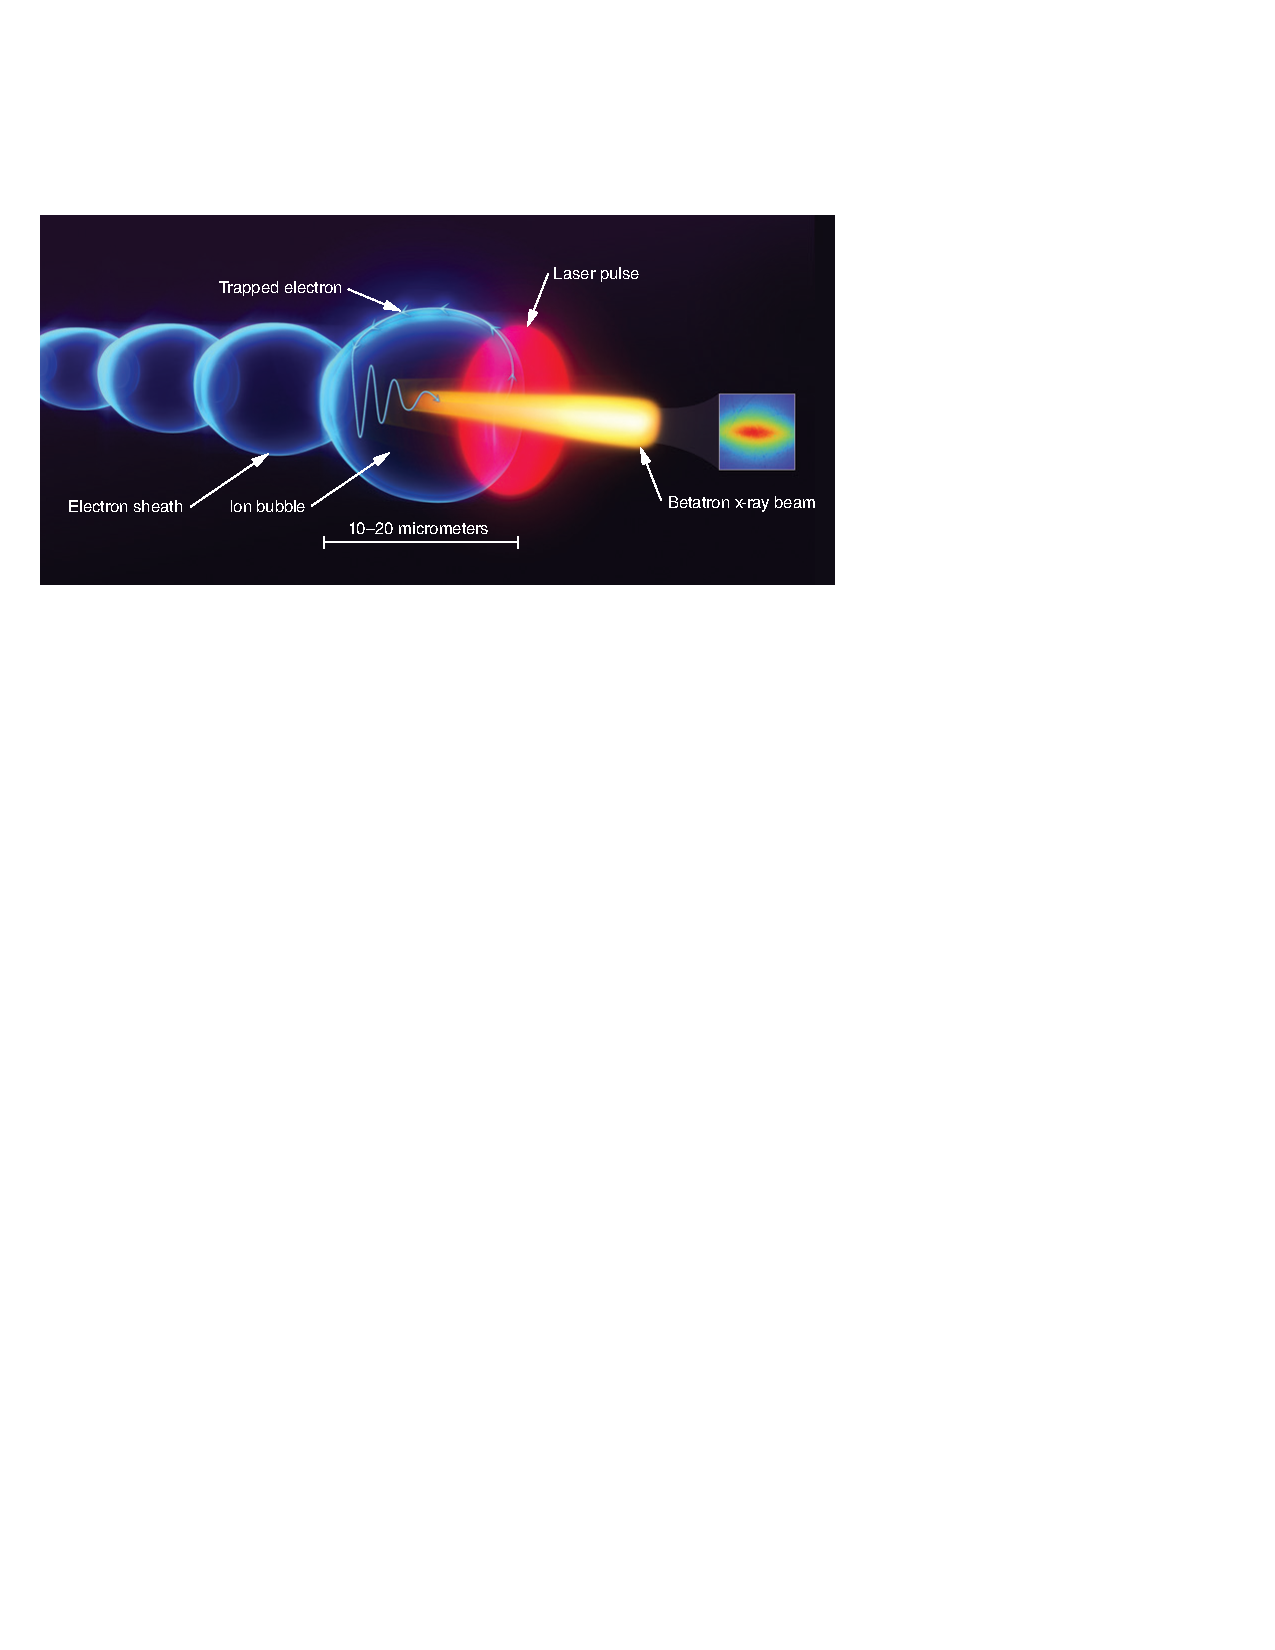
\includegraphics[width=0.69\textwidth]{Figuras/ch1_betaxrays.pdf}
  \caption{Representación de la emisión de radiación X betatrón y del haz de electrones en un \acrshort{lwfa}. Parker, A. (enero de 2014). \emph{Betatron X-rays Bring Focus to a Very Small, Very Fast World}. Lawrence Livermore National Laboratory. \url{https://str.llnl.gov/january-2014/albert}.}
  \label{fig:1.22}
\end{figure}

\section{Láseres de rayos X basados en plasmas}\label{sec:1.4}
Después de presentar los distintos tipos de fuentes de radiación \acrshort{xuv} coherente, una pregunta que todavía no ha sido respondida es: ¿qué son exactamente?, y ¿qué posición ocupan en el espectro electromagnético? Pues bien, la radiación ultravioleta extrema (\acrshort{xuv}) o rayos X blandos son denominaciones intercambiables que hacen referencia a radiaciones con energías comprendidas entre los \qty{20}{eV} y \qty{600}{eV}, aunque este intervalo es, en general, variable. 

De esta manera, los láseres de rayos X basados en plasmas o \emph{\acrfullpl{sxrl}}, protagonistas indiscutibles en este proyecto, son aquellos que emplean un plasma como medio activo para conseguir luz láser en el rango de los ultravioletas extremos (\acrshort{xuv}) o rayos X blandos. Obtener un efecto láser de estas energías en la materia fue complicado por diversos motivos. Entre estos se encuentran, recordando la ecuación \eqref{eq:1.8b}, el dominio natural de la emisión espontánea frente a la emisión amplificada a altas frecuencias, y las elevadas energías necesarias para bombear los niveles energéticos de los átomos que participan en la emisión de rayos X blandos. 

La primera propuesta \autocite{Duguay1967} relacionada con este último aspecto, estaba basada en la fotoionización de átomos de boro y zinc, y apareció en $1967$. Sin embargo, la propuesta fracasó porque los átomos implicados necesitaban fuentes de bombeo que depositaran energía en los rayos X para conseguir la inversión de población (era un círculo vicioso), y en la década de $1960$ no disponían de la tecnología necesaria. Algunas ideas, más extravagantes y absurdas \autocite{Thorne2017} (que afortunadamente tampoco funcionaron), surgieron en Estados Unidos durante la presidencia de Ronald Reagan, y tenían como objetivo desarrollar un \enquote{super láser de rayos X} bombeado mediante la detonación de una bomba nuclear para derribar misiles soviéticos.

Otra pregunta que cabría hacerse es ¿por qué es necesario un plasma como medio activo? La respuesta es breve, las transiciones electrónicas disponibles capaces de emitir luz \acrshort{xuv} de forma \enquote{sencilla} están presentes en ciertos átomos fuertemente ionizados, en decir, ¡en un plasma de iones y electrones! La explicación precisa requiere de la teoría cuántica \autocite{Sakurai2020}. Cuando un átomo sufre múltiples ionizaciones, la \enquote{distancia} entre niveles de energía (la línea de emisión) aumenta progresivamente con el grado de ionización, reduciéndose la longitud de onda asociada a la transición entre niveles energéticos, y aumentando por tanto la energía de los fotones liberados durante la emisión. 

Escogiendo un átomo de un elemento químico determinado, por ejemplo, kriptón o xenón, e ionizándolos hasta conseguir una estructura electrónica idéntica a otro elemento químico (familias de iones isoelectrónicos), por ejemplo, níquel, (iones $\ce{Kr}^{8+}$ y $\ce{Xe}^{16+}$, ambos con $28$ electrones en su capa de valencia, como el níquel) experimentalmente puede observarse un movimiento hacia energías superiores de los niveles electrónicos que participan en las transiciones ópticas o ultravioletas buscadas. 

Regresando a la cuestión del plasma como amplificador, hay que subrayar algunos aspectos claves de su utilización. Las temperaturas necesarias para obtener una emisión \acrshort{xuv} coherente son de \qtyrange{0.1}{1}{keV}, mientras que las densidades que permiten su propagación eficiente a través del plasma oscilan los \qtyrange{e18}{e21}{cm^{-3}}. Además, producir la inversión de población y aprovecharla correctamente resulta muy complejo técnicamente, como se mencionó anteriormente, especialmente cuando las frecuencias buscadas son elevadas. 

Actualmente existen dos conceptos básicos para reproducir en un laboratorio estas características, posteriores a la idea original (fallida) de la fotoionización: la \emph{recombinación} y el \emph{bombeo colisional}. 

\paragraph{Recombinación}
Esta esquema consiste en generar un plasma de alta densidad electrónica con la temperatura necesaria (un grado de ionización determinado) para la emisión. Después, la expansión hidrodinámica del plasma y las pérdidas por radiación enfrían rápidamente los electrones libres del plasma, perdiendo energía y dominando una etapa de recombinación con los iones para ocupar las posiciones más externas de la corteza electrónica. Este proceso dominante es conocido como \emph{recombinación de tres cuerpos}, donde un electrón libre $e$ en las inmediaciones de un ión positivo \ce{A+}, colisiona con otro segundo electrón $e \prime $, perdiendo energía y provocando su \enquote{caída} en el pozo de potencial del ión, de ahí el nombre del esquema.

La inversión de población de los estados inferiores ocurre cuando los electrones en los niveles superiores mencionados experimentan una sucesión de transiciones electrónicas hacia los niveles inferiores, en busca de la estabilidad (recombinación radiativa), o mediante nuevas recombinaciones de tres cuerpos. La propuesta teórica la realizaron Gudzenko y Shelepin (1964), del Instituto Lebedev de Física de Moscú\autocite{Gudzenko1964}, para un plasma denso y ultrafrío de hidrógeno; los primeros indicios experimentales (en iones de \ce{Al^{4+}}) fueron observados por Jaeglé \emph{et al} (1971) \autocite{Jaegle1971}; y la demostración experimental unos años más tarde, por Suckewer \emph{et al} (1985)\autocite{Suckewer1985}, enfocando un láser de \ce{CO2} sobre un blanco sólido de carbono.

\paragraph{Bombeo colisional}
El bombeo colisional, también conocido como \emph{excitación colisional}, es una variación del concepto de bombeo óptico propuesto por Alfred Kastler (1950)\autocite{Kastler1950}, que trabajaba en el Laboratorio de Física de \emph{l’École Normale Supérieure}, en París. Este método, utilizado en este trabajo, recurre a las colisiones entre electrones libres del plasma con los iones para generar una inversión de población. De esta forma, los electrones excitan a los iones, proporcionando la energía necesaria a los electrones ligados de los iones para su promoción hasta la banda de absorción.

Originalmente, fue sugerido teóricamente por Zherikin \emph{et al} (1976) y Vinogradov \emph{et al} (1977), que además, demostraron la posibilidad de conseguir una emisión de luz \acrshort{vuv} en ciertas transiciones de iones neonoides ($10$ electrones). La confirmación experimental de luz \acrshort{xuv} tuvo lugar unos años más tarde, en 1985 \autocite{Matthews1985,Rosen1985}, apoyándose en iones de selenio e itrio neonoides y técnicas espectroscópicas para medir las ganancias obtenidas, con coeficientes de ganancia de \qty{5.5 +-  1.0}{cm^{-1}}.

En general, la utilización de familias de iones heliumoides (2 electrones), neonoides (10 electrones), niqueloides (28 electrones) y paladiumoides (46 electrones) tiene el propósito de conseguir el mayor número de iones estables electrónicamente en el plasma, pues su banda de valencia está completa. Por otra parte, el plasma debe reunir unas condiciones iniciales básicas, a partir de las cuales pueda producirse la emisión \acrshort{xuv}. Esencialmente, como tratará la sección \S\ref{sec:3.3}, la radiación \acrshort{xuv} tiene que propagarse a través del plasma sin \enquote{escaparse} de sus fronteras, planteando la necesidad de una distribución de electrones que mantenga el haz láser dentro del plasma, pero favoreciendo un equilibrio que permita mantener una inversión de población favorable.

Para conseguir un láser \acrshort{xuv} con iones niqueloides (como los iones de $\ce{Kr^{8+}}$ de este proyecto), hubo que esperar a MacGowan \emph{et al} (1987)\autocite{MacGowan1987}, en el \emph{\acrfull{llnl}}. El experimento mostró la amplificación de la emisión espontánea entre \qtyrange{6.583}{7.1}{nm}, después de enfocar un láser ultracorto muy intenso sobre una lámina delgada de \ce{EuF2}, formando iones de europio niqueloide $\symrm{Eu}^{+35}$ responsables de la transición. También sugirieron la posibilidad de extrapolar sus resultados a iones de \ce{Yb^{+43}}, así como cierta evidencia de amplificación en iones de \ce{W^{+46}}.

\begin{figure}[htbp]
  \centering
  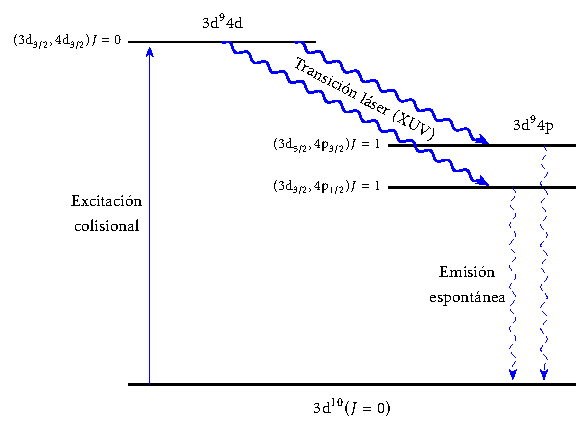
\includegraphics[width=0.7\textwidth]{Figuras/ch1_niquel_like.pdf}
  \caption{Esquema simplificado de los niveles de energía que participan en la transición láser de un ión niqueloide. Adaptado de G. J. Tallents (2003) \autocite{Tallents2003}.}
  \label{fig:1.23}
\end{figure}

El diagrama de energía de los iones niqueloides aparece en la Figura \ref{fig:1.23}. El efecto láser tiene lugar gracias a las transiciones $\symrm{3d^{9}4d \rightarrow 3d^{9}4p}$ entre los dos estados del nivel energético inferior y el estado del nivel superior. El diagrama está simplificado, porque la inversión de población del nivel superior $\symrm{3d^{9}4d}$ tiene una segunda vía formada por la transición $\symrm{3d^{10} \rightarrow \symrm{3d^{9}4f}}$ (también por colisiones con los electrones), seguida por una emisión no radiativa hasta el nivel energético de bombeo $\symrm{3d^{9}4d}$ (el estado ocupado es inestable). En cualquier caso, el nivel inferior es despoblado rápidamente mediante la emisión espontánea de radiación. La sección \S\ref{sec:3.4} mostrará un esquema expandido para el caso del ión \ce{Kr^{8+}}.

Una ventaja de los iones niqueloides frente a los neonoides es que necesitan depositar menos energía durante el bombeo para conseguir la misma amplificación de luz \acrshort{xuv}. A igual número de electrones arrancados de la banda de valencia, los iones niqueloides poseen niveles energéticos con transiciones a longitudes de onda más cortas, y por tanto, de mayor energía en la emisión. Sin embargo, la amplificación de los iones neonoides superaba a los niqueloides, por lo que la pérdida de ganancia no estaba siendo compensada por la menor exigencia energética. A finales de la década de 1990, aparecieron nuevos experimentos y tecnologías capaces de eliminar este inconveniente, llegando incluso a alcanzar el régimen de saturación. 

Por ejemplo, Zhang \emph{et al} (1997)\autocite{Zhang1997} demostraron una emisión láser de rayos X de \qty{0.3}{mJ} ($\lambda = \qty{7}{nm}$) con pulsos de \qty{50}{ps} y ganancias de \qty{8.4 +- 0.6}{cm^{-1}}, enfocando un sistema láser de \ce{Nd{:}cristal} (\qty{1.05}{µm}, \qty{75}{ps}) sobre un doble blanco de samario (el ión niqueloide responsable de la transición) en un soporte de vidrio. El doble blanco permitía aumentar el pico de ganancia y reducir el ángulo de divergencia a la salida de los rayos X ($\Delta \theta \approx \qty{1}{mrad}$), mientras que el sistema láser generaba múltiples pulsos capaces de \enquote{preformar} un plasma inicial, cuya menor densidad electrónica facilitaba la propagación de los rayos X. De esta forma, alcanzar la saturación en rayos X permite extraer la máxima potencia posible para un volumen del plasma determinado, añadiendo una mejor escalabilidad de la longitud de onda del ión niqueloide con las fuentes de bombeo.

Es importante mencionar que todos los progresos mencionados hasta ahora recurrían a un plasma en estado \emph{cuasi-estacionario}, es decir, manteniendo sus propiedades constantes en el tiempo durante el intervalo de estudio ($\sim \qty{100}{ps}$). La excitación colisional que emplea este esquema es conocida por el nombre de \emph{\acrfull{qss}}. Esta técnica \autocite{Rus2002} recurre a un primer pulso infrarrojo intenso ultracorto ($\sim  \qty{100}{J}$, $\sim \qty{1}{ns}$) para, simultáneamente, ionizar un blanco sólido (ablación), formando el plasma amplificador, e incrementar la energía de los electrones encargados de producir la inversión electrónica (calentamiento).

Además, existe un segundo esquema de excitación colisional llamado \emph{\acrfull{tce}} \autocite{Nickles1997}, que utiliza dos pulsos láser distintos para producir el plasma y calentar los electrones. Durante la primera etapa, un pulso infrarrojo ($\sim \qty{100}{ps}$) origina las especies electrónicas que constituyen el plasma. Después, la segunda etapa enfoca otro pulso infrarrojo ultracorto ($\sim \qty{1}{ps}$), depositando su energía en los electrones que excitarán los iones del plasmas. Esta alternativa tiene la ventaja de controlar con mayor precisión la estructura del plasma obtenido, regulando el tiempo de retardo entre ambos pulsos en \acrshort{tce}, mientras que la energía necesaria es inferior a la requerida en el \acrshort{qss}. Naturalmente, el segundo pulso debe calentar los electrones rápidamente, antes de producir nuevas ionizaciones de los iones amplificadores.

Sin embargo, aunque la ganancia máxima aumenta en el \acrshort{tce} su duración disminuye, reduciendo la longitud de aprovechamiento en el medio activo. La solución suele aprovechar el desacoplamiento de los pulsos anteriores para sincronizar la inversión poblacional con la amplificación del pulso \acrshort{xuv} \autocite{Kozlova2020a}. Habitualmente, una fracción importante de los equipos sitúan el láser de bombeo formando un ángulo de inclinación respecto al eje del plasma, solución llamada \emph{\acrfull{grip}} \autocite{Keenan2005}.  

Otra pregunta muy astuta que aparece en estos esquemas, y en las investigaciones presentadas hasta ahora, es: ¿qué luz está siendo amplificada?, ¿qué está provocando la emisión \acrshort{xuv}? La respuesta a ambas preguntas es el \enquote{ruido}. En realidad, los fotones amplificados han sido emitidos espontáneamente desde el nivel superior de la transición láser, ejerciendo como las semillas necesarias para inducir el efecto resonante entre los estados que participan en la emisión \acrshort{xuv}, de ahí la palabra ruido. Por tanto, estos métodos están basados en la amplificación de la emisión espontánea (ruido) de radiación o, en la literatura especializada, \emph{\acrfull{ase}}.

La coherencia temporal obtenida siguiendo estos esquemas es elevada, pero, en cambio, la coherencia espacial sufre una disminución, porque la emisión espontánea (que es aleatoria) es incoherente al producirse en áreas diferenciadas del medio. La propuesta para solventar este contratiempo, como explicará la sección \S\ref{sec:1.4.1}, consiste en inyectar una semilla de \acrshort{hoh} que aproveche sus extraordinarias cualidades ópticas para ser amplificada. En el futuro, también podrían utilizarse sistemas de doble blanco o doble paso por el plasma que proporcionen mejores coherencias espaciales.



\subsection{Inyección de armónicos}\label{sec:1.4.1}

%\subsection{Ionización de efecto campo}\label{sec:1.4.2}




%\section{Estado del arte}\label{sec:1.5}
